\documentclass[11pt]{article}

%%%%%%%%%%%%%%%%%%%%%%%%%%%%%%%%%%%%%%%%%%%
% Commands for customizing the assignment %
%%%%%%%%%%%%%%%%%%%%%%%%%%%%%%%%%%%%%%%%%%%


%% To HIDE SOLUTIONS (to post on the website for students), set this value to 0: \def\issoln{0}
%\providecommand{\issoln}{1}

%-----------------------------------------------------------------------------
% PACKAGES AND OTHER DOCUMENT CONFIGURATIONS
%-----------------------------------------------------------------------------

\usepackage[margin=.75in]{geometry}
\usepackage{amsmath, amsfonts}
\usepackage{enumerate}
\usepackage{graphicx}
\usepackage{titling}
\usepackage{url}
\usepackage{xfrac}
\usepackage{natbib}
\usepackage{amssymb}
\usepackage[export]{adjustbox}
\usepackage{amsthm, mathrsfs}
\usepackage{paralist}
\usepackage{epstopdf}
\usepackage{tabularx}
% \usepackage{longtable}
\usepackage{multirow}
\usepackage{multicol}
\usepackage[colorlinks=true,urlcolor=blue]{hyperref}
\usepackage{algorithm}
\usepackage{algorithmicx}
\usepackage[noend]{algpseudocode}
\usepackage{float}
\usepackage{enumerate}
\usepackage{array}
\usepackage{environ}
% \usepackage{times}
\usepackage{textcomp}
\usepackage{caption}
\usepackage{parskip} % For NIPS style paragraphs.
\usepackage[compact]{titlesec} % Less whitespace around titles
\usepackage[inline]{enumitem} % For inline enumerate* and itemize*
\usepackage{datetime}
\usepackage{comment}
% \usepackage{minted}
\usepackage{color}
\usepackage[table]{xcolor}
\usepackage[final]{listings}
\usepackage{tikz}
\usepackage{framed}
\usepackage{cprotect}
\usepackage{verbatimbox}
\usepackage{multicol}
\usepackage{hyperref}
\usepackage{subcaption}
\usepackage{mathtools} % For drcases
\usepackage{cancel}
\usepackage[many]{tcolorbox}
\usepackage{soul}
\usepackage[bottom]{footmisc}
\usepackage{bm}
\usepackage{wasysym}
\usepackage{setspace}
\setstretch{1.2} 
\usetikzlibrary{tikzmark}
%%%%%%%%%%%%%%%%%%%%%%%%%%%%%%%%%%%%%%%%%%%
% Formatting for \CorrectChoice of "exam" %
%%%%%%%%%%%%%%%%%%%%%%%%%%%%%%%%%%%%%%%%%%%
%%%%%%%%%%%%%%%%%%%%%%%%%%%%%%%%%%%%%%%%%%%
\usepackage{arydshln} % <-- for dashed line on tables
\usepackage{ifthen}
\usepackage{soul}
% \usepackage{fontspec}
% \setmainfont{lmodern} % Latin Modern is the OpenType version of Computer Modern

\usepackage[latin1]{inputenc}
\usepackage[T1]{fontenc}
\usepackage[labelfont=bf]{caption} % Makes all caption labels bold
\captionsetup{font=bf} % Makes all caption text bold

% \usepackage{tgpagella} % best so far 
% \usepackage{tgcursor}[qcr]
\usepackage[euler-digits]{eulervm}
% \usepackage[OT1]{eulervm}

\usepackage[english]{babel}

\newcommand{\mathcolorbox}[2]{\colorbox{#1}{$\displaystyle #2$}}

\usepackage{booktabs, array} % for better spacing and rules

\newboolean{solve}
\setboolean{solve}{true} % Set this to false if you don't want to show the solutions
\tcbuselibrary{skins,breakable}

% enhanced breakable to break the tcolorbox over pages
\newenvironment{solve}{%
  \ifthenelse{\boolean{solve}}{%
    \begin{tcolorbox}[enhanced, breakable, colframe=black, colback=white, coltext = black]
    \noindent \underline{\textbf{Solution:}}
    }{%
  }%
}{ \hfill $\square$
\ifthenelse{\boolean{solve}}{\end{tcolorbox} }{}}
% added \newpage
\newcommand\numberthis{\addtocounter{equation}{1}\tag{\theequation}}
%%%%%%%%%%%%%%%%%%%%%%%%%%%%%%%%%%%%%%%%%%%

% \numberwithin{equation}{section} % Number equations within sections (i.e. 1.1, 1.2, 2.1, 2.2 instead of 1, 2, 3, 4)
% \numberwithin{figure}{section} % Number figures within sections (i.e. 1.1, 1.2, 2.1, 2.2 instead of 1, 2, 3, 4)
% \numberwithin{table}{section} % Number tables within sections (i.e. 1.1, 1.2, 2.1, 2.2 instead of 1, 2, 3, 4)

%%%%%%%%%%%%%%%%%%%%%%%%%%%%%%%%%%%%%%%%%%
% Custom commands                        %



%%%%%%%%%%%%%%%%%%%%%%%%%%%%%%%%%%%%%%%%%%
% Custom commands for Math               %
%%%%%%%%%%%%%%%%%%%%%%%%%%%%%%%%%%%%%%%%%%
\newcommand{\p}{\partial}
\newcommand{\vc}[1]{\boldsymbol{#1}}
\newcommand{\adj}[1]{\frac{\partial \ell}{\partial #1}}
\newcommand{\chain}[2]{\adj{#2} = \adj{#1}\frac{\partial #1}{\partial #2}}
\newcommand{\ntset}{test}
\newcommand{\zerov}{\mathbf{0}}

% mathcal
\newcommand{\Ac}{\mathcal{A}}
\newcommand{\Bc}{\mathcal{B}}
\newcommand{\Cc}{\mathcal{C}}
\newcommand{\Dc}{\mathcal{D}}
\newcommand{\Ec}{\mathcal{E}}
\newcommand{\Fc}{\mathcal{F}}
\newcommand{\Gc}{\mathcal{G}}
\newcommand{\Hc}{\mathcal{H}}
\newcommand{\Ic}{\mathcal{I}}
\newcommand{\Jc}{\mathcal{J}}
\newcommand{\Kc}{\mathcal{K}}
\newcommand{\Lc}{\mathcal{L}}
\newcommand{\Mc}{\mathcal{M}}
\newcommand{\Nc}{\mathcal{N}}
\newcommand{\Oc}{\mathcal{O}}
\newcommand{\Pc}{\mathcal{P}}
\newcommand{\Qc}{\mathcal{Q}}
\newcommand{\Rc}{\mathcal{R}}
\newcommand{\Sc}{\mathcal{S}}
\newcommand{\Tc}{\mathcal{T}}
\newcommand{\Uc}{\mathcal{U}}
\newcommand{\Vc}{\mathcal{V}}
\newcommand{\Wc}{\mathcal{W}}
\newcommand{\Xc}{\mathcal{X}}
\newcommand{\Yc}{\mathcal{Y}}
\newcommand{\Zc}{\mathcal{Z}}
\newcommand{\Lf}{\mathscr{L} }
% mathbb
\newcommand{\Ab}{\mathbb{A}}
\newcommand{\Bb}{\mathbb{B}}
\newcommand{\Cb}{\mathbb{C}}
\newcommand{\Db}{\mathbb{D}}
\newcommand{\Eb}{\mathbb{E}}
\newcommand{\Fb}{\mathbb{F}}
\newcommand{\Gb}{\mathbb{G}}
\newcommand{\Hb}{\mathbb{H}}
\newcommand{\Ib}{\mathbb{I}}
\newcommand{\Jb}{\mathbb{J}}
\newcommand{\Kb}{\mathbb{K}}
\newcommand{\Lb}{\mathbb{L}}
\newcommand{\Mb}{\mathbb{M}}
\newcommand{\Nb}{\mathbb{N}}
\newcommand{\Ob}{\mathbb{O}}
\newcommand{\Pb}{\mathbb{P}}
\newcommand{\Qb}{\mathbb{Q}}
\newcommand{\Rb}{\mathbb{R}}
\newcommand{\Sb}{\mathbb{S}}
\newcommand{\Tb}{\mathbb{T}}
\newcommand{\Ub}{\mathbb{U}}
\newcommand{\Vb}{\mathbb{V}}
\newcommand{\Wb}{\mathbb{W}}
\newcommand{\Xb}{\mathbb{X}}
\newcommand{\Yb}{\mathbb{Y}}
\newcommand{\Zb}{\mathbb{Z}}

% mathbf lowercase
\newcommand{\av}{\mathbf{a}}
\newcommand{\bv}{\mathbf{b}}
\newcommand{\cv}{\mathbf{c}}
\newcommand{\dv}{\mathbf{d}}
\newcommand{\ev}{\mathbf{e}}
\newcommand{\fv}{\mathbf{f}}
\newcommand{\gv}{\mathbf{g}}
\newcommand{\hv}{\mathbf{h}}
\newcommand{\iv}{\mathbf{i}}
\newcommand{\jv}{\mathbf{j}}
\newcommand{\kv}{\mathbf{k}}
\newcommand{\lv}{\mathbf{l}}
\newcommand{\mv}{\mathbf{m}}
\newcommand{\nv}{\mathbf{n}}
\newcommand{\ov}{\mathbf{o}}
\newcommand{\pv}{\mathbf{p}}
\newcommand{\qv}{\mathbf{q}}
\newcommand{\rv}{\mathbf{r}}
\newcommand{\sv}{\mathbf{s}}
\newcommand{\tv}{\mathbf{t}}
\newcommand{\uv}{\mathbf{u}}
\newcommand{\vv}{\mathbf{v}}
\newcommand{\wv}{\mathbf{w}}
\newcommand{\xv}{\mathbf{x}}
\newcommand{\yv}{\mathbf{y}}
\newcommand{\zv}{\mathbf{z}}

% mathbf uppercase
\newcommand{\Av}{\mathbf{A}}
\newcommand{\Bv}{\mathbf{B}}
\newcommand{\Cv}{\mathbf{C}}
\newcommand{\Dv}{\mathbf{D}}
\newcommand{\Ev}{\mathbf{E}}
\newcommand{\Fv}{\mathbf{F}}
\newcommand{\Gv}{\mathbf{G}}
\newcommand{\Hv}{\mathbf{H}}
\newcommand{\Iv}{\mathbf{I}}
\newcommand{\Jv}{\mathbf{J}}
\newcommand{\Kv}{\mathbf{K}}
\newcommand{\Lv}{\mathbf{L}}
\newcommand{\Mv}{\mathbf{M}}
\newcommand{\Nv}{\mathbf{N}}
\newcommand{\Ov}{\mathbf{O}}
\newcommand{\Pv}{\mathbf{P}}
\newcommand{\Qv}{\mathbf{Q}}
\newcommand{\Rv}{\mathbf{R}}
\newcommand{\Sv}{\mathbf{S}}
\newcommand{\Tv}{\mathbf{T}}
\newcommand{\Uv}{\mathbf{U}}
\newcommand{\Vv}{\mathbf{V}}
\newcommand{\Wv}{\mathbf{W}}
\newcommand{\Xv}{\mathbf{X}}
\newcommand{\Yv}{\mathbf{Y}}
\newcommand{\Zv}{\mathbf{Z}}

% bold greek lowercase
\newcommand{\alphav     }{\boldsymbol \alpha     }
\newcommand{\betav      }{\boldsymbol \beta      }
\newcommand{\gammav     }{\boldsymbol \gamma     }
\newcommand{\deltav     }{\boldsymbol \delta     }
\newcommand{\epsilonv   }{\boldsymbol \epsilon   }
\newcommand{\varepsilonv}{\boldsymbol \varepsilon}
\newcommand{\zetav      }{\boldsymbol \zeta      }
\newcommand{\etav       }{\boldsymbol \eta       }
\newcommand{\thetav     }{\boldsymbol \theta     }
\newcommand{\varthetav  }{\boldsymbol \vartheta  }
\newcommand{\iotav      }{\boldsymbol \iota      }
\newcommand{\kappav     }{\boldsymbol \kappa     }
\newcommand{\varkappav  }{\boldsymbol \varkappa  }
\newcommand{\lambdav    }{\boldsymbol \lambda    }
\newcommand{\muv        }{\boldsymbol \mu        }
\newcommand{\nuv        }{\boldsymbol \nu        }
\newcommand{\xiv        }{\boldsymbol \xi        }
\newcommand{\omicronv   }{\boldsymbol \omicron   }
\newcommand{\piv        }{\boldsymbol \pi        }
\newcommand{\varpiv     }{\boldsymbol \varpi     }
\newcommand{\rhov       }{\boldsymbol \rho       }
\newcommand{\varrhov    }{\boldsymbol \varrho    }
\newcommand{\sigmav     }{\boldsymbol \sigma     }
\newcommand{\varsigmav  }{\boldsymbol \varsigma  }
\newcommand{\tauv       }{\boldsymbol \tau       }
\newcommand{\upsilonv   }{\boldsymbol \upsilon   }
\newcommand{\phiv       }{\boldsymbol \phi       }
\newcommand{\varphiv    }{\boldsymbol \varphi    }
\newcommand{\chiv       }{\boldsymbol \chi       }
\newcommand{\psiv       }{\boldsymbol \psi       }
\newcommand{\omegav     }{\boldsymbol \omega     }

% bold greek uppercase
\newcommand{\Gammav     }{\boldsymbol \Gamma     }
\newcommand{\Deltav     }{\boldsymbol \Delta     }
\newcommand{\Thetav     }{\boldsymbol \Theta     }
\newcommand{\Lambdav    }{\boldsymbol \Lambda    }
\newcommand{\Xiv        }{\boldsymbol \Xi        }
\newcommand{\Piv        }{\boldsymbol \Pi        }
\newcommand{\Sigmav     }{\boldsymbol \Sigma     }
\newcommand{\Upsilonv   }{\boldsymbol \Upsilon   }
\newcommand{\Phiv       }{\boldsymbol \Phi       }
\newcommand{\Psiv       }{\boldsymbol \Psi       }
\newcommand{\Omegav     }{\boldsymbol \Omega     }

\newcommand{\argmin}{\operatornamewithlimits{argmin}}
\newcommand{\argmax}{\operatornamewithlimits{argax}}

\newcommand{\comebacktoit}[1]{\textbf{\textcolor{red}{\Large #1}} }

\renewcommand{\path}{/Users/vashisth/Documents/GitHub/Intro_DL/IDL_hw2/source/plots/}

% Define colors
\definecolor{Code}{rgb}{0,0,0}
\definecolor{Keywords}{rgb}{1,0,0}
\definecolor{Comments}{rgb}{0,0.6,0}
\definecolor{Strings}{rgb}{0,0,1}
\definecolor{Numbers}{rgb}{0.5,0,0.5}
\definecolor{Background}{rgb}{0.95,0.95,0.95}

\lstset{
    language=Python,
    basicstyle=\ttfamily\small\color{Code},
    keywordstyle=\color{Keywords},
    stringstyle=\color{Strings},
    commentstyle=\color{Comments},
    numberstyle=\tiny\color{Numbers},
    stepnumber=1,
    numbersep=10pt,
    tabsize=4,
    showspaces=false,
    showstringspaces=false,
    backgroundcolor=\color{Background}
}

\begin{document}

\clearpage
%%%%%%%%%%%%%%%%%%%%%%%%%%%%%%%%%%%%%%%%%%%%%

\section{Deliverable 1}

\begin{solve}    
Code submitted on gradescope as a zip file (submission.zip)

Used for structure and notation
{'HW1P1 S2 Writeup pdf'}, the HW handout from Professor Bhiksha Raj's Introduction to Deep Learning course (11-785) at CMU.

\end{solve}
%%%%%%%%%%%%%%%%%%%%%%%%%%%%%%%%%%%%%%%%%%%%
\newpage

\section{Deliverable 2: Linear separable dataset}


\begin{solve}    

\begin{figure}[H]
    \centering
    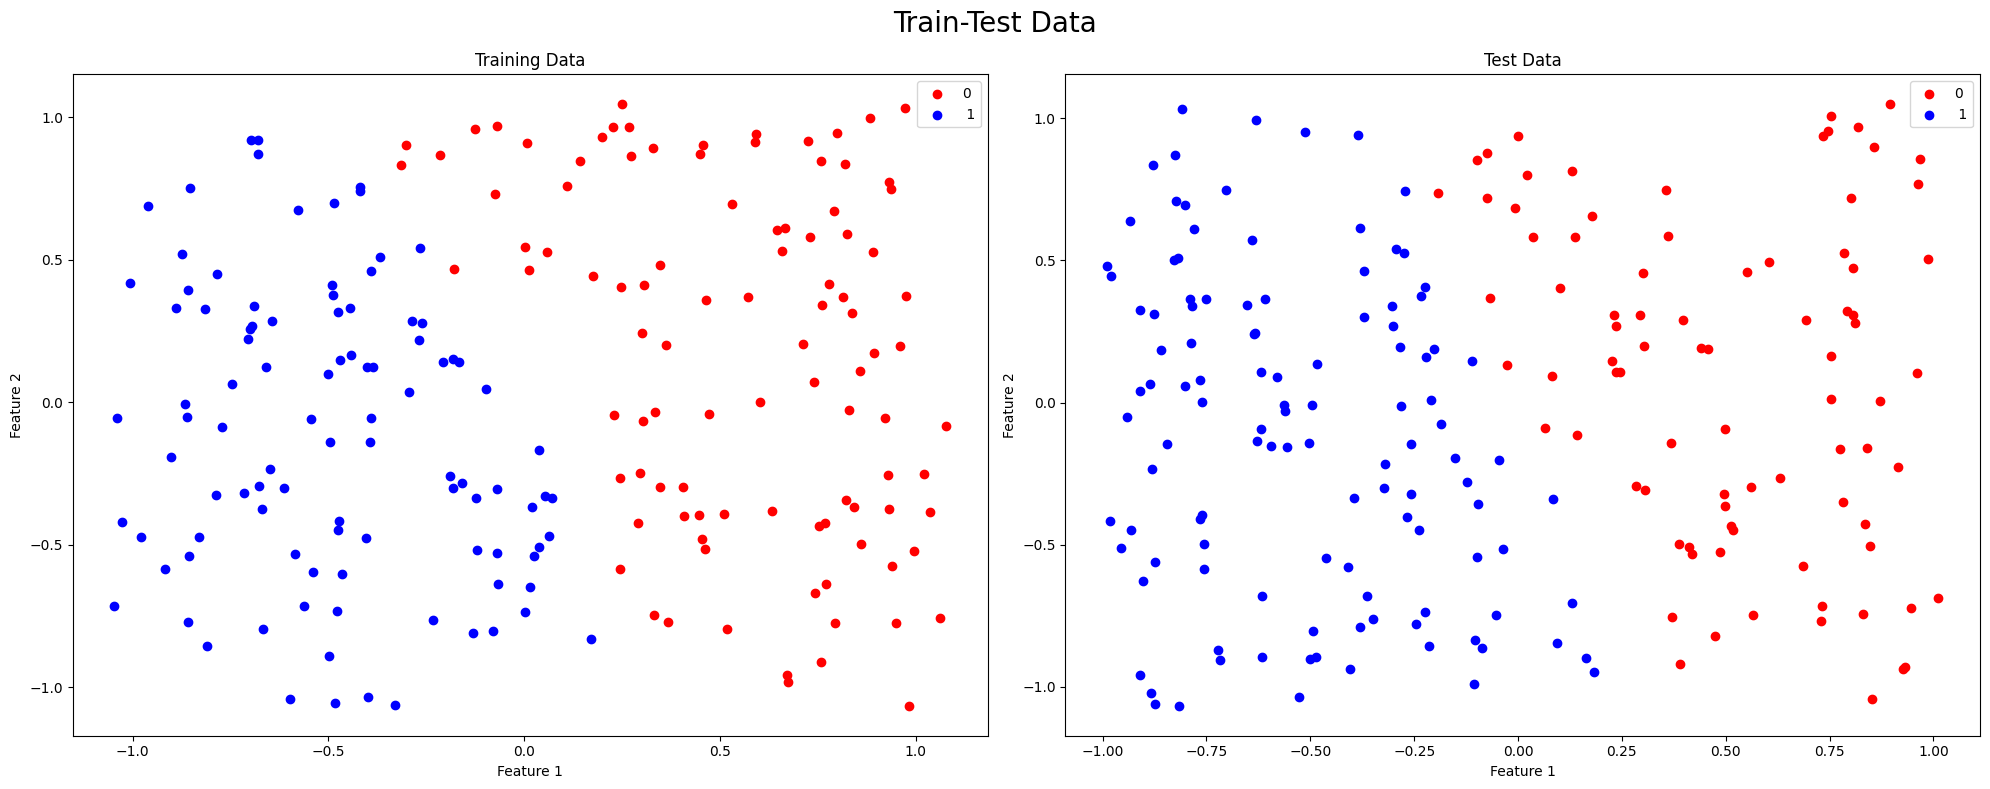
\includegraphics[width=0.7\textwidth]{plots/2_lineardataset.png}
    \caption{Linear separable dataset (train, test set with 200 points each)}
\end{figure}

\begin{lstlisting}[language=python]

dim_in, dim_out = x_train.shape[1], 2
hidden_neuron_list = [1]
activation_list = ['ReLU', 'Sigmoid']
opt_init = None
opt_loss = L2Loss()
mlp = MLP(dim_in, dim_out, hidden_neuron_list, activation_list, opt_init)
opt_optim = SGD(mlp)
----------------------------------------

Model Summary
-------------
Layer 1: Linear - A Dim: 2, Output Dim: 1, Parameters: 3
Layer 2: ReLU
Layer 3: Linear - A Dim: 1, Output Dim: 2, Parameters: 4
Layer 4: Sigmoid
Total Parameters: 7
\end{lstlisting}

\begin{figure}[H]
    \centering
    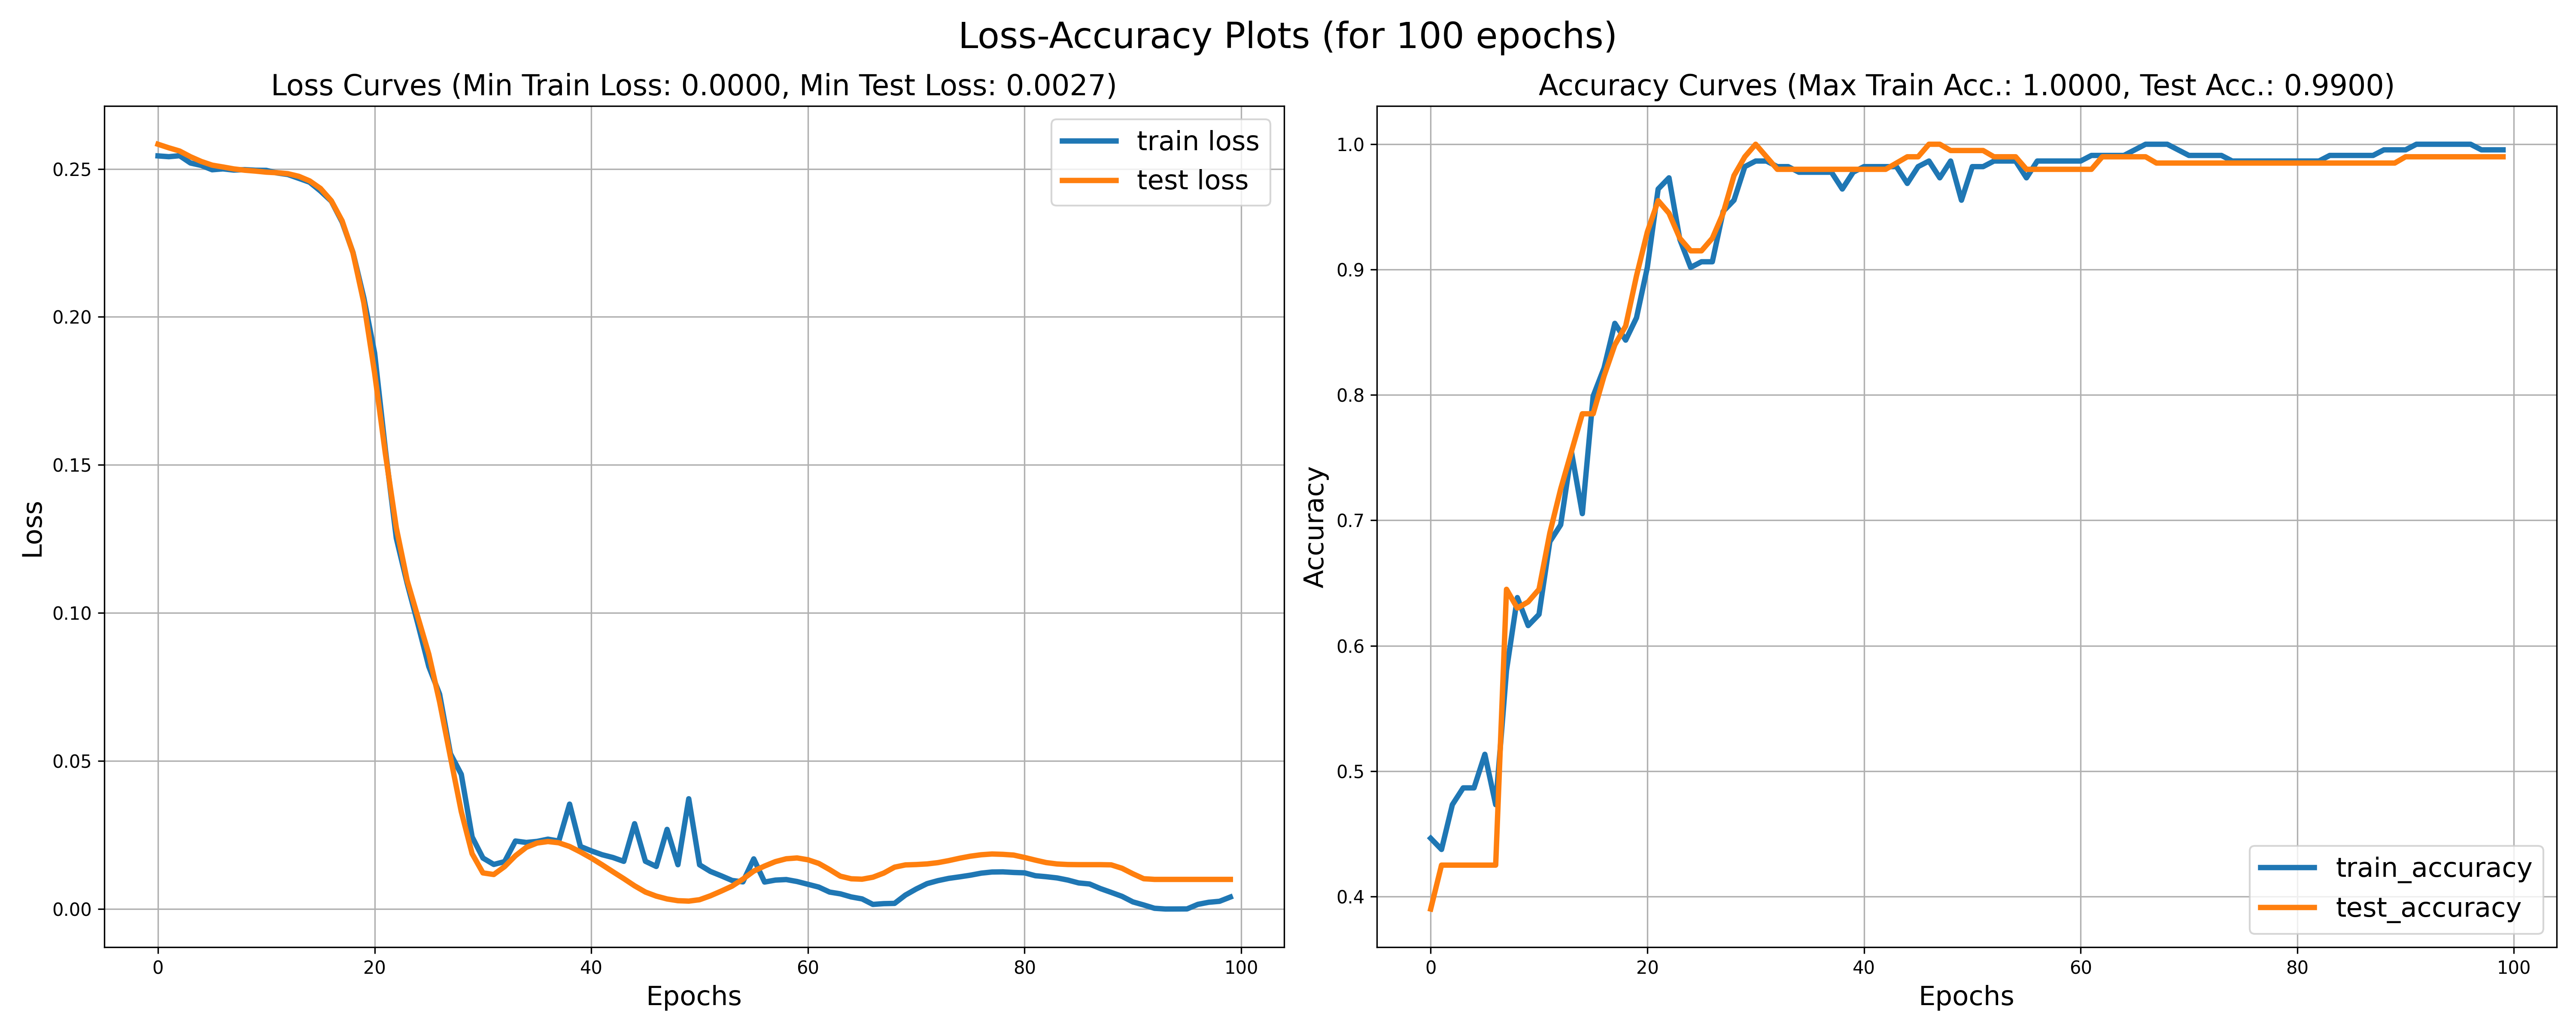
\includegraphics[width=0.8\textwidth]{plots/2_linearloss_acc.png}
    \caption{Loss and accuracy for linear separable dataset (train, test set with 200 points each)}
\end{figure}

\begin{figure}[H]
    \centering
    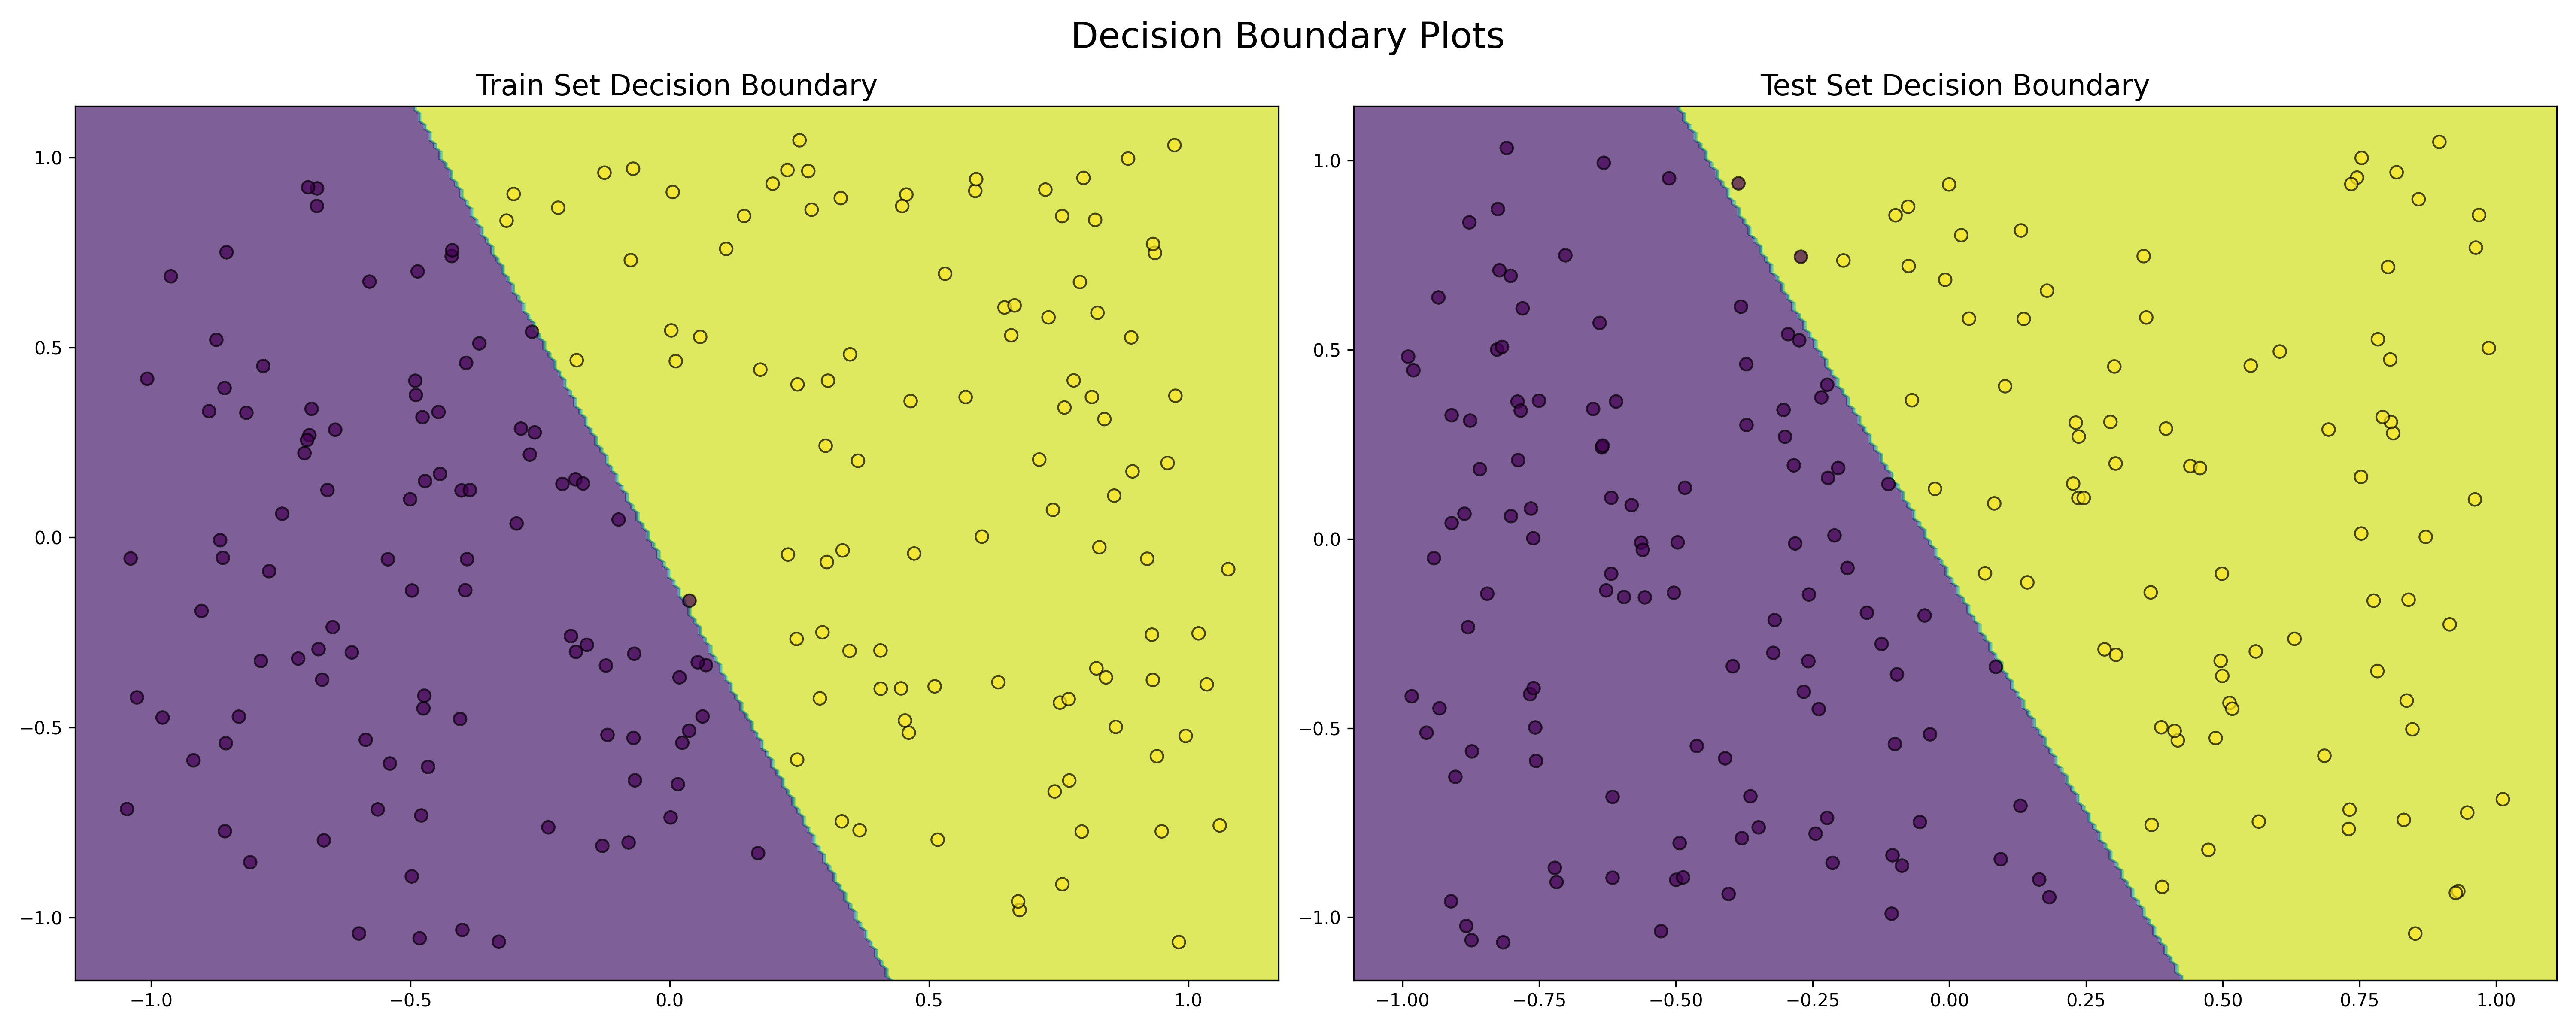
\includegraphics[width=0.7\textwidth]{plots/2_linearboundary.png}
    \caption{Decision boundary for linear separable dataset (train, test set with 200 points each)}
\end{figure}

\end{solve}

%%%%%%%%%%%%%%%%%%%%%%%%%%%%%%%%%%%%%%%%%%%%
\newpage
\section{Question 3}

\begin{itemize}
    \item  Create the imbalance datasets with all ``0'' digits and only 1\% ``1'' digits
    \item  Implement the training loop and evaluation section (implementing the $F_1$ metric)
    \item Ignore the class imbalance problem and train the MLP. Report your hyper-parameter details
    and the $F_1$ score performance on the test set (as the baseline)
    \item Explore modifications to improve the performance of the class imbalance problem. Report
    your modifications and the $F_1$ scores performance on the test set.
    \item Can you propose new ways for the class imbalance problem and achieve stable and satisfactory performance for large N = 500, 1000, $\dots$?
\end{itemize}

\begin{solve}

    \textbf{
    Extra credit (exploring the performance of the network for large N is done with the small N of 100, look at the tables for more details) }

    Model used was the same as the one used in question 1 for binary classifciation.

    \begin{lstlisting}[language=python]
SimpleMLP(
  (fc1): Linear(in_features=784, out_features=4, bias=True)
  (activation): ReLU()
  (fc2): Linear(in_features=4, out_features=2, bias=True)
)
\end{lstlisting}

    \subsubsection{Creation of Imbalanced Dataset where we sample every $N^{th}$ point}
    
    \textbf{We vary N from 100, then from 250 to 2000 with increments of 250 each. Thus the list $N_{list}$ varies from 100, 250, 500,..., 2000}

    \begin{lstlisting}[language=python]
train_0_original = [data for data in mnist if data[1] == 0]
train_1_original = [data for data in mnist if data[1] == 1]

# List of Ns (we sample every Nth point from list of 1s)
N_list = [100] + [250*(i+1) for i in range(8)]

for N in N_list:
    train_0 = train_0_original.copy()
    train_1 =  train_1_original.copy()
    random.shuffle(train_1)
    train_1 = train_1[:len(train_1) // N]
    print(N, 'Train set (before sparsing)',
     len(train_0), len(train_1), len(train_1) + len( train_0) )

    # Split training data (1s)into training and validation sets
    train_1len = int(len(train_1) *.8)
    val_1len = len(train_1) - train_1len
    train1_set, val1_set = random_split(train_1, [train_1len, val_1len])

    # Split training data (0s) into training and validation sets
    train_0len = int(len(train_0) *.8)
    val_0len = len(train_0) - train_0len
    train0_set, val0_set = random_split(train_0, [train_0len, val_0len])

    # combining 0 and 1s to get train and val sets
    train_set = train0_set + train1_set
    val_set = val0_set + val1_set
    len(train_set), len(val_set)

    # creating test set
    test_0 = [data for data in mnist_test if data[1] == 0]
    test_1 = [data for data in mnist_test if data[1] == 1]
    print(N,'Test set (before sparsing)',
    len(test_0), len(test_1), len(test_1) + len( test_0) )

    test_1 = test_1[:len(test_1) // N]
    print(N,'Test set (after sparsing)'
    ,len(test_0), len(test_1), len(test_1) + len( test_0) )
    test_set = test_0 + test_1
    print('\n')

    # Define DataLoaders to access data in batches
    train_loader = DataLoader(train_set, batch_size=64, shuffle=True)
    val_loader = DataLoader(val_set, batch_size = 64, shuffle=False)
    test_loader = DataLoader(test_set, batch_size = 64, shuffle=False)
    \end{lstlisting}
    

    \subsubsection{Implement $F_1$ metric}


\begin{lstlisting}[language=python, title= $F_1 Function$]
def precision_score(labels, predictions):
    predictions, labels = np.array(labels), np.array(predictions)
    predictions_1 = np.sum(predictions==1)
    correct_1 = np.sum( (predictions==1) & (labels==1))
    precision = correct_1/ predictions_1 if predictions_1 > 0 else 1e-6
    return precision

def recall_score(labels, predictions):
    predictions, labels = np.array(labels), np.array(predictions)
    correct_1 = np.sum( (predictions==1) & (labels==1))
    labels_1 = np.sum(labels==1)
    recall = correct_1/ labels_1 if labels_1 > 0 else 1e-6
    return recall

def f1_score(labels, predictions):
    precision = precision_score(labels, predictions)
    recall = recall_score(labels, predictions)
    f1 = (2 * (recall * precision)) / (precision + recall)
    return f1
\end{lstlisting}

Now we implement this in the val and test loops:
\begin{lstlisting}[language=python, title= Validation Loop]
# validation
val_loss = count = 0
correct = total = 0
val_preds = []; val_labels=[]
for data, target in val_loader:
    data, target = data.to(device), target.to(device)
    data = data.view(data.size(0), -1)
    output = model(data)
    val_loss += criterion(output, target).item()
    count += 1
    pred = output.argmax(dim=1)
    correct += (pred == target).sum().item()
    total += data.size(0)
    val_preds.append(pred)
    val_labels.append(target)
    # print(type(target))

# concat preds and true labels across all batches
val_preds = torch.cat(val_preds).numpy()
val_labels = torch.cat(val_labels).numpy()
assert len(val_preds) == len(val_set)

val_loss = val_loss / count
val_acc = 100. * correct / total
# print(f'Validation loss: {val_loss:.2f}, accuracy: {val_acc:.2f}%')
f1_validation = f1_score(labels = val_labels, predictions = val_preds)
# print(f'F1 score validation: {f1_validation:.2f}')
\end{lstlisting}

\begin{lstlisting}[language=python, title=Test Loop]
# test
model.eval()
correct = total = 0
test_preds = []; test_labels=[]

with torch.no_grad():
    for data, target in test_loader:
        data, target = data.to(device), target.to(device)
        data = data.view(data.size(0), -1)
        output = model(data)
        pred = output.argmax(dim=1)
        correct += (pred == target).sum().item()
        total += data.size(0)
        test_preds.append(pred)
        test_labels.append(target)

# concat preds and true labels across all batches
test_preds = torch.cat(test_preds).numpy() 
test_labels = torch.cat(test_labels).numpy()
assert len(test_preds) == len(test_set)   
test_acc = 100. * correct / total
# print(f'Test Accuracy: {test_acc:.2f}%')
# print(f'Validation loss: {val_loss:.2f}, accuracy: {val_acc:.2f}%')
f1_test = f1_score(labels = test_labels, predictions =test_preds)
# print(f'F1 score test: {f1_test:.2f}')
\end{lstlisting}




\subsubsection{Analysis of the model performance for different degrees of sparsity (larger N means more sparse dataset)}

\textbf{Structure:} 

For testing the performance, we use two different data sets. One is the original (unsparsed test dataset), the other sparsed data set (where we sample every Nth datapoint). The model is trained and validated on the sparse datasets but we test on the different datasets.

\begin{enumerate}
    \item {Performance on sparsed test data}
    
    \begin{figure}[H]
        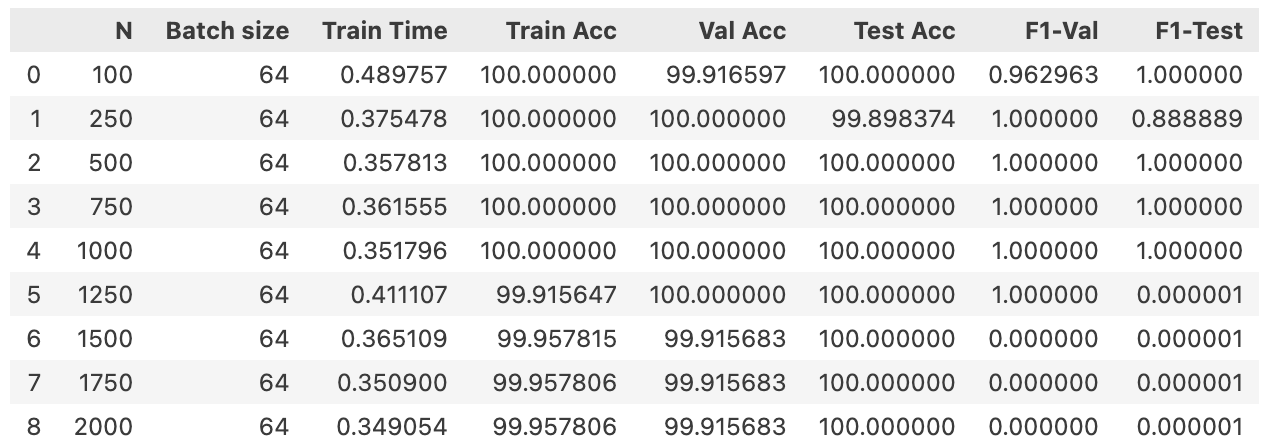
\includegraphics[scale=.7]{plots/No_mods.png}
        \caption{no modifications, test: sparsted data where N shows every Nth data point from the train, validation, and test datasets were sampled}
        \label{no_mods}
    \end{figure}

    \item {Performance on original/unsparsed test data}
    \begin{figure}[H]
        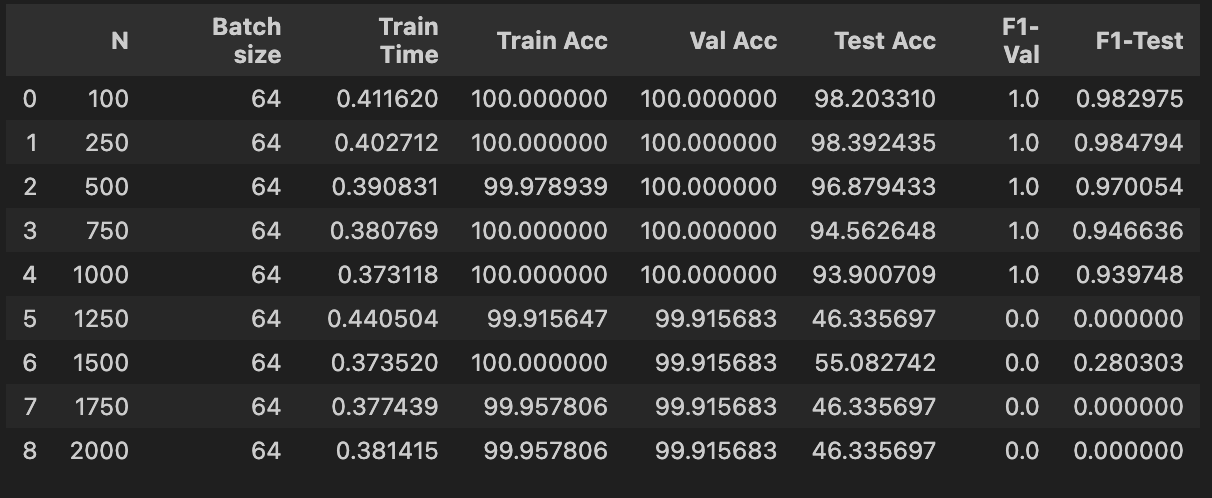
\includegraphics[scale=.7]{plots/No_mods_unsparsed.png}
        \caption{no modifications, here N shows every Nth data point from the train, validation were sampled. Test data remained unchanged}
        \label{no_mods_og}
    \end{figure}

    \item {Observations}
    We see that the model despite sparsity in Fig~\ref{no_mods} that eveen for sparsity of upto 1000, the model does really well in terms of $F_1$ score. $N=250$ is an exception but it was just this specific run, meaning pictures that model found hard were selected which increased the average loss count compared to other runs. 

    Despite having a very different distribution to the train and validation, in the case of the original unsparsed test data, we see in Fig~\ref{no_mods_og} that the $F_1$ score is lesser (which is what we would expect given it no more follows the sparsed dataset distribution that our model is trained on). However, it is still acceptable for $N=750$ hovering around $.95$. 

    In both cases, we see that for $N>1000$, the $F_1$ score drops considerably. In the case of sparsed dataset it drops down to $0$ because there is no $1$ in the test dataset. In the case of original dataset too we see a drop, that is somehow back up again for $N=1500$. 

    Thus, we see a huge bottle neck for the two methods at the 1000 threshold.
\end{enumerate}



\subsubsection{Adjusted Class Weights in the Loss Function: Aalysis of the model performance for different degrees of sparsity for different loss weights}

\textbf{Structure:} 

For testing the performance, we use two different data sets. One is the original (unsparsed test dataset), the other sparsed data set (where we sample every Nth datapoint). The model is trained and validated on the sparse datasets but we test on the different datasets.

\begin{lstlisting}[language=python, title = Adjusting the weight in the loss function]
# reweight_factor = weight[1]/ weight[0] 
model = SimpleMLP(in_dim=28 * 28,
hidden_dim=hidden_dim,
out_dim=2).to(device)
criterion = nn.CrossEntropyLoss(weight = weight)
optimizer = torch.optim.Adam(model.parameters(), lr=1e-2)
num_epochs = 10
\end{lstlisting}

In the table, the $Weight$ means how much more the sparse class (\textbf{1}) was over weighted in the loss function in comparsion to $0$. 

For each of the $N$, four different weights were tried:
$\left[1, \frac{N}{10}, \frac{N}{2}, \frac{len(train 0)}{len(train 1)}\right]$

\begin{enumerate}
    \item {Performance on sparsed test data}
    
    \begin{figure}[H]
        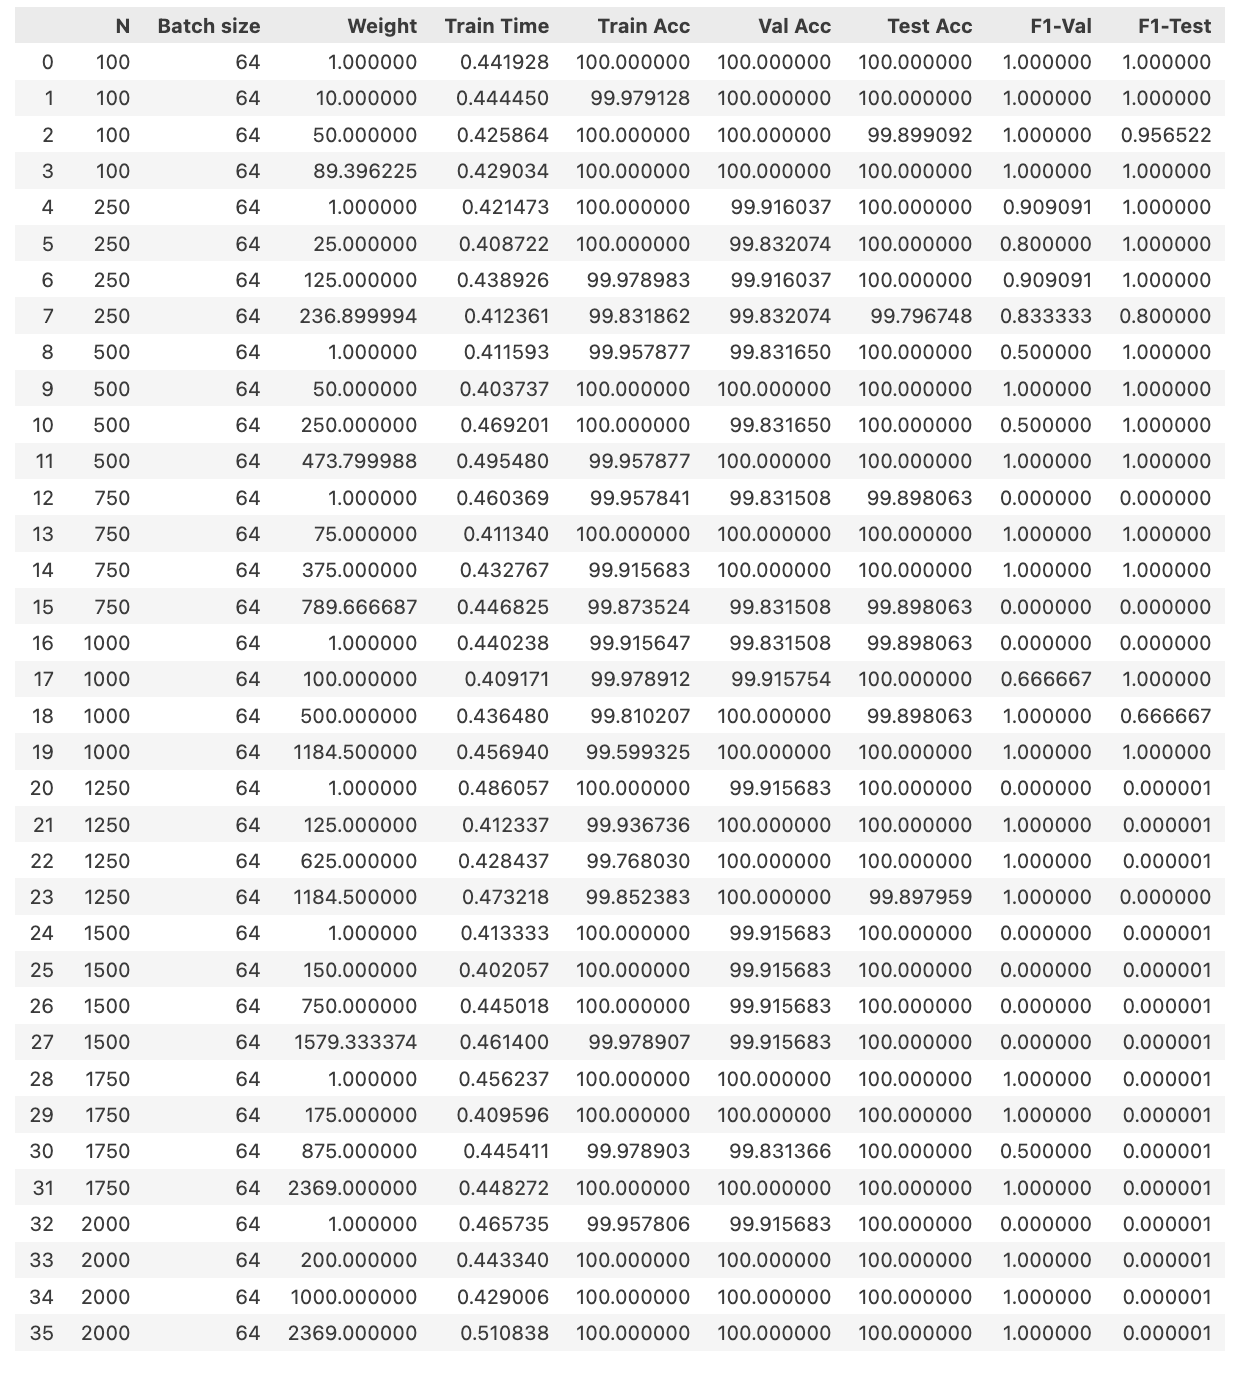
\includegraphics[scale=.72]{plots/2_weight_sparsed.png}
        \caption{Adjusted Class weights in the  Loss Function, test: sparsted data where N shows every Nth data point from the train, validation, and test datasets were sampled}
        \label{weight_mod_on_sparsed_test}
    \end{figure}

    \item {Performance on original/unsparsed test data}
    \begin{figure}[H]
        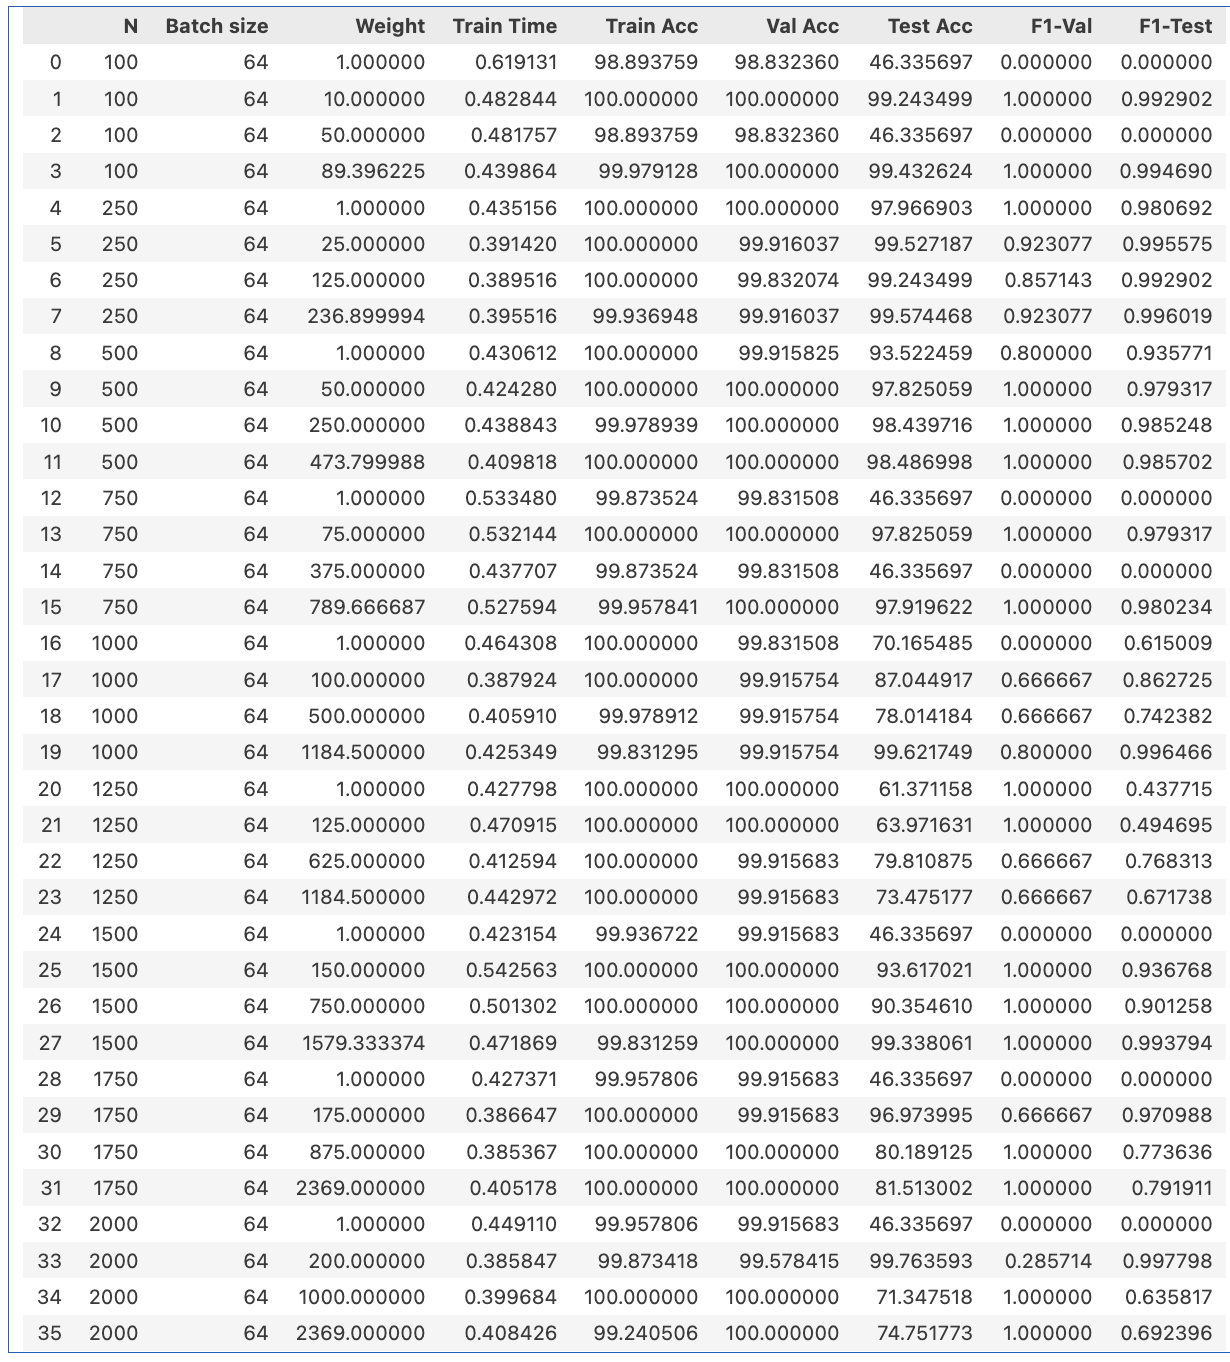
\includegraphics[scale=.72]{plots/2_weight_og.png}
        \caption{Adjusted Class weights in the  Loss Function, test: sparsted data where N shows every Nth data point from the train, validation. Test datasets was left as original test data set}
        \label{weight_mod_on_unsparsed_test}
    \end{figure}

    \item {Observations}
    
    Across both the sparsed and the unsparsed dataset we see huge improvements in the $F_1$ scores for the validation dataset, which shows that the weighting works well. We note  that the weight of $1$ for each class does as expected (from previous Fig~\ref{weight_mod_on_sparsed_test} till $N=750$. But it drops down to 0 at $N\geq 1000$, because there is no data point belonging to 1 class in test dataset.

    We also note that in  Fig~\ref{weight_mod_on_sparsed_test}, higher weights of $ \frac{N}{10}, \frac{len(train 0)}{len(train 1)}$ for the sparse classes do decently well for $N=1000$. They suffer the same problem for $N>1000$ because the test set has no $1s$

    Despite having a very different distribution to the train and validation, in the case of the original unsparsed test data, we see in Fig~\ref{weight_mod_on_unsparsed_test} that the $F_1$ score is lesser for Ns upto 1000 (which is what we would expect given it no more follows the sparsed dataset distribution that our model is trained on). However, we see that the higher weights do decently well till $1500$. Beyond that we see that the best performing weight of $\frac{len(train 0)}{len(train 1)}$ becomes too large for it to do well, and we see the $ \frac{N}{10}$ weight factor does better with the $F_1$ score for test. 

\end{enumerate}


\subsubsection{Resampling in the Data Loader: Aalysis of the model performance for different degrees of sparsity for different resampling weights }

\textbf{Structure:} 

For testing the performance, we use two different data sets. One is the original (unsparsed test dataset), the other sparsed data set (where we sample every Nth datapoint). The model is trained and validated on the sparse datasets but we test on the different datasets.

\begin{lstlisting}[language=python, title = Adjusting the weight in the loss function]
train_set = train0_set + train1_set
val_set = val0_set + val1_set
random.shuffle(train_set)
random.shuffle(val_set)
len(train_set), len(val_set)

# creating test set
test_0 = [data for data in mnist_test if data[1] == 0]
test_1 = [data for data in mnist_test if data[1] == 1]
test_1 = test_1[:len(test_1) // N] # comment this out for the unsparsed
test_set = test_0 + test_1

test_loader = DataLoader(test_set, batch_size=64, shuffle=False)

compensation = int(train_0len/ train_1len)
weight_factors = [1, int(N/10), int(N/2), compensation]
batch_size = 64
results = []

for weight_factor in weight_factors:
    weights = np.array( [1.0 if data[1] == 0 
    else weight_factor for data in train_set])
    weights = torch.from_numpy(weights)
    sampler = WeightedRandomSampler(weights, num_samples=len(weights), 
    replacement=True)
    train_loader = DataLoader(train_set, batch_size=64, sampler=sampler)
    val_loader = DataLoader(val_set, batch_size=64, shuffle=False)
\end{lstlisting}

Note no shuffling in the false, this was inspired from \cite{No Shuffle}

In the table, the $Weight$ means how much more the sparse class (\textbf{1}) was over weighted in the loss function in comparsion to $0$. For each of the $N$, four different weights were tried:
$\left[1, \frac{N}{10}, \frac{N}{2}, \frac{len(train 0)}{len(train 1)}\right]$

\begin{enumerate}
    \item {Performance on sparsed test data}
    
    \begin{figure}[H]
        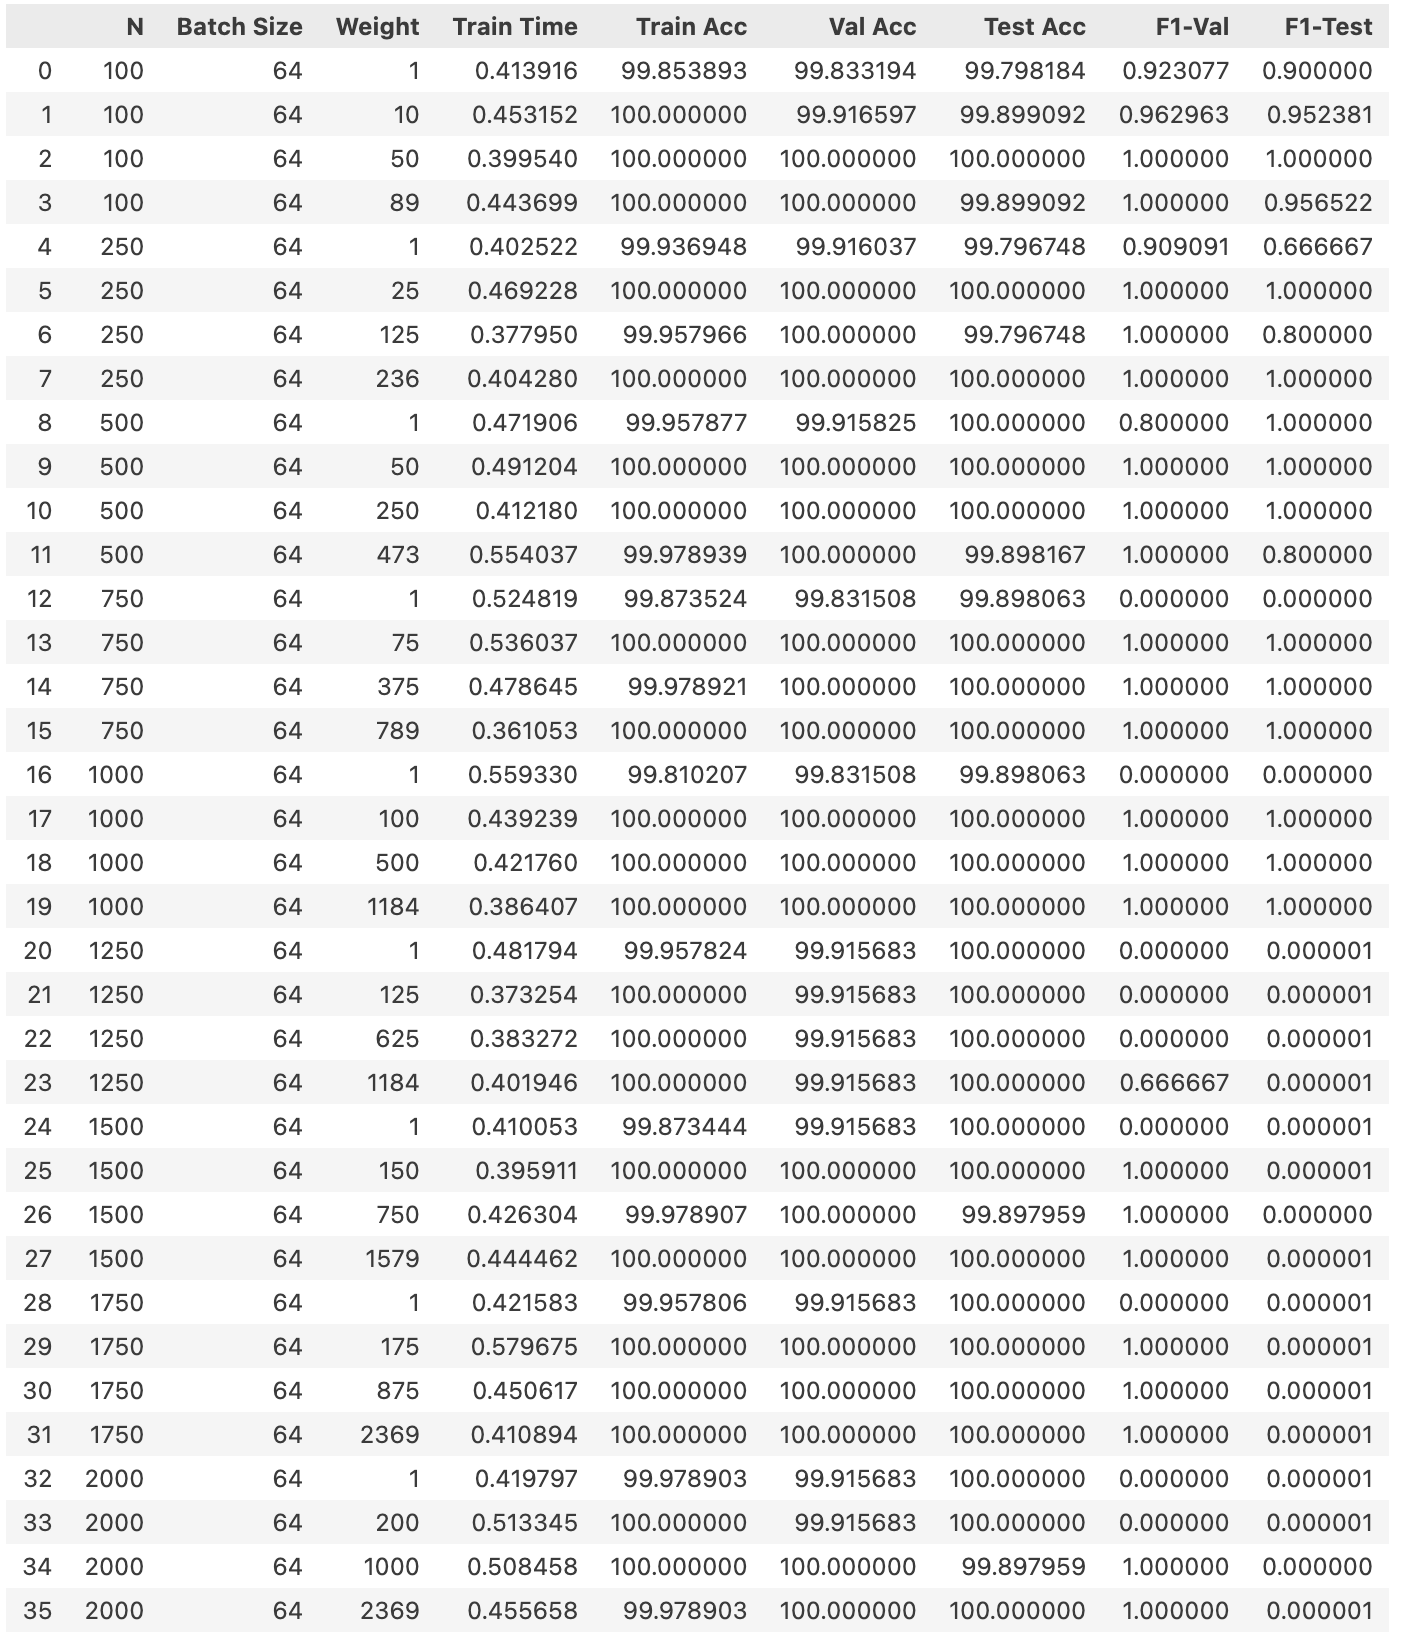
\includegraphics[scale=.7]{plots/resampling_on_sparsted_test.png}
        \caption{Adjusted Class weights in the  Loss Function, test: sparsted data where N shows every Nth data point from the train, validation, and test datasets were sampled}
        \label{resampling_sparsed_test}
    \end{figure}

    \item {Performance on original/unsparsed test data}
    \begin{figure}[H]
        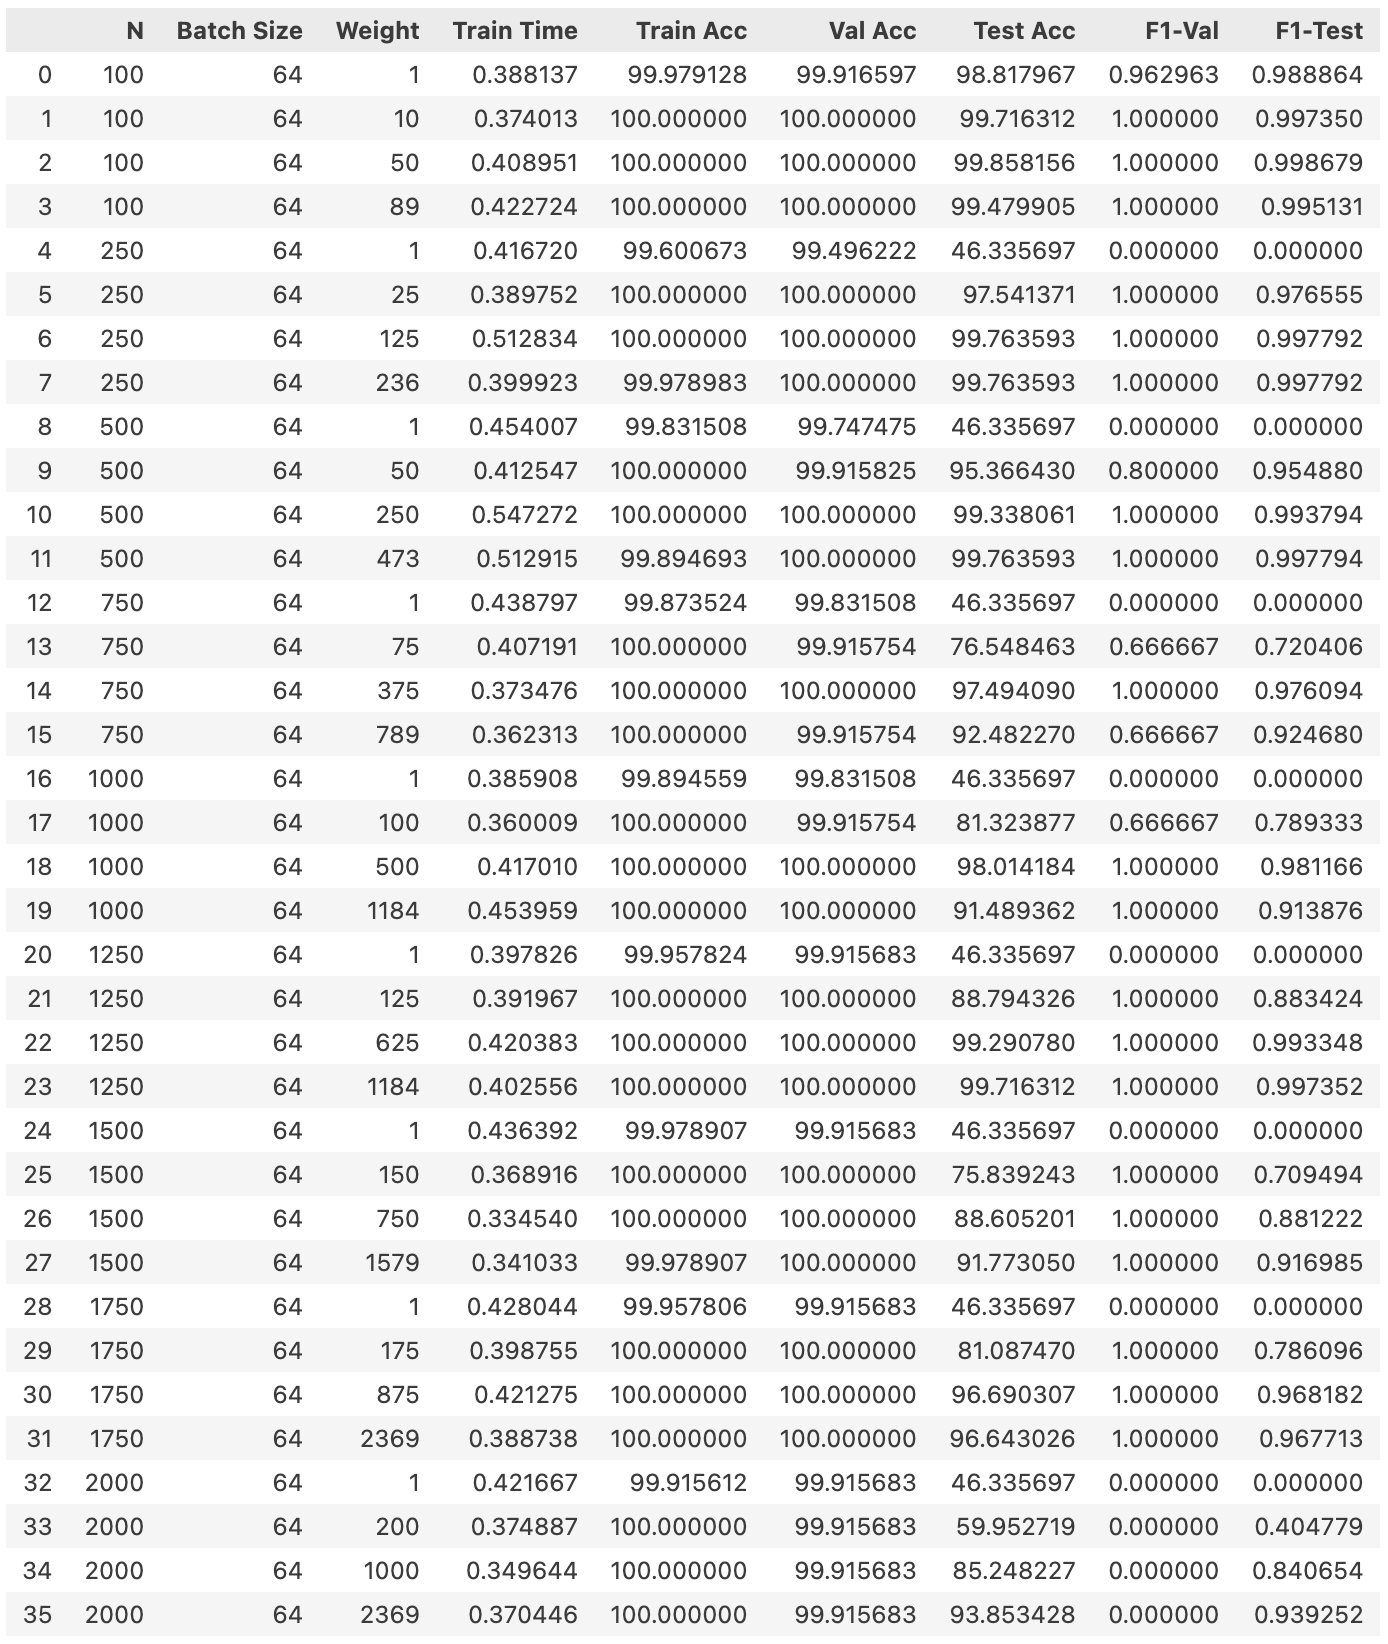
\includegraphics[scale=.7]{plots/resampling_on_unsparsed_test}
        \caption{Adjusted Class weights in the  Loss Function, test: sparsted data where N shows every Nth data point from the train, validation. Test datasets was left as original test data set}
        \label{resampling_unsparsed_test}
    \end{figure}

    \item {Observations}
    
    Across both the sparsed and the unsparsed dataset we see huge improvements in the $F_1$ scores for the validation dataset over no modifications, which shows that the resampling works well. We note that resampling for lower weights does better that adjusting weights in the loss.

    We also note that in  Fig~\ref{resampling_sparsed_test}, higher weights of for the sparse classes do decently well for $N=1000$. They suffer the same problem for $N>1000$ because the test set has no $1s$. However, over the weight adjustment for the loss function, we do not see a huge difference in the performance.

    However, we do see a decent difference in the performance in resampling over loss weighting for large Ns in Fig~\ref{resampling_unsparsed_test}. $N=1750$ offers a good comparison where we see the validation $F_1$ of 1 and test $F_1$ of around $.97$ for a factor of $\frac{len(train 0)}{len(train 1)}$, whereas we had a test validation of $~.80$ in the case of loss weighting. However, see that the validation score was very low for unsparsed split of $N=2000$, it might be that the validation set did not have a $1$ class. 

    However, see still see that the $F_1 (test)$ for $N=2000$ is still considerably good at $.94$.


\textbf{Remark:}
We note that both weighting in the loss function and resampling in the Data loader offer considerable improvement over no modificaiton in the case of both original and sparsed test data sets. However, we see that the performance of a weighting factor in the data loader through resampling is a lot more consistent across different Ns than the weighting factor in the loss function. In the loss fuction, weighting the highest weights start off well, but we see that their performance drops off for large Ns. The intermediate weighting factors of $\frac{N}{2}, \frac{N}{10}$ start to perform better for more sparse data. 

This makes sense given that weighting the loss by a very large number can make the optimization unstable as we weight a specific class a lot more in the optimization. On the other hand, resampling offers a smoother alternative to weighting the loss function, especially as the sparsity grows too large.

\end{enumerate}


\end{solve}
%%%%%%%%%%%%%%%%%%%%%%%%%%%%%%%%%%%%%%%%%%%%
\newpage

\section{Question 4}

%%%%%%%%%%%%%%%%%%%%%%%%%%%%%%%%%%%%%%%%%%%%
\newpage

\section{Deliverable 5: Differences in Optimizers (Sinusoidal dataset)}


\begin{solve}    

\begin{figure}[H]
    \centering
    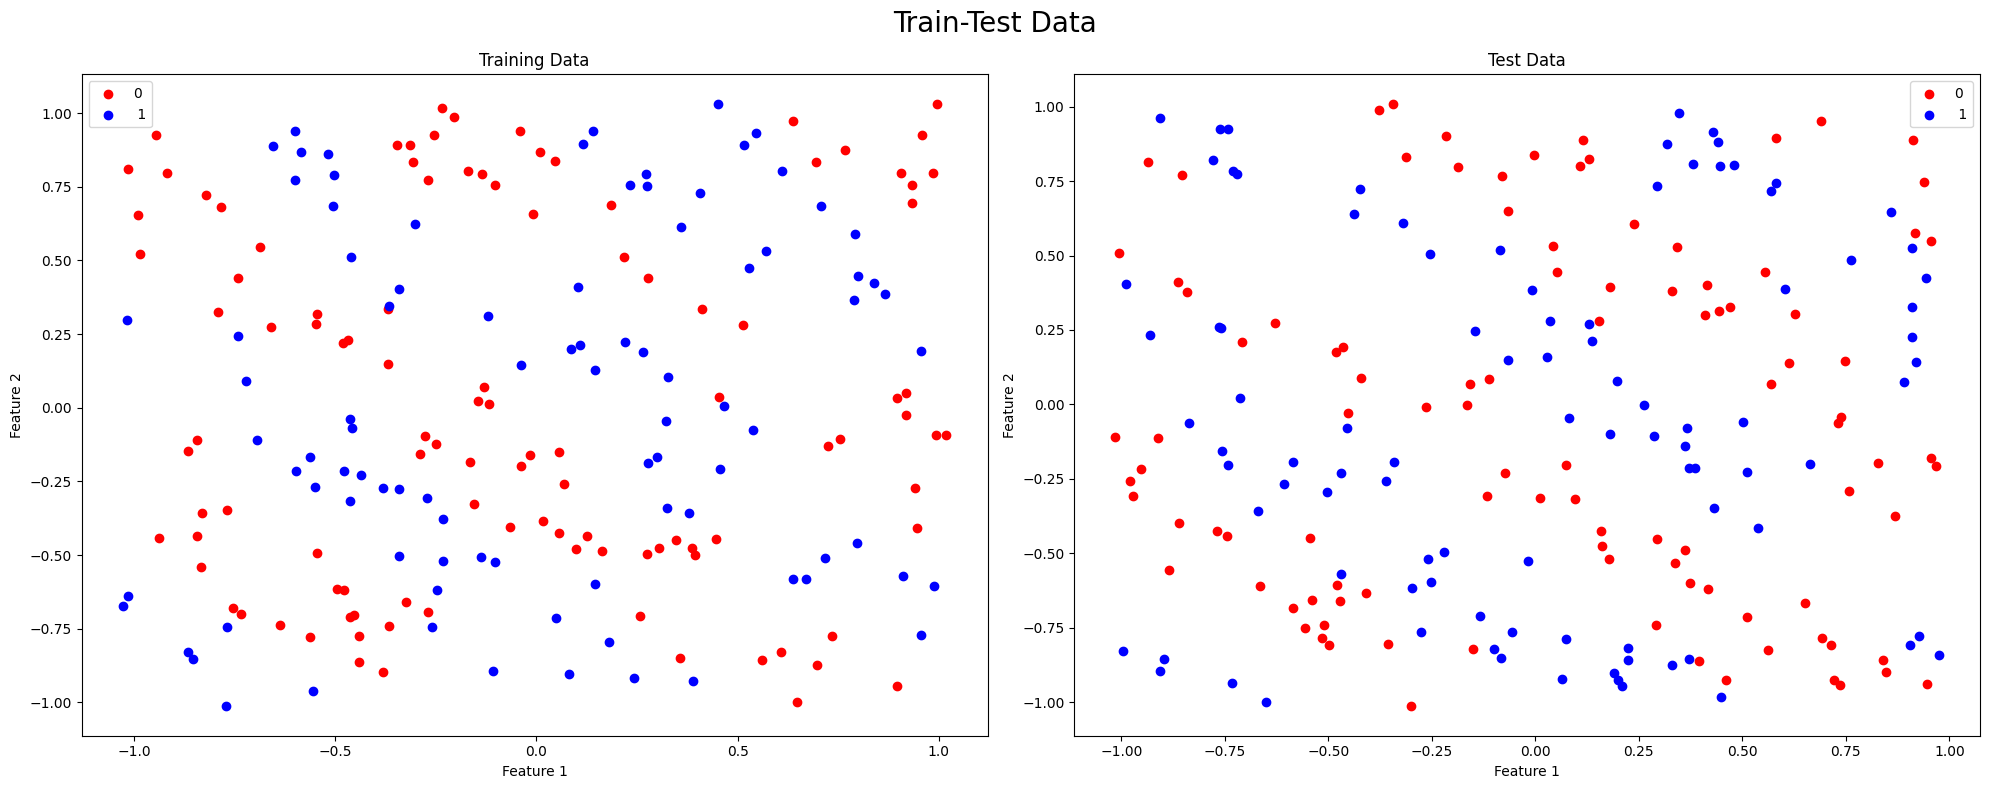
\includegraphics[width=0.7\textwidth]{plots/sinusoid_dataset.png}
    \caption{Sinusoidal dataset (train, test set with 200 points each)}
\end{figure}

\subsection*{Model Description}

\begin{lstlisting}[language=python]
dim_in, dim_out = x_train.shape[1], 2
hidden_neuron_list = [8, 16, 32, 8]
activation_list = ['ReLU','ReLU', 'ReLU','ReLU','LinearActivation'] 
# linear at the last layer because sigmoiding in the loss function forward pass for CrossEntropyLoss
opt_init = 'xavier'
opt_loss = CrossEntropyLoss()
mlp = MLP(dim_in, dim_out, hidden_neuron_list, activation_list, opt_init)
print(mlp.summary())
-----------------------------------------------------------------
Model Summary
-------------
Layer 1: Linear - A Dim: 2, Output Dim: 8, Parameters: 24
Layer 2: ReLU
Layer 3: Linear - A Dim: 8, Output Dim: 16, Parameters: 144
Layer 4: ReLU
Layer 5: Linear - A Dim: 16, Output Dim: 32, Parameters: 544
Layer 6: ReLU
Layer 7: Linear - A Dim: 32, Output Dim: 8, Parameters: 264
Layer 8: ReLU
Layer 9: Linear - A Dim: 8, Output Dim: 2, Parameters: 18
Layer 10: LinearActivation
Total Parameters: 994
    \end{lstlisting}


\subsection{Optimizer Performance}
We see that the Adam optimizer with learning rate 0.01 performs the best in terms of loss and accuracy. The decision boundary is also the most accurate. The performacne for the SGD optimizer with learning rate 0.01 and momentum is the second best (with lesser train accuracy but simlar test performance). We do see that tho the decision boundary is over fitting to train in this case.

Adam optimizer with learning rate 0.001 is lesser accurate, followed by vanilla SGD which gives the worst performance in terms of loss and accuracy. The decision boundary is also the most inaccurate.

\subsection{ \textcolor{red}{Best Performance: MLP with Adam Optimizer of learning rate 0.01 and default parameters} }

\begin{figure}[H]
    \centering
    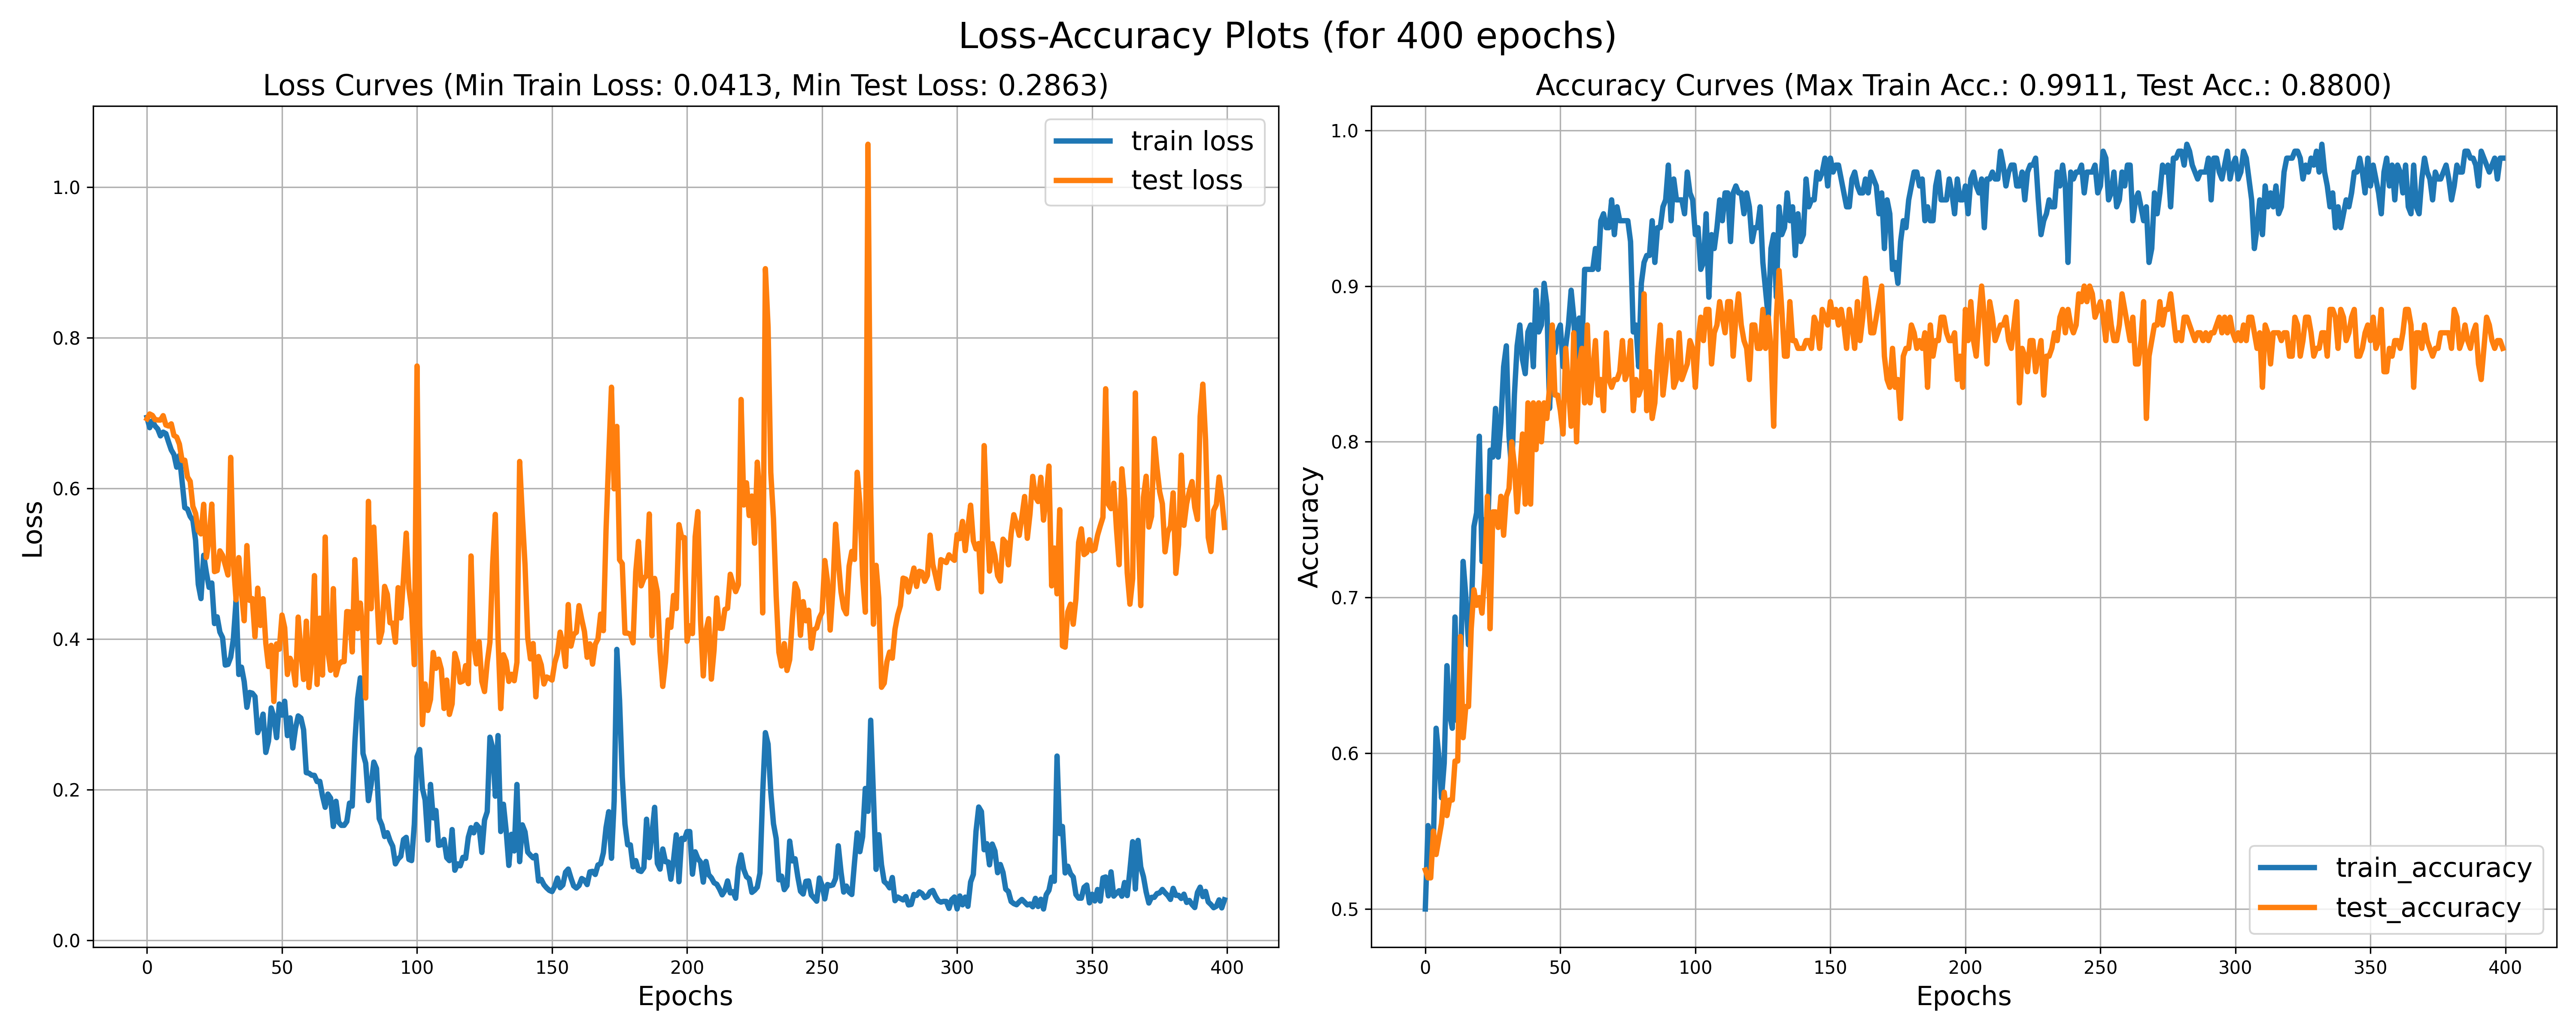
\includegraphics[width=0.9\textwidth]{plots/sinusoid_adam-lr1e-2_more_paramsloss_acc.png}
    \caption{Loss and accuracy for Circle dataset (train, test set with 200 points each)\\ Adam optimizer (lr $=1e-2$ ), 400 epochs, Cost function: CrossEntropyLoss, Xaiver initialization}
    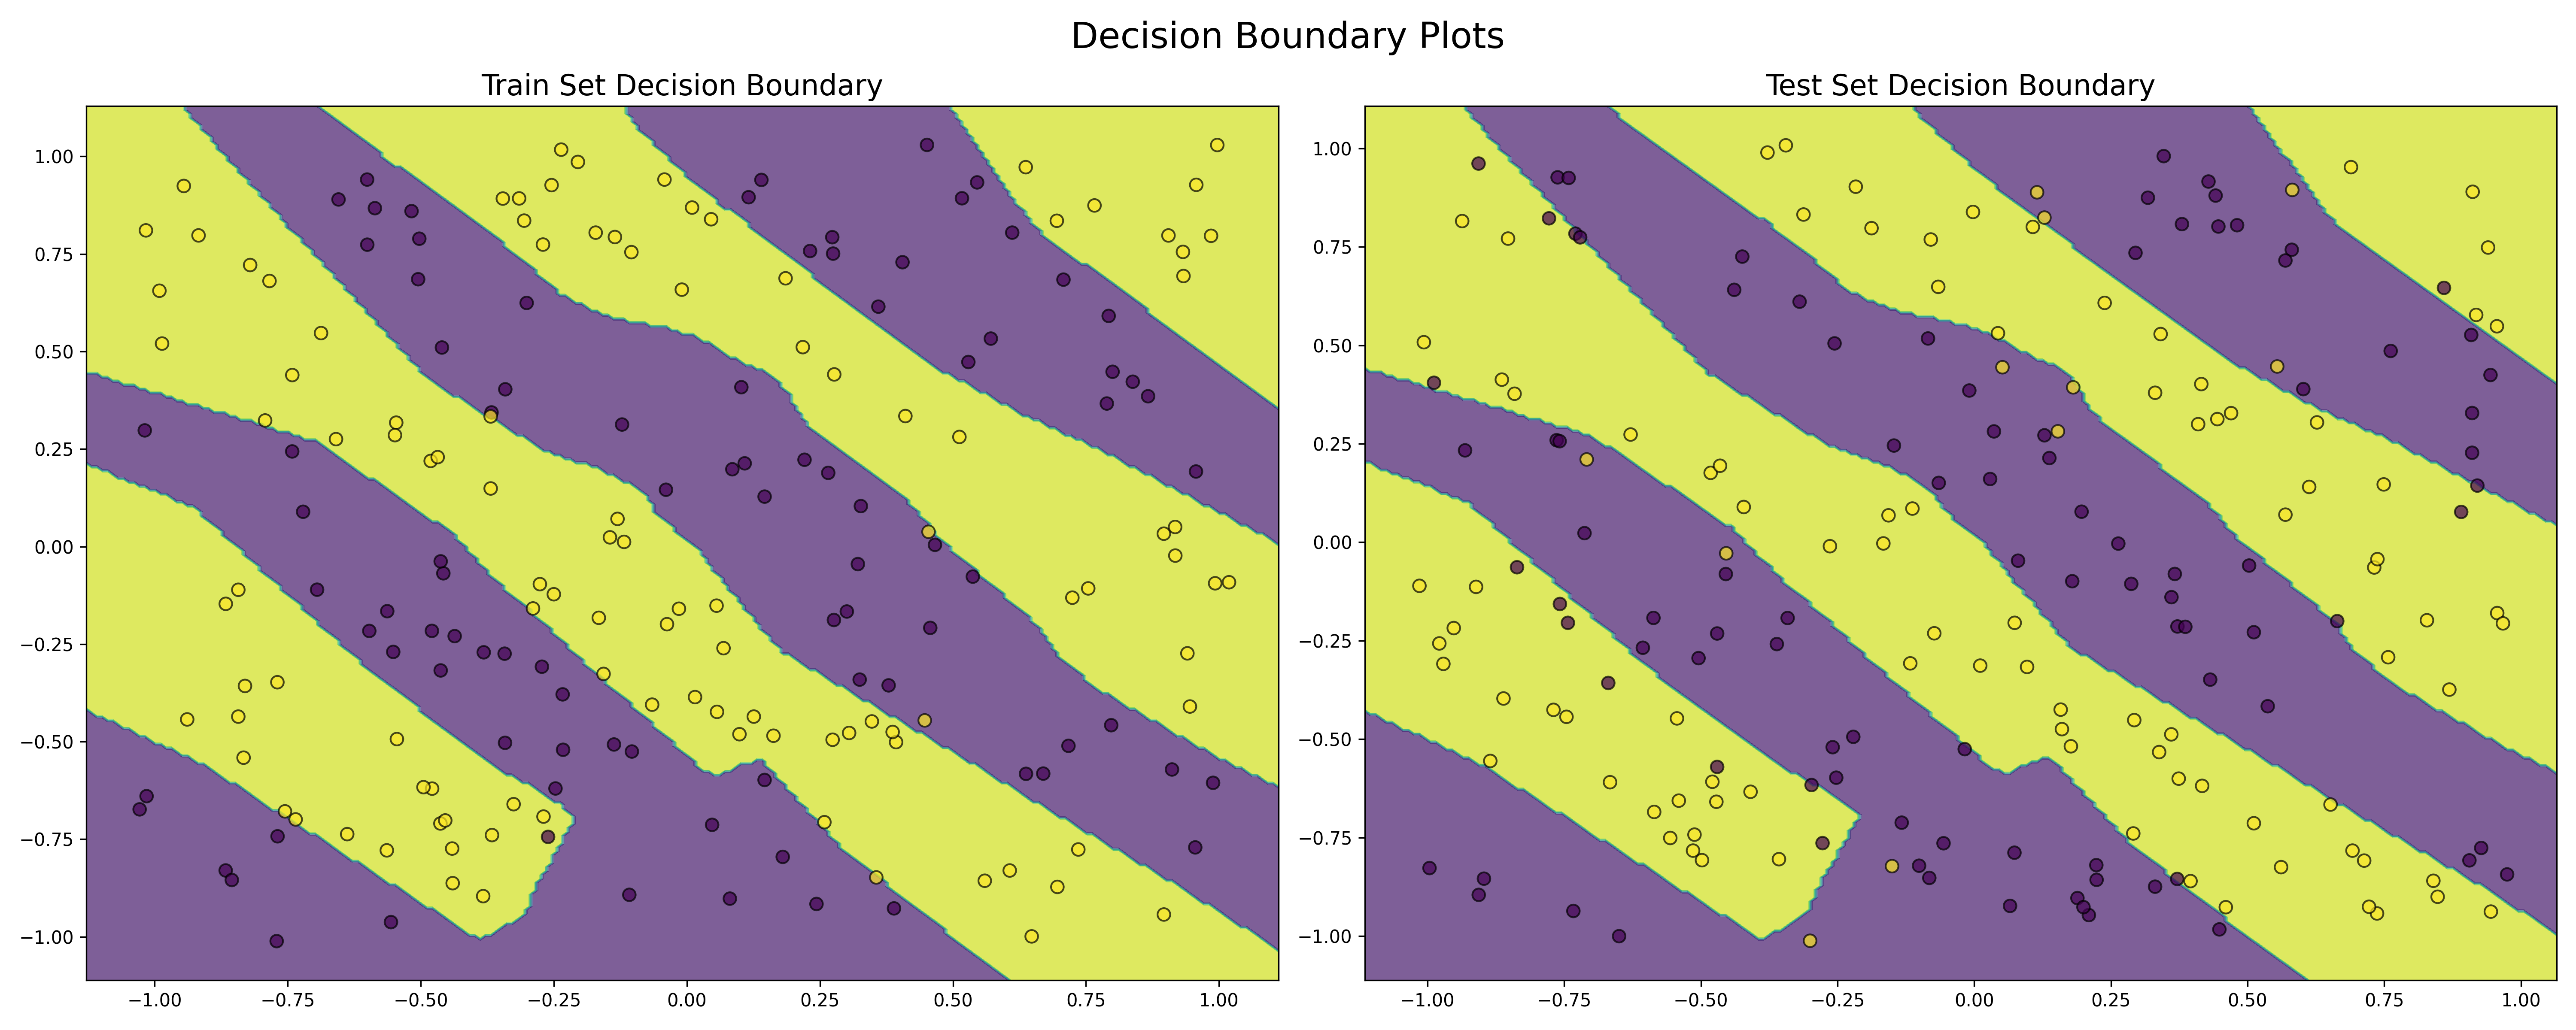
\includegraphics[width=0.8\textwidth]{plots/sinusoid_adam-lr1e-2_more_paramsboundary.png}
    \caption{(L2Loss) Decision boundary for Circle separable dataset (train, test set with 200 points each) 
    Adam optimizer (lr $=1e-2$ )}
\end{figure}

\subsection{MLP with SGD Optimizer of learning rate 0.01 and default parameters (no momentum, no weight decay)}

\begin{figure}[H]
    \centering
    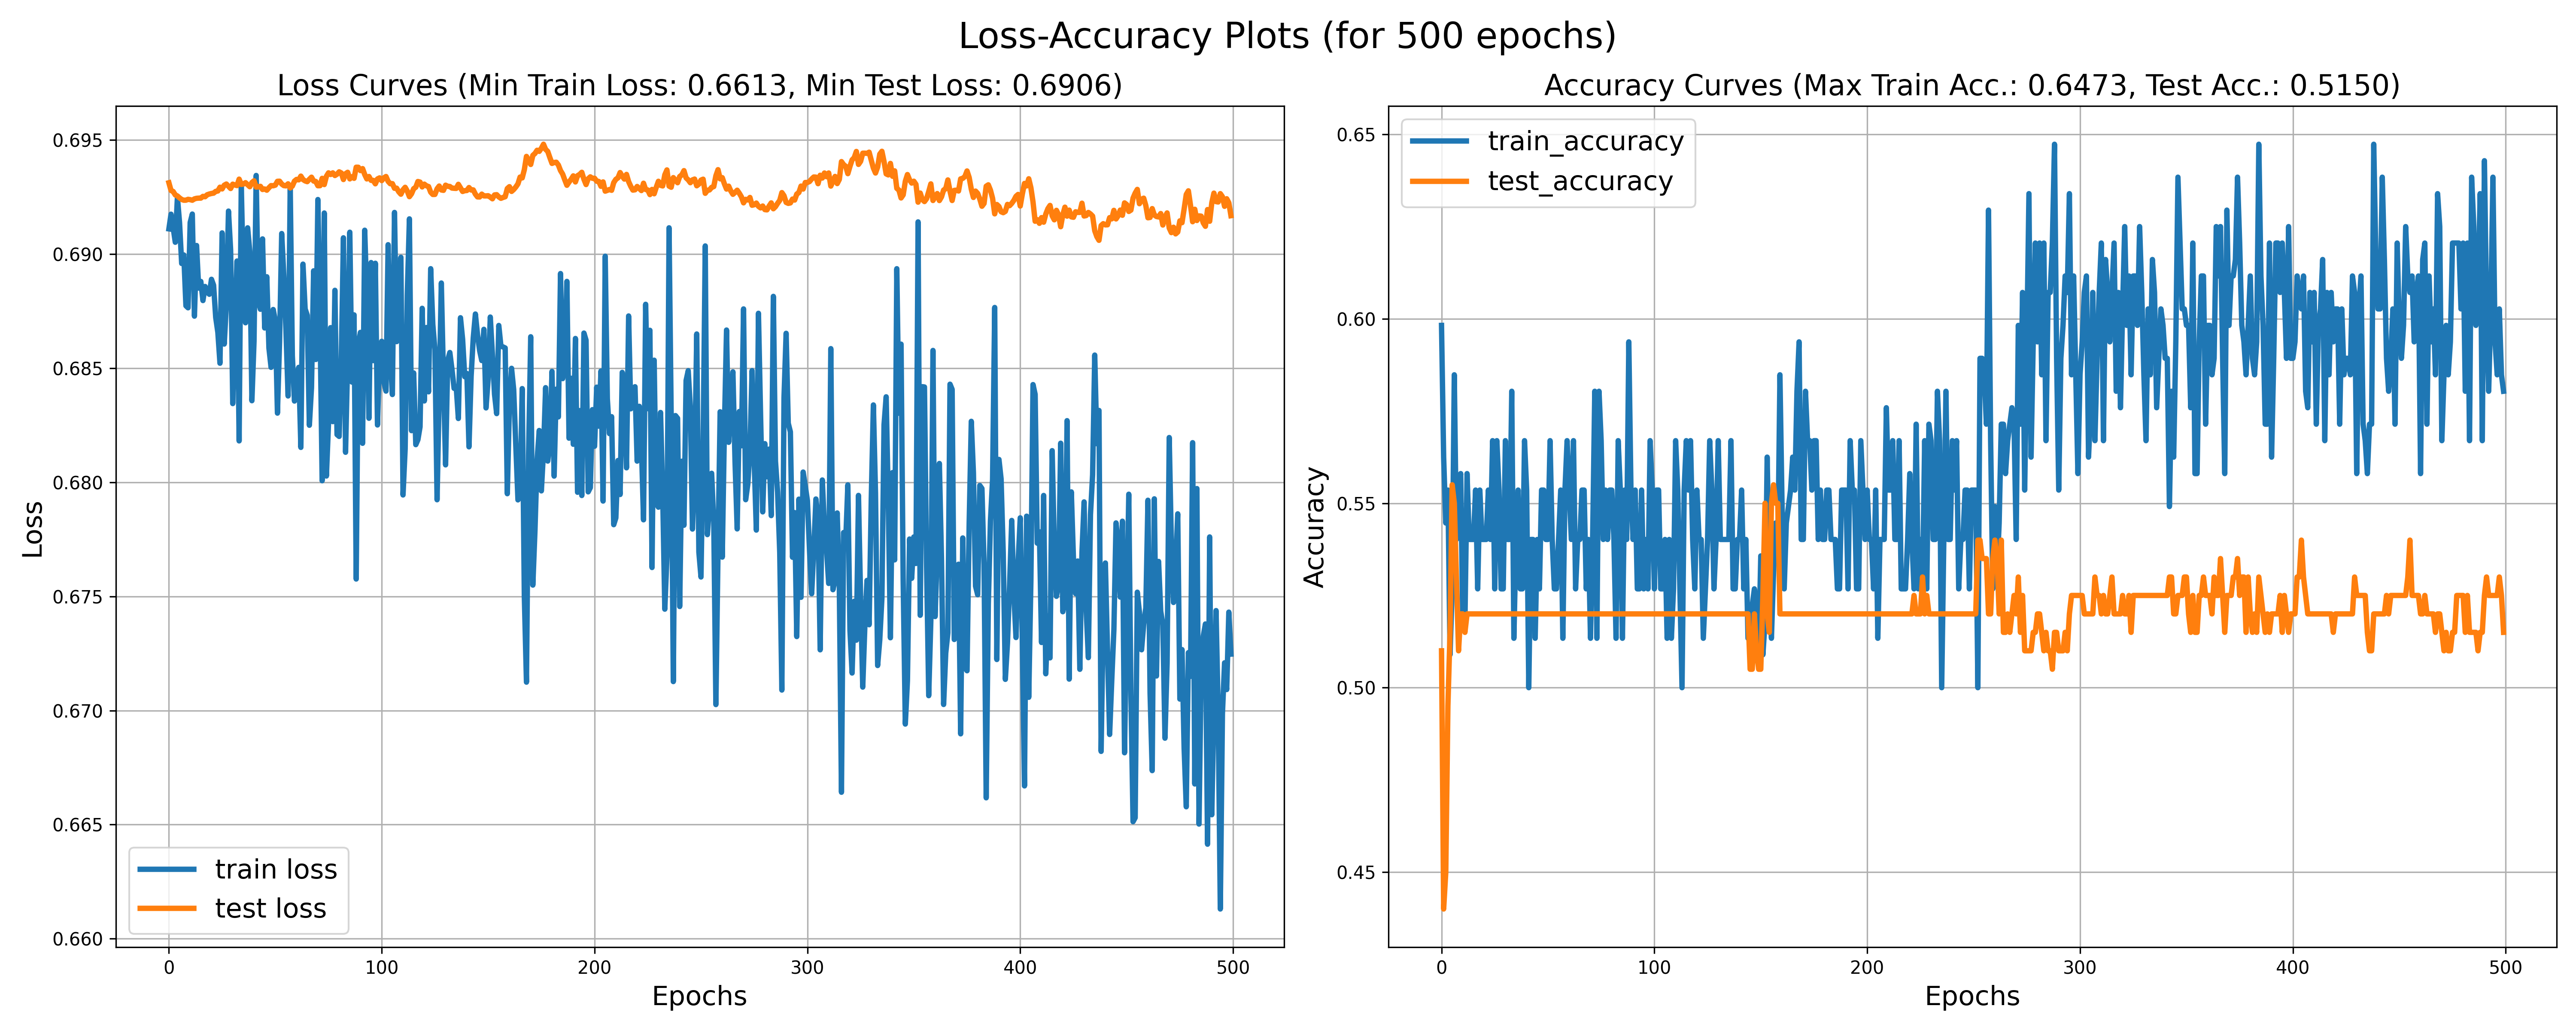
\includegraphics[width=0.9\textwidth]{plots/5_sinusoid_sgd_morelayers_loss_acc.png}
    \caption{Loss and accuracy for Circle dataset (train, test set with 200 points each)\\ SGD optimizer (lr $=1e-2$), 400 epochs, Cost function: CrossEntropyLoss, Xaiver initialization}
    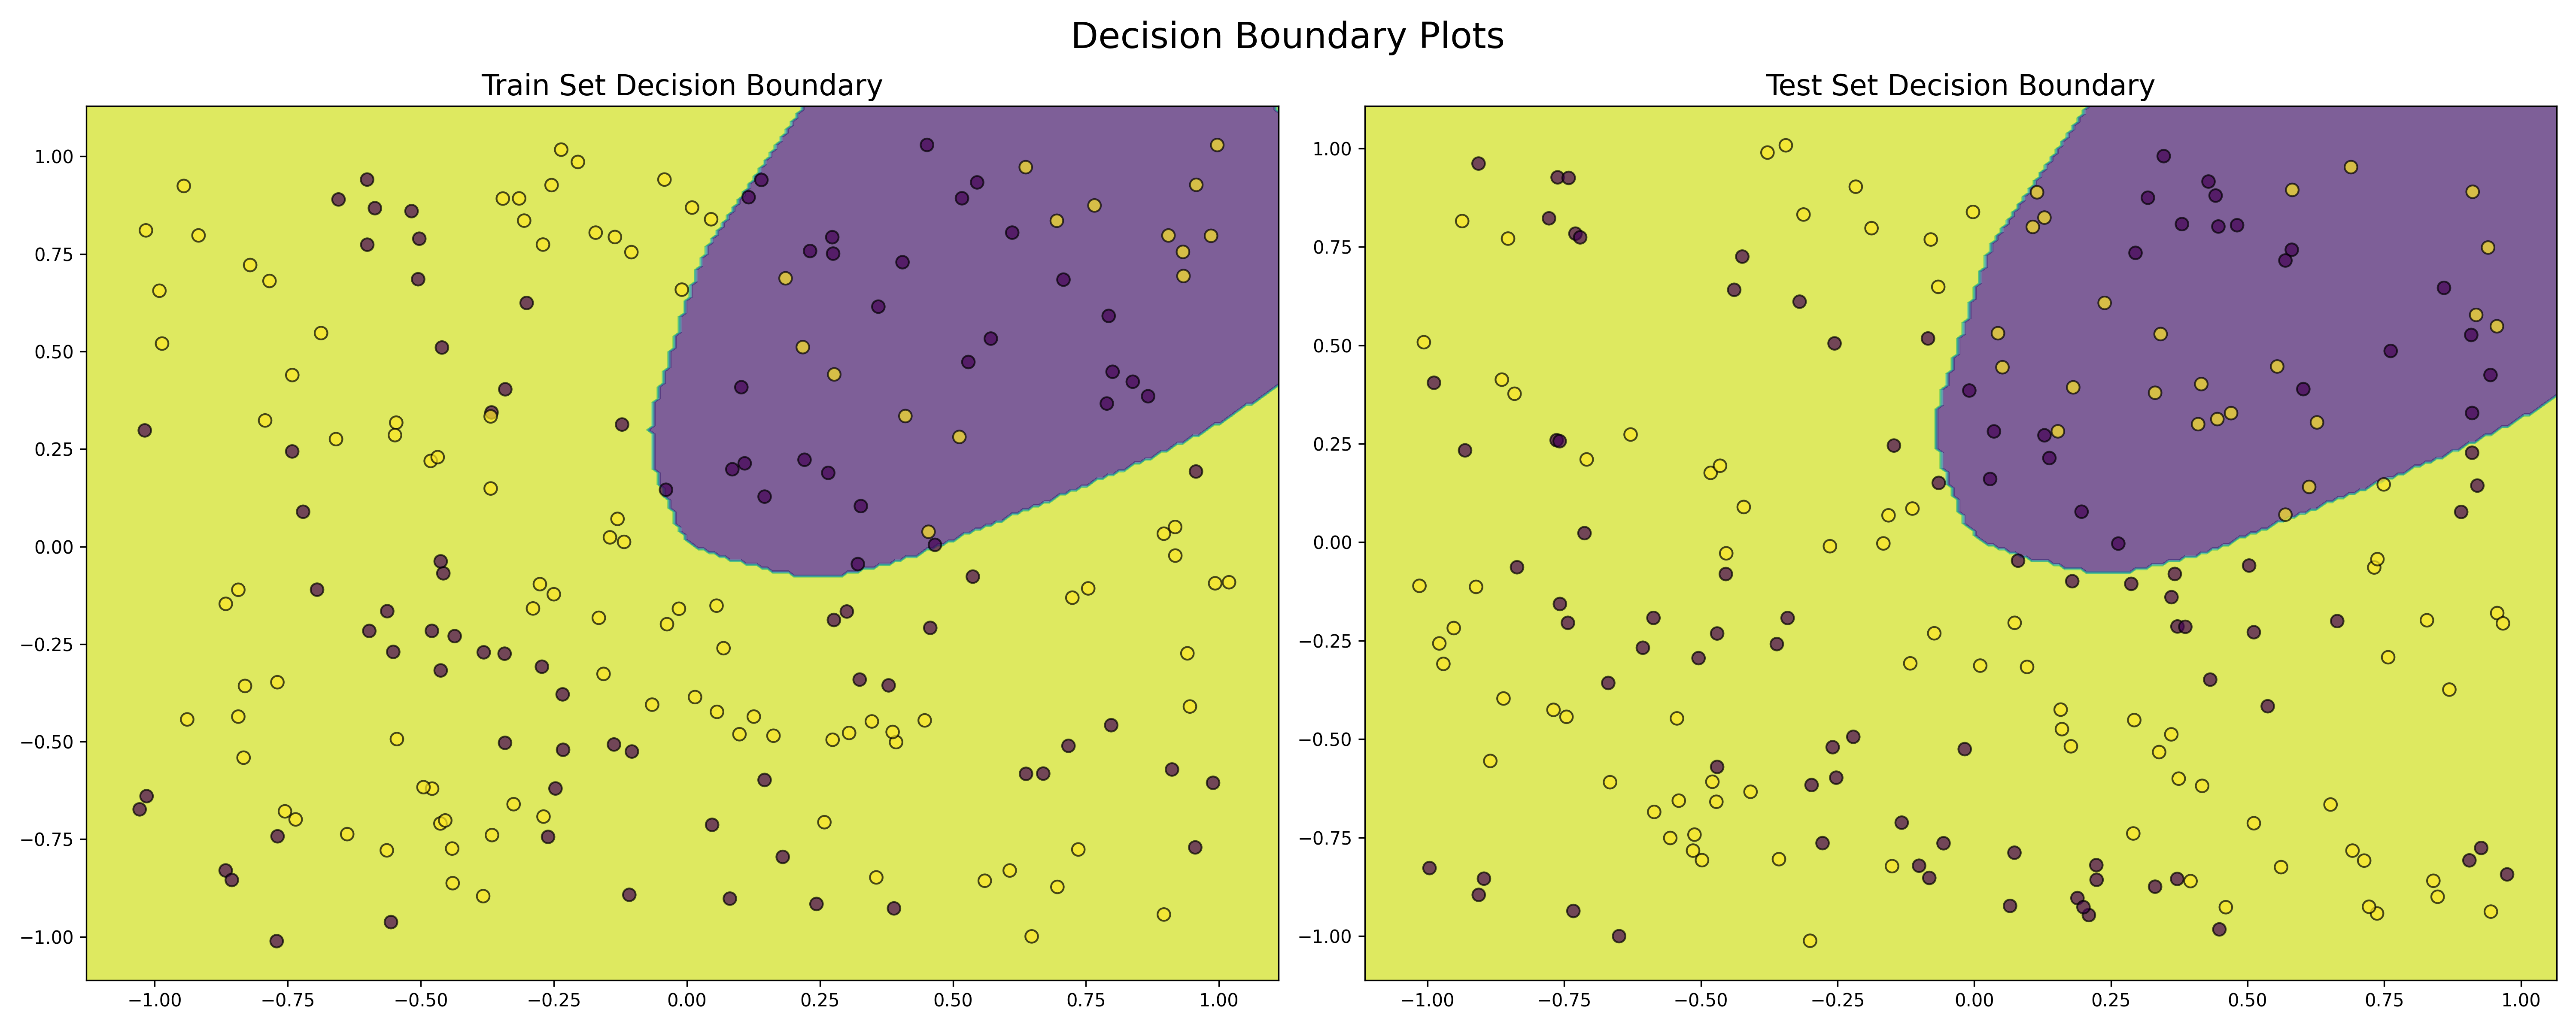
\includegraphics[width=0.8\textwidth]{plots/5_sinusoid_sgd_morelayers_boundary.png}
    \caption{(L2Loss) Decision boundary for Circle separable dataset (train, test set with 200 points each) 
    SGD (lr $=1e-2$ )}
\end{figure}

\subsection{MLP with SGD Optimizer of learning rate 0.01 momentum 0.9, no weight decay}

\begin{figure}[H]
    \centering
    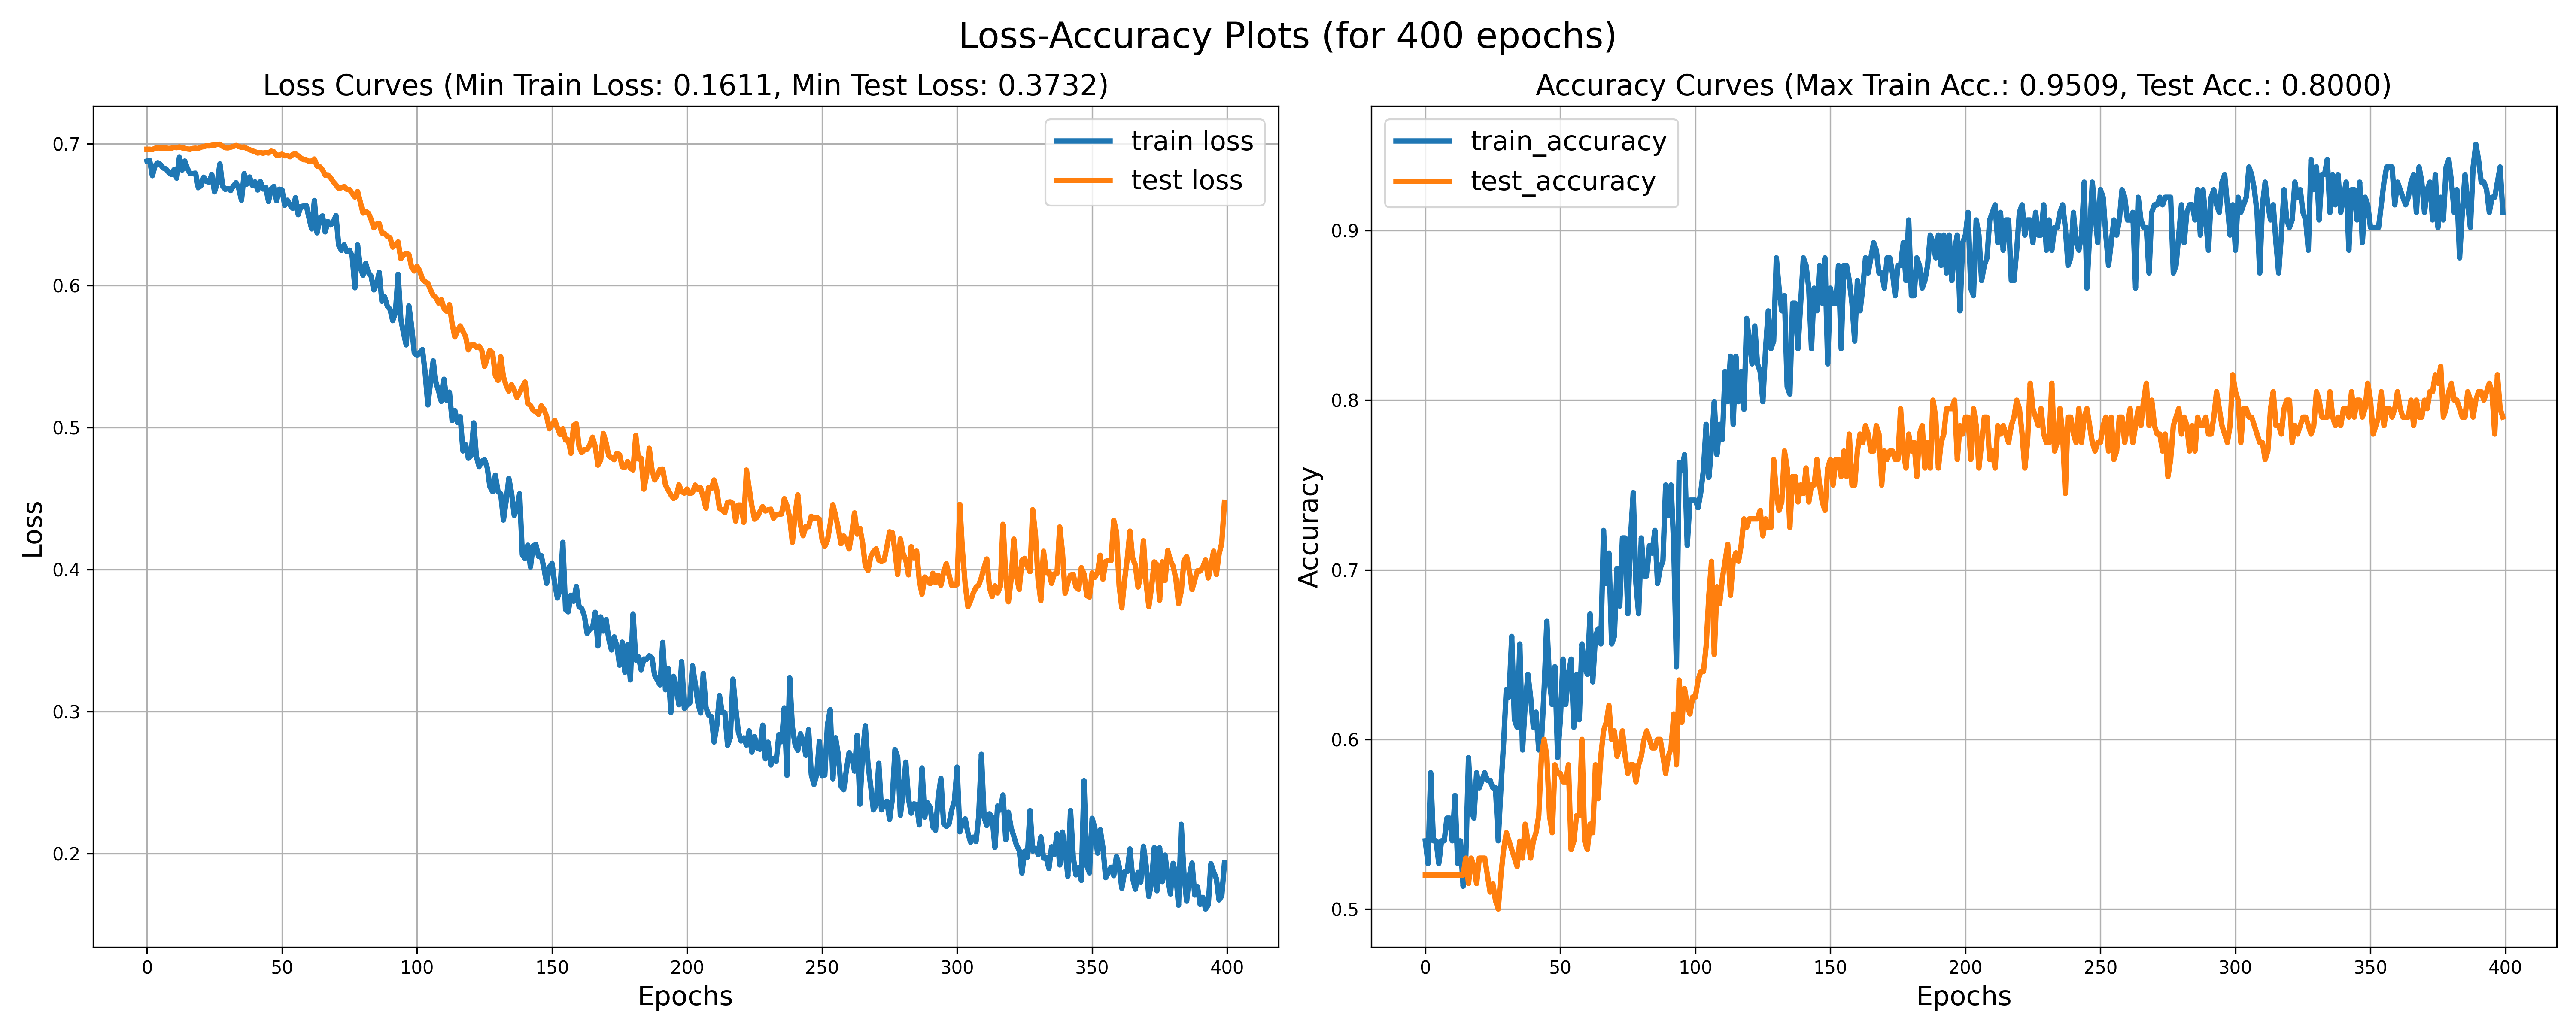
\includegraphics[width=0.9\textwidth]{plots/sinusoid_adam-lr-1e-3_more_layersloss_acc.png}
    \caption{Loss and accuracy for Circle dataset (train, test set with 200 points each)\\ Adam optimizer (lr $=1e-3$ ), 400 epochs, Cost function: CrossEntropyLoss, Xaiver initialization}
    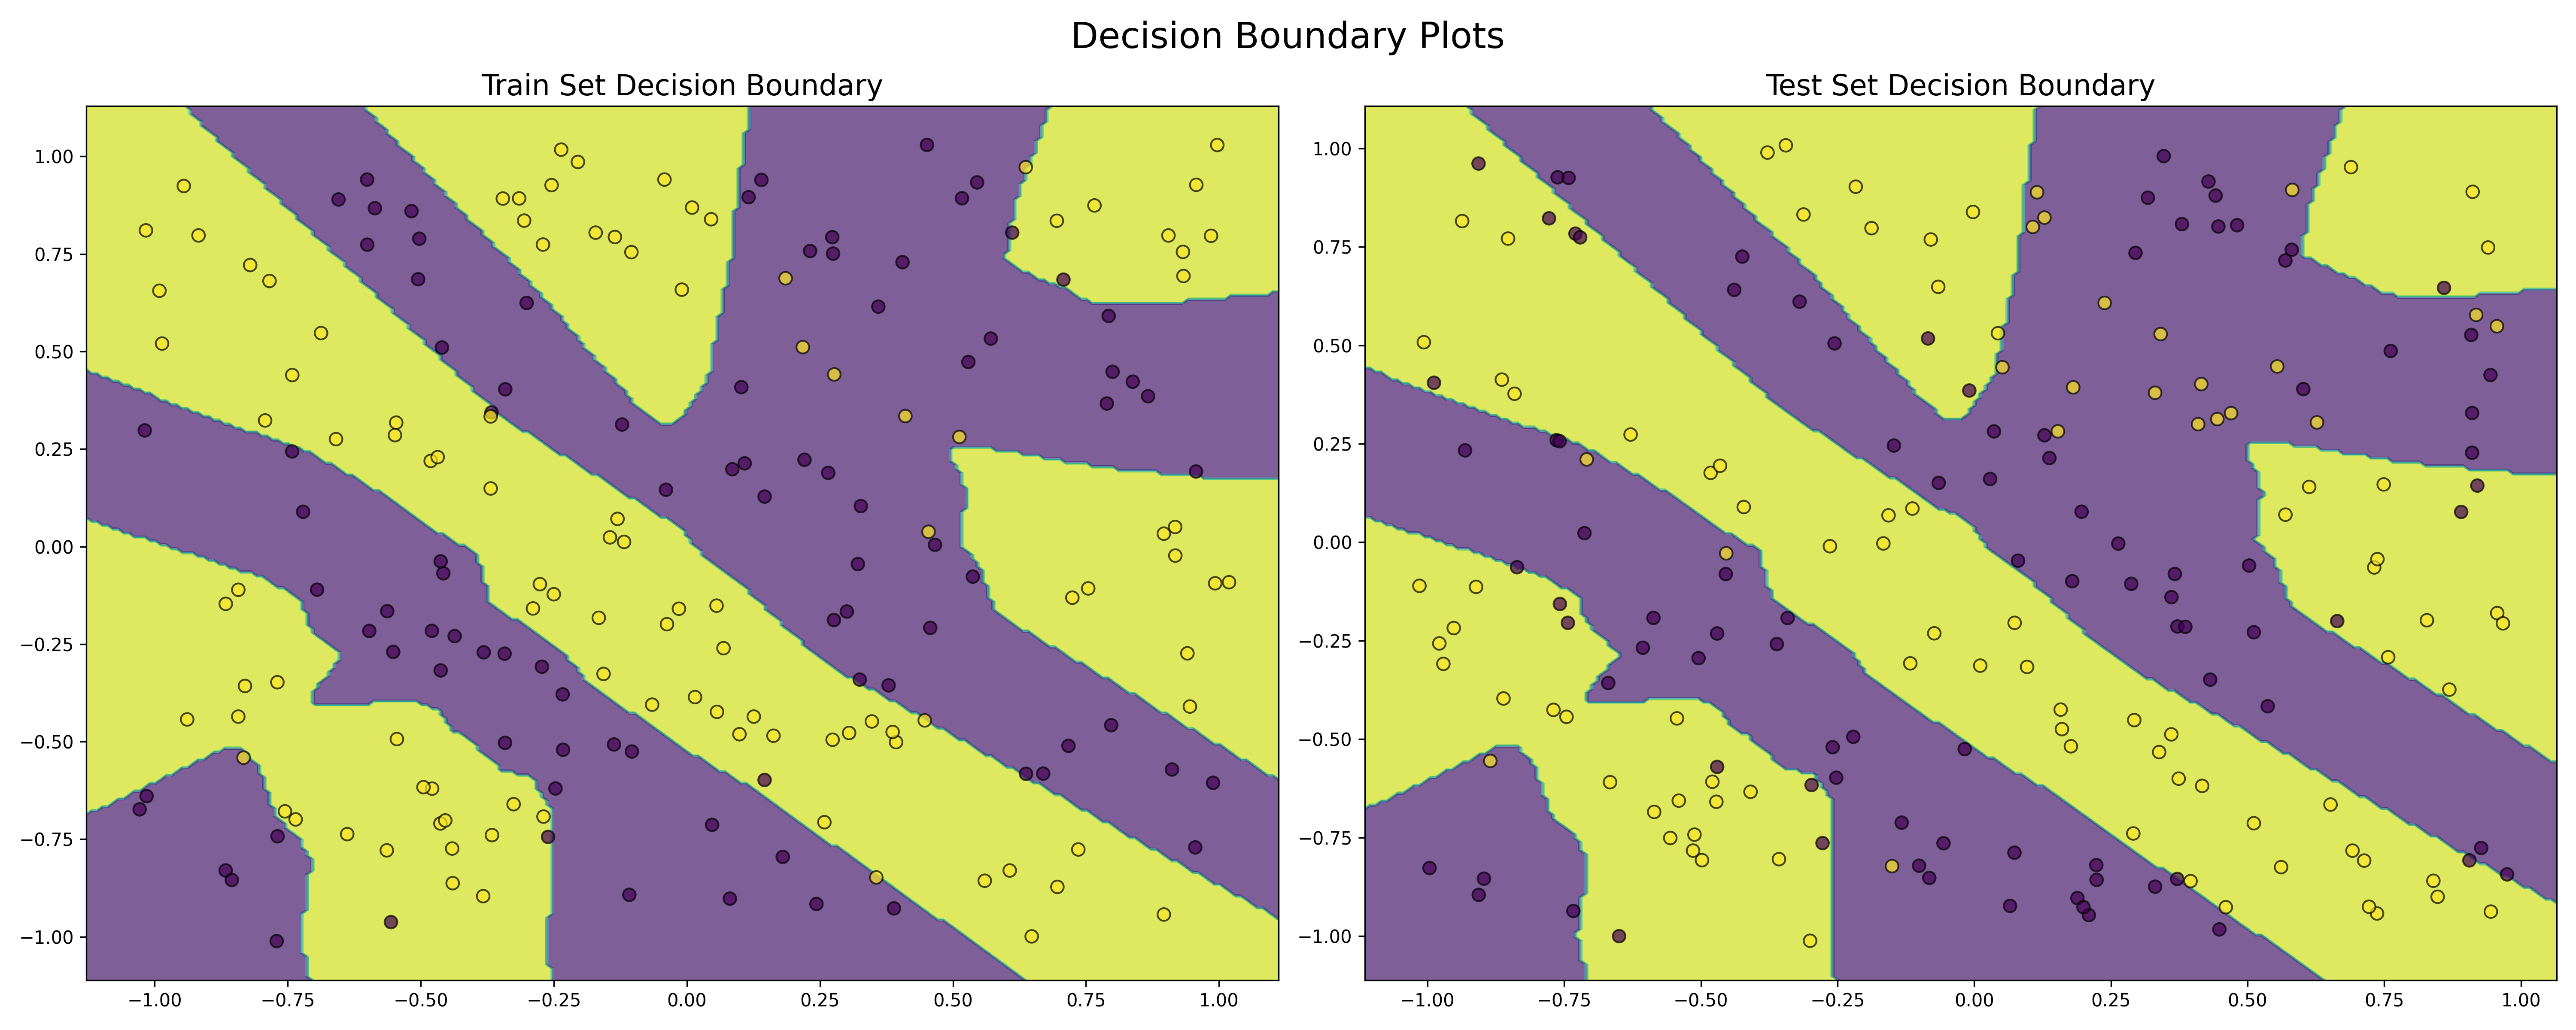
\includegraphics[width=0.8\textwidth]{plots/sinusoid_adam-lr-1e-3_more_layersboundary.png}
    \caption{(L2Loss) Decision boundary for Circle separable dataset (train, test set with 200 points each) 
    Adam optimizer (lr $=1e-3$)}
\end{figure}





\subsection{MLP with Adam Optimizer of learning rate 0.001 and default parameters}

\begin{figure}[H]
    \centering
    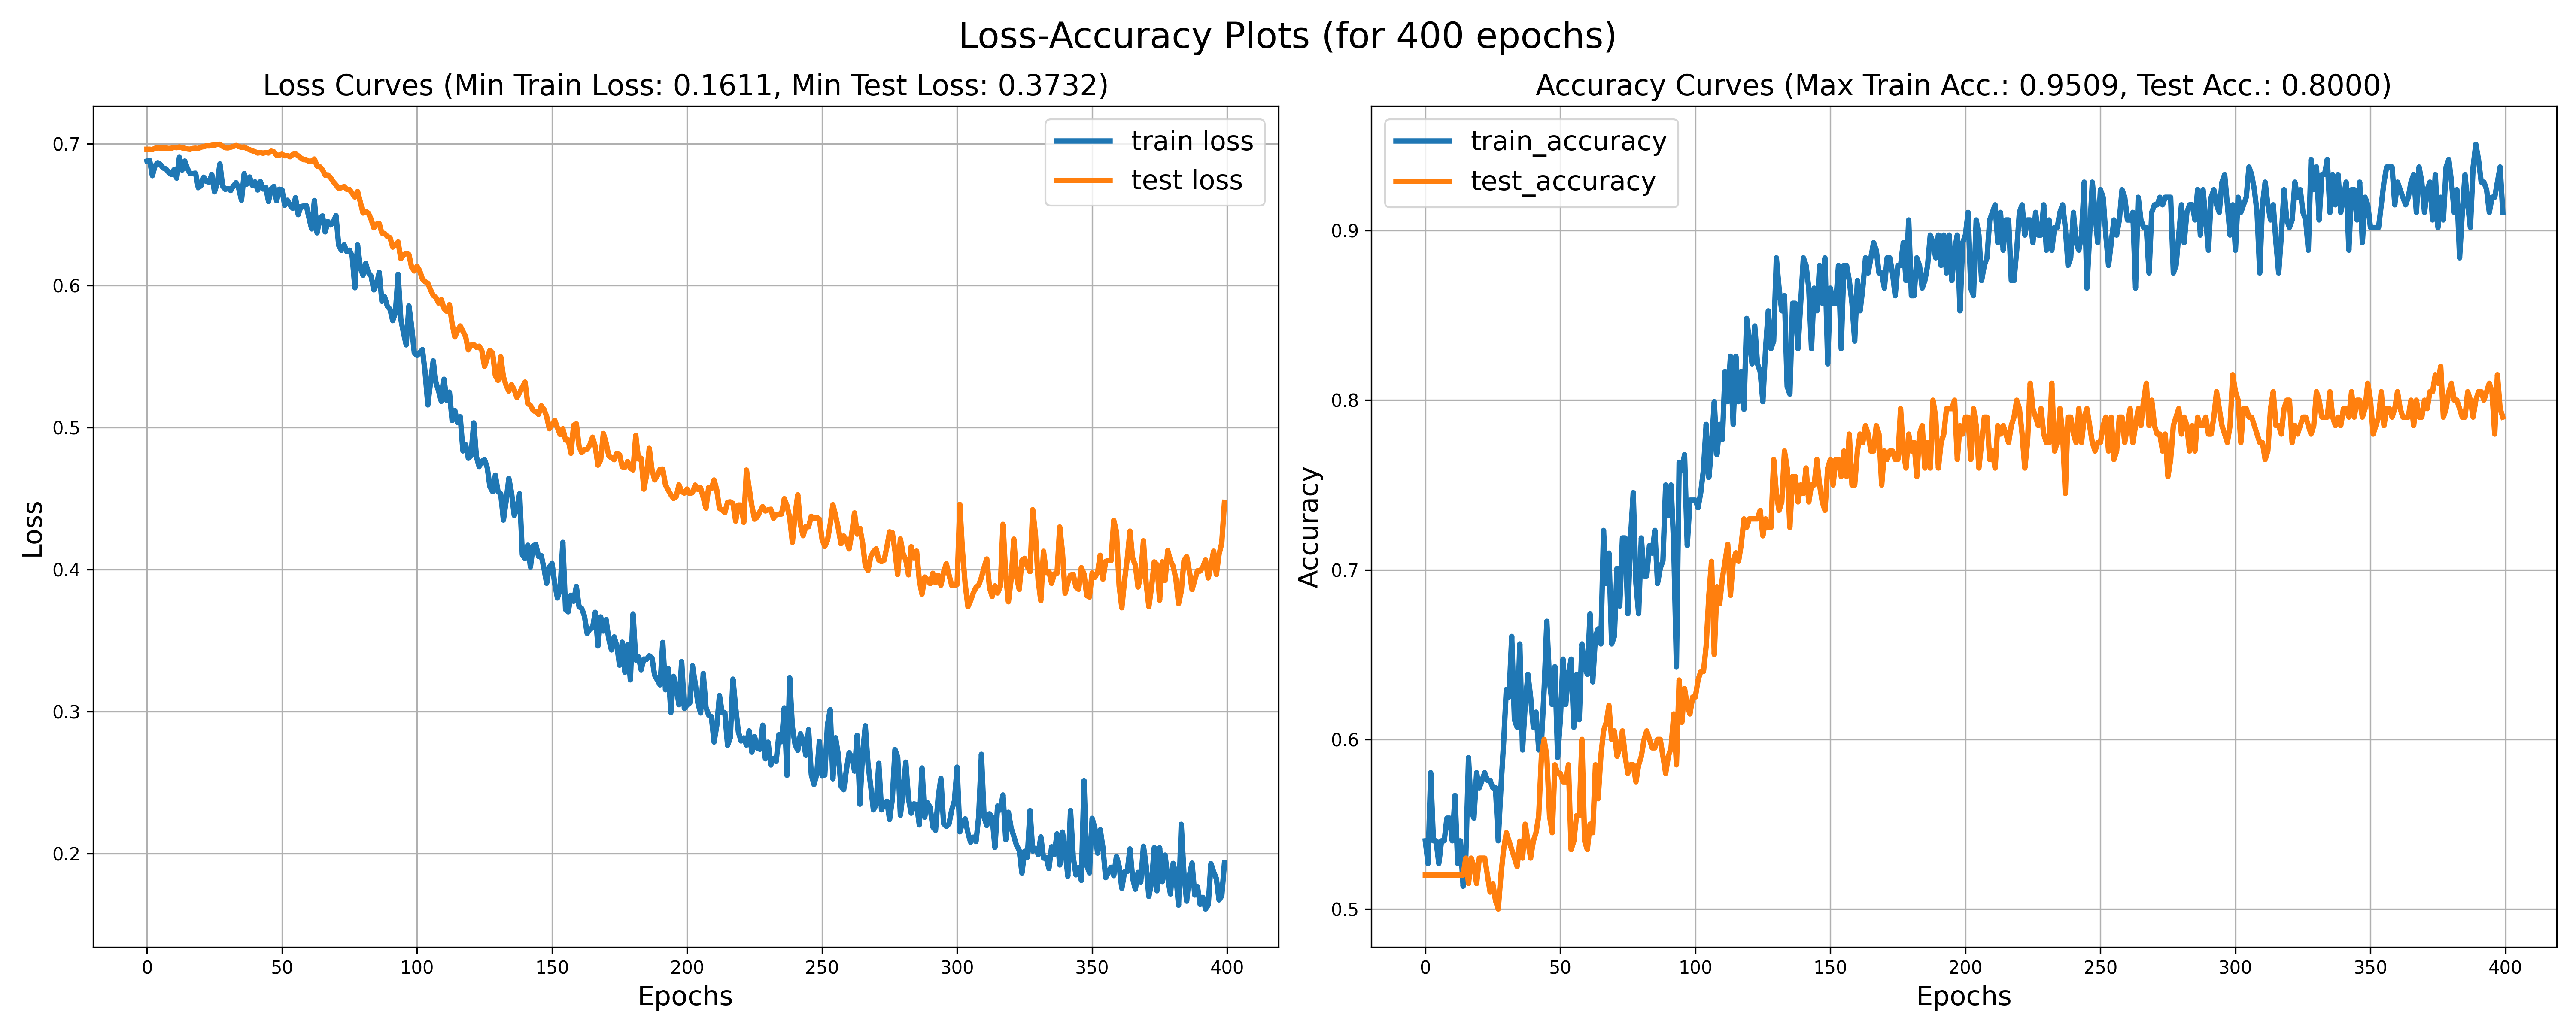
\includegraphics[width=0.9\textwidth]{plots/sinusoid_adam-lr-1e-3_more_layersloss_acc.png}
    \caption{Loss and accuracy for Circle dataset (train, test set with 200 points each)\\ Adam optimizer (lr $=1e-3$ ), 400 epochs, Cost function: CrossEntropyLoss, Xaiver initialization}
    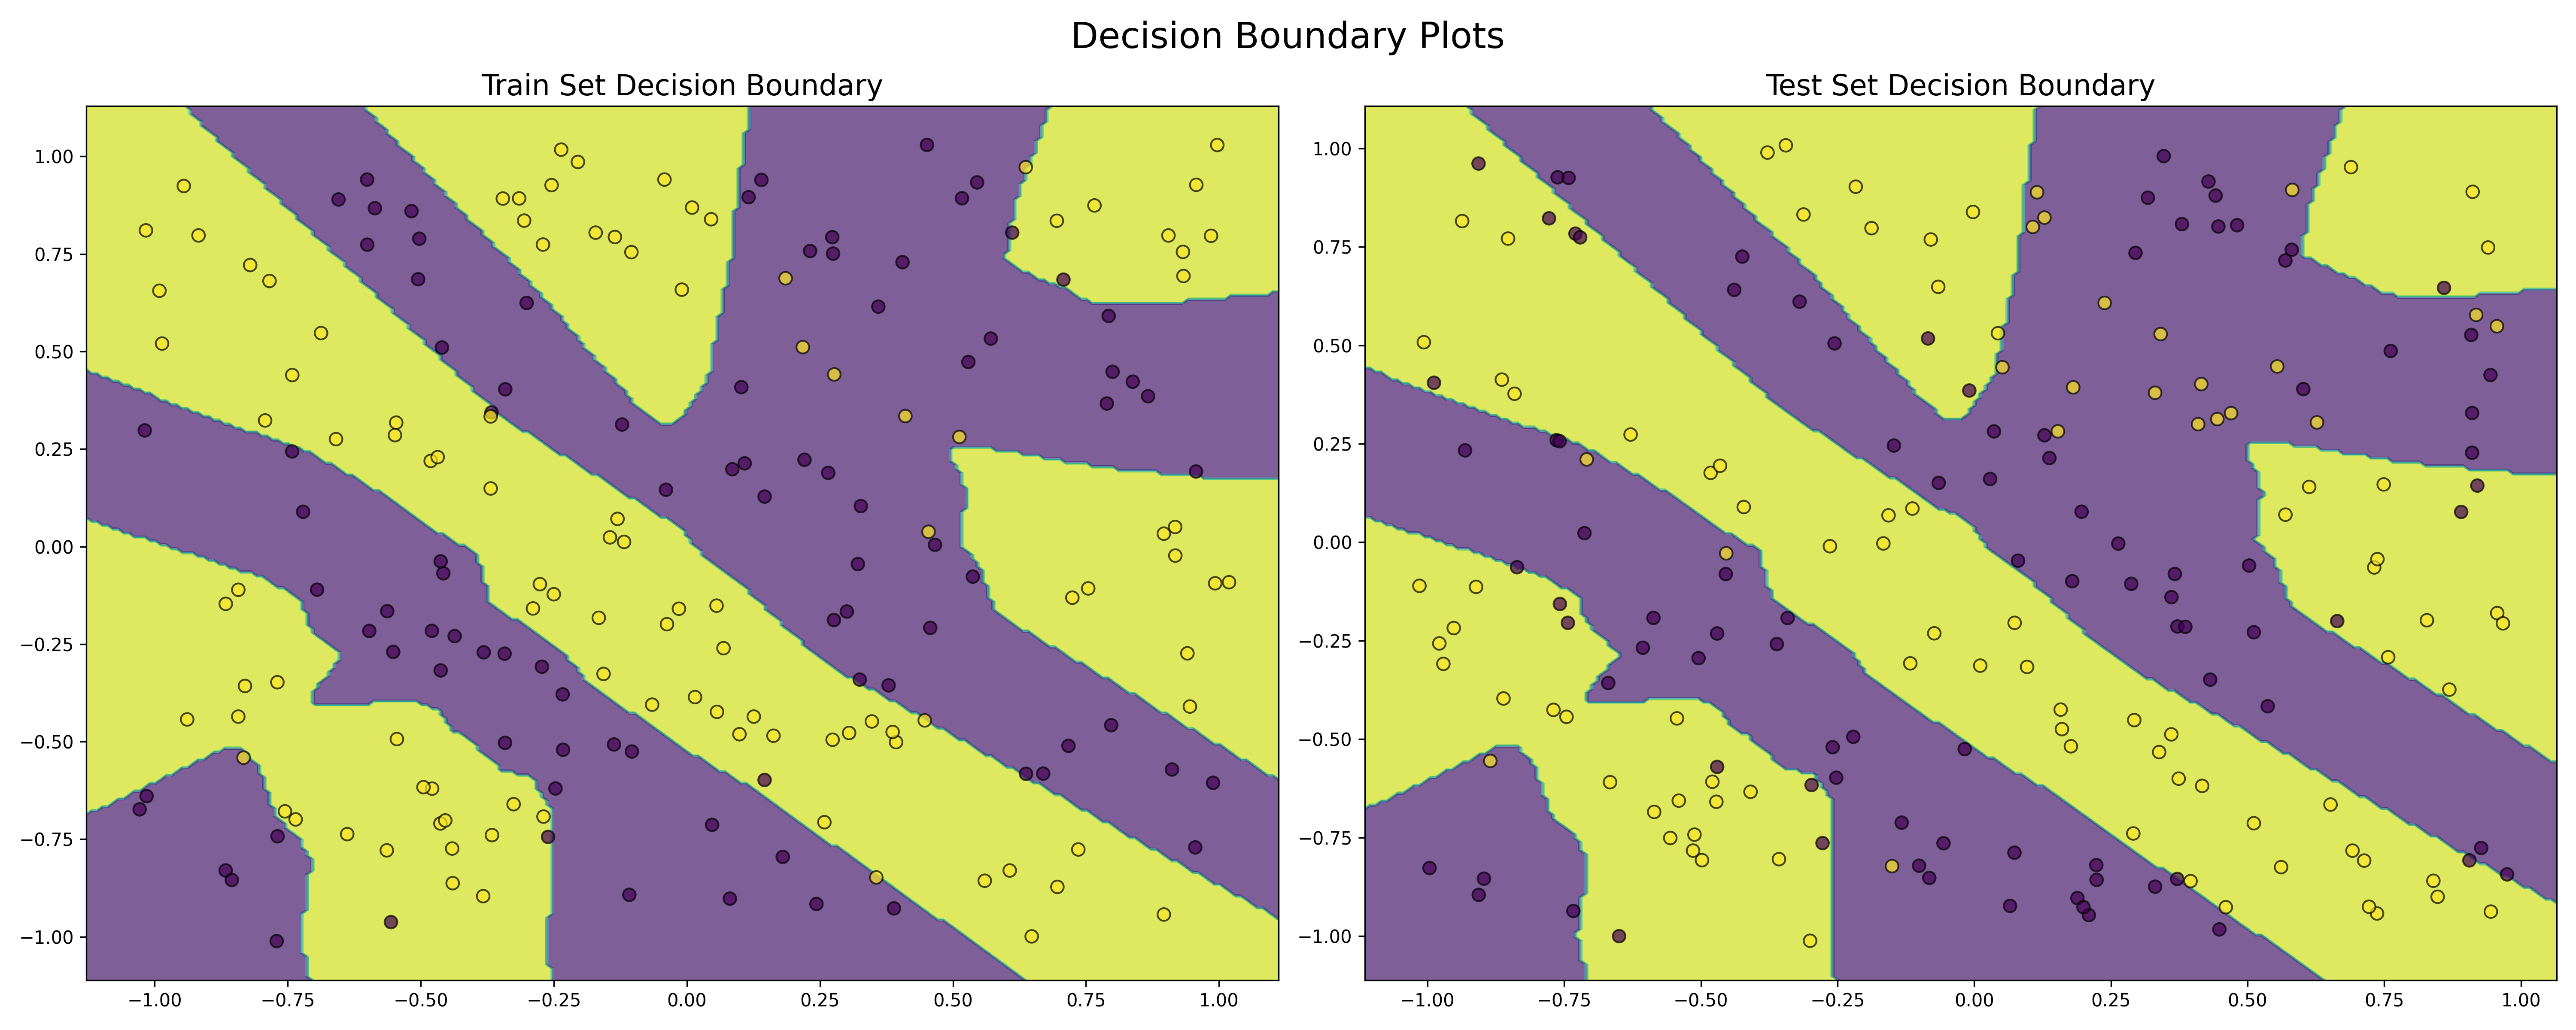
\includegraphics[width=0.8\textwidth]{plots/sinusoid_adam-lr-1e-3_more_layersboundary.png}
    \caption{(L2Loss) Decision boundary for Circle separable dataset (train, test set with 200 points each) 
    Adam optimizer (lr $=1e-3$)}
\end{figure}


% ############################################


\end{solve}

%%%%%%%%%%%%%%%%%%%%%%%%%%%%%%%%%%%%%%%%%%%%
\newpage

\section{Deliverable 6: Evasion attacks}

\textcolor{red}{\textbf{For all of the attacks, I have attached the ipynb notebook that has all the runs for the TAs to see}. The file is called attacks.ipynb}

\subsection{Task 1 (Untargeted) vs Task 2 (Targeted)}


\begin{solve}

I am only showing this for one image here, but tried for a set of three images and the results were similar.

The plots of purturbed images and the original images are shown below for both the tasks. The success rate and accuracy plots are also shown for both the models.

Note that the success rate for Untargeted attacks just means that there was misclassificaiton, whereeas for Targeted attacks, it means that the attack was successful in making the model predict the target class (in our case our class that we want to attack was 1 and we wanted the model to predict 8). 

We see that for epsilon .02 and .05 it is hard to see the difference between the original and the purturbed images, but for epsilon .1, the difference is visible. We start seeing artificats.

Note that in the case of targeted attacks, we used PGD. Given the value of $\alpha = .0392$, we see that the attack is quite visible even for $\epsilon \sim .04$


\textbf{Model A vs Model B for Targeted and Untargeted Attacks}
\begin{itemize}
    \item For Untargeted attacks, the success rate is higher for Model B than Model A, it remains constant for Model B, but changes for Model A.
    \item For Targeted attacks, the success rate is higher for Model A than Model B. Infact we are unable to get any successful attack on Model B even with very high $\epsilon$ values as compared to Model A for the same $\alpha$ values.
    We also see that the test accuracy does not change for model B dyring the attack, showing that not only we are failing in targeted attacks but we are also not able to misclassify the images in untargeted sense.
    This shows that Model B is more robust to targeted attacks than Model A in this setting.
    \item It might be that Model B is specifically trained to be robust to such targeted attacks, or it might be that Model B is more robust to such attacks in general. We cannot say this until we do tets on other kinds of targeted attacks and not just on $1$ and $8$ clases.
\end{itemize}


\subsubsection{Untargeted Attack}

\begin{figure}[H]
    \centering
    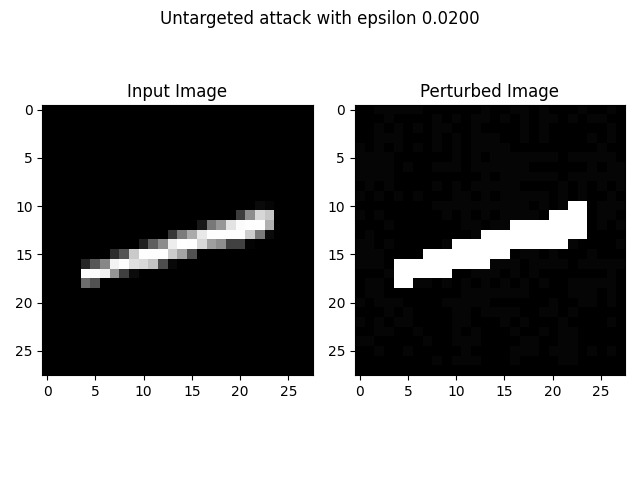
\includegraphics[trim={0 1.5cm 0cm 0}, width=.5\textwidth]{/Users/vashisth/Documents/GitHub/Intro_DL/IDL_HW3/HW3_tex/plots/Del6/Untargeted/Untargeted_attack__modA_0.0200_Img-2.png}
% \end{figure}
% \begin{figure}[H]
    \centering
    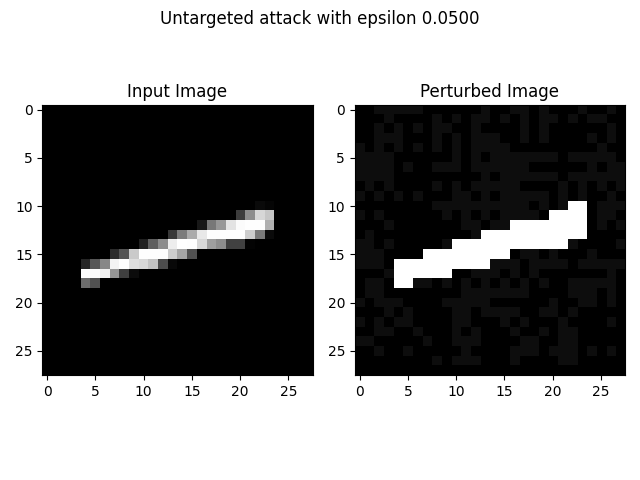
\includegraphics[trim={0 1.5cm 0cm 0}, width=.5\textwidth]{/Users/vashisth/Documents/GitHub/Intro_DL/IDL_HW3/HW3_tex/plots/Del6/Untargeted/Untargeted_attack__modA_0.0500_Img-2.png}
% \end{figure}

% \begin{figure}[H]
    \centering
    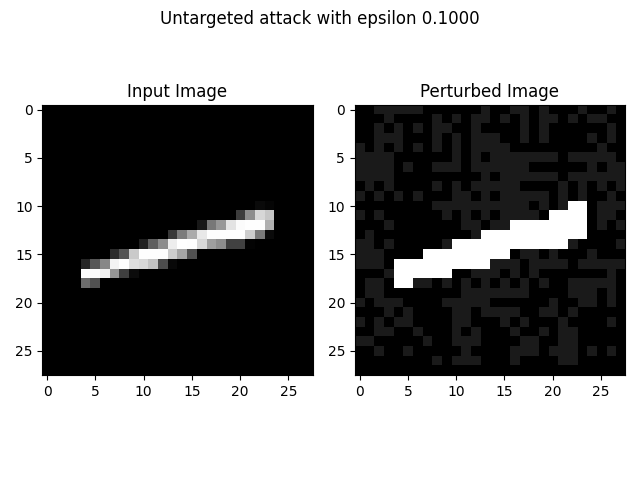
\includegraphics[trim={0 1.5cm 0cm 0}, width=.5\textwidth]{/Users/vashisth/Documents/GitHub/Intro_DL/IDL_HW3/HW3_tex/plots/Del6/Untargeted/Untargeted_attack__modA_0.1000_Img-2.png}
    \caption{Untargeted Attack on Model A for Image with index 2 for different $\epsilon$}
\end{figure}
% [width = .99\textwidth]


\begin{figure}[H]
    \centering
    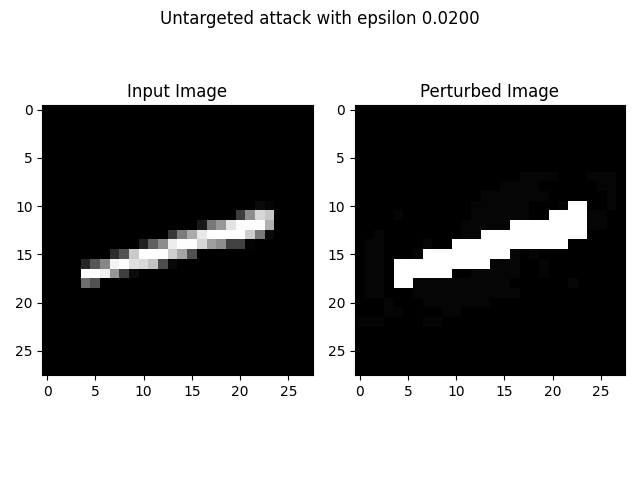
\includegraphics[trim={0 1.5cm 0cm 0}, width=.5\textwidth]{/Users/vashisth/Documents/GitHub/Intro_DL/IDL_HW3/HW3_tex/plots/Del6/Untargeted/Untargeted_attack__modB_0.0200_Img-2.png}
% \end{figure}
% \begin{figure}[H]
    \centering
    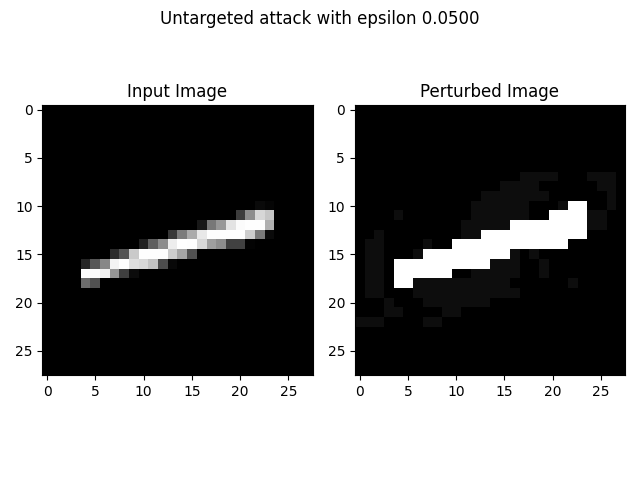
\includegraphics[trim={0 1.5cm 0cm 0}, width=.5\textwidth]{/Users/vashisth/Documents/GitHub/Intro_DL/IDL_HW3/HW3_tex/plots/Del6/Untargeted/Untargeted_attack__modB_0.0500_Img-2.png}
% \end{figure}

% \begin{figure}[H]
    \centering
    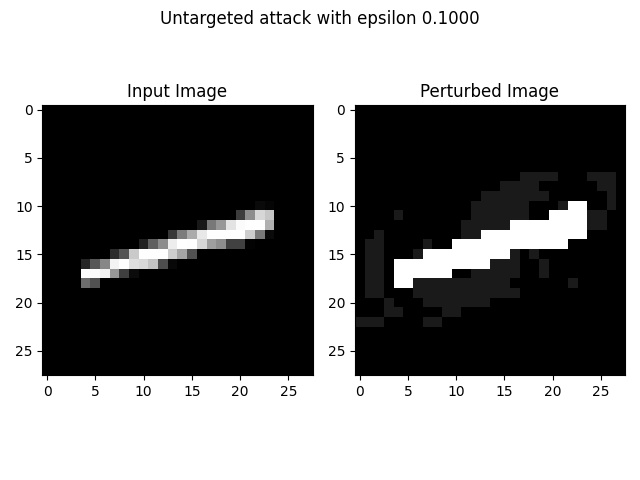
\includegraphics[trim={0 1.5cm 0cm 0}, width=.5\textwidth]{/Users/vashisth/Documents/GitHub/Intro_DL/IDL_HW3/HW3_tex/plots/Del6/Untargeted/Untargeted_attack__modB_0.1000_Img-2.png}
    \caption{Untargeted Attack on Model B for Image with index 2 for different $\epsilon$}
\end{figure}

\begin{figure}[H]
\centering
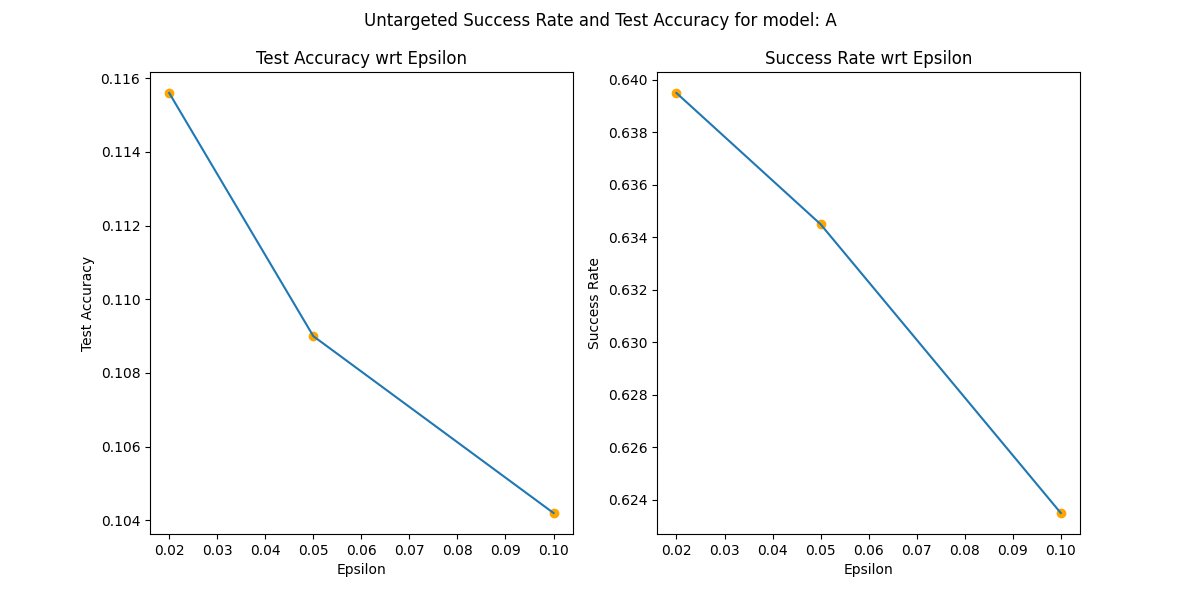
\includegraphics[width = .6 \textwidth]{/Users/vashisth/Documents/GitHub/Intro_DL/IDL_HW3/HW3_tex/plots/Del6/success_rate_plot_Untargeted_modA.png}
\caption{Success Rate and Accuracy Plot for Untargeted Attack on Model A}
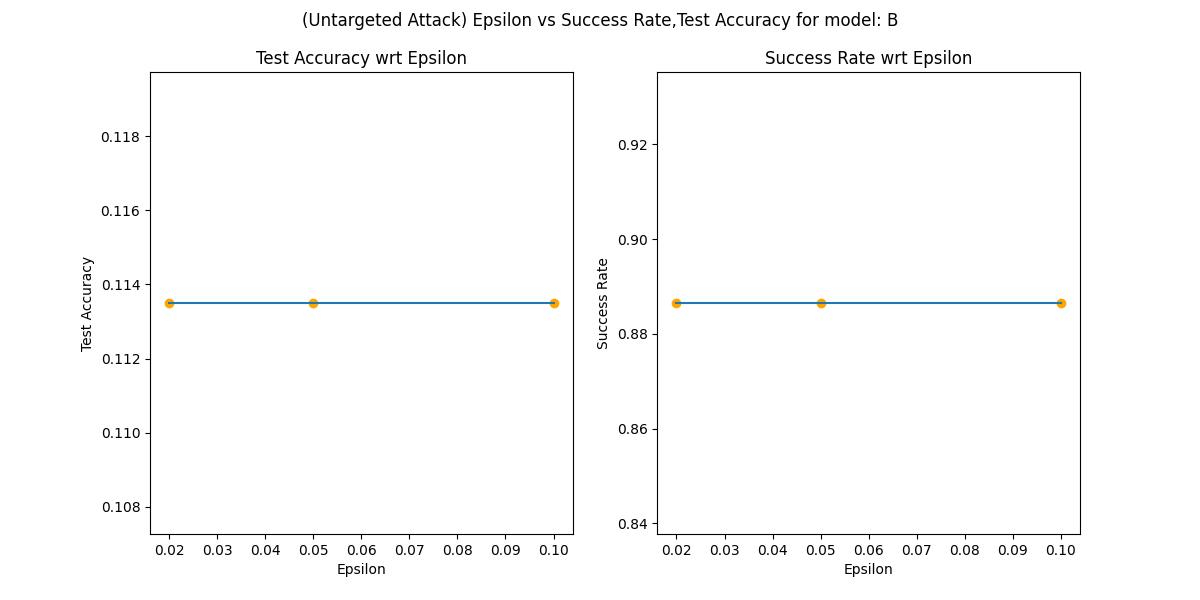
\includegraphics[width = .6 \textwidth]{/Users/vashisth/Documents/GitHub/Intro_DL/IDL_HW3/HW3_tex/plots/Del6/success_rate_plot_(Untargeted Attack)_modB.png}
\caption{Success Rate and Accuracy Plot for Untargeted Attack on Model B}
\end{figure}

% \end{solve}


%%%%%%%%%%%%%%%%%%%%%%%%%%%%%%%%%%%%%%%%%%

\subsubsection{Targeted Attack}

% \begin{solve}
\begin{figure}[H]
    \centering
    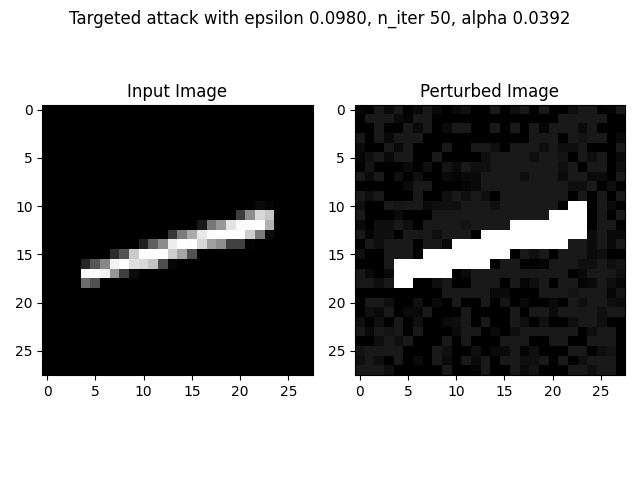
\includegraphics[trim={0 1.5cm 0cm 0}, width=.5\textwidth]{/Users/vashisth/Documents/GitHub/Intro_DL/IDL_HW3/HW3_tex/plots/Del6/Targeted/Targeted_attack__modA_e-0.0980_a-0.0392Img-2_iter50.png}
% \end{figure}
    \centering
    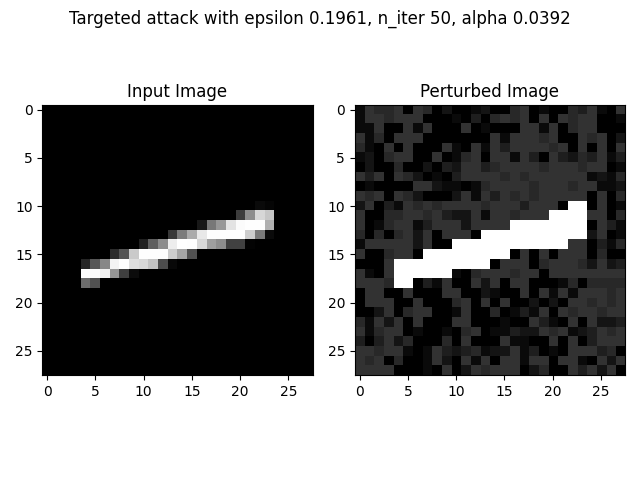
\includegraphics[trim={0 1.5cm 0cm 0}, width=.5\textwidth]{/Users/vashisth/Documents/GitHub/Intro_DL/IDL_HW3/HW3_tex/plots/Del6/Targeted/Targeted_attack__modA_e-0.1961_a-0.0392Img-2_iter50.png}
% \end{figure}
    \centering
    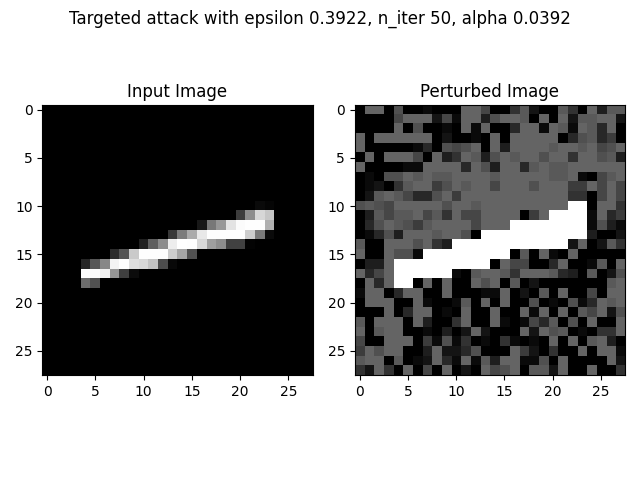
\includegraphics[trim={0 1.5cm 0cm 0}, width=.5\textwidth]{/Users/vashisth/Documents/GitHub/Intro_DL/IDL_HW3/HW3_tex/plots/Del6/Targeted/Targeted_attack__modA_e-0.3922_a-0.0392Img-2_iter50.png}
    \caption{Targeted Attack on Model A for Image with index 2 for different $\epsilon$}
\end{figure}



\begin{figure}[H]
    \centering
    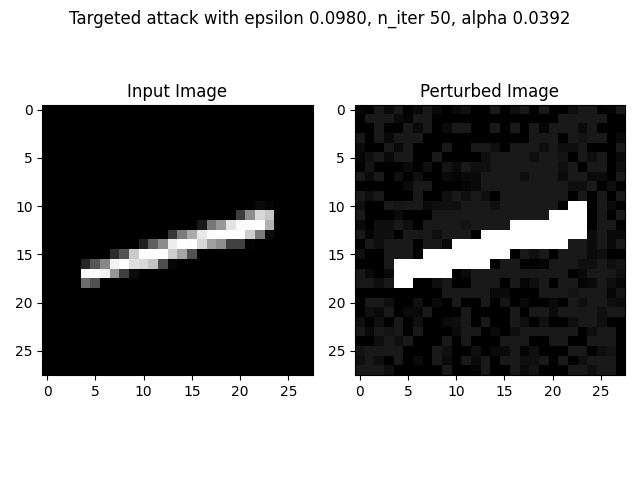
\includegraphics[trim={0 1.5cm 0cm 0}, width=.4\textwidth]{/Users/vashisth/Documents/GitHub/Intro_DL/IDL_HW3/HW3_tex/plots/Del6/Targeted/Targeted_attack__modA_e-0.0980_a-0.0392Img-2_iter50.png}
% \end{figure}
    \centering
    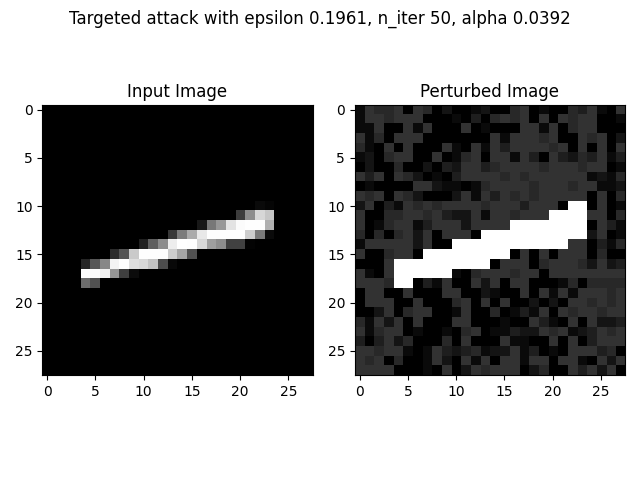
\includegraphics[trim={0 1.5cm 0cm 0}, width=.4\textwidth]{/Users/vashisth/Documents/GitHub/Intro_DL/IDL_HW3/HW3_tex/plots/Del6/Targeted/Targeted_attack__modA_e-0.1961_a-0.0392Img-2_iter50.png}
% \end{figure}
    \centering
    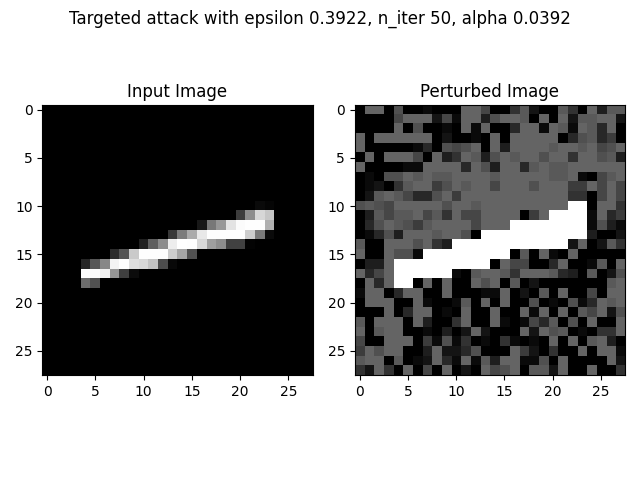
\includegraphics[trim={0 1.5cm 0cm 0}, width=.4\textwidth]{/Users/vashisth/Documents/GitHub/Intro_DL/IDL_HW3/HW3_tex/plots/Del6/Targeted/Targeted_attack__modA_e-0.3922_a-0.0392Img-2_iter50.png}
    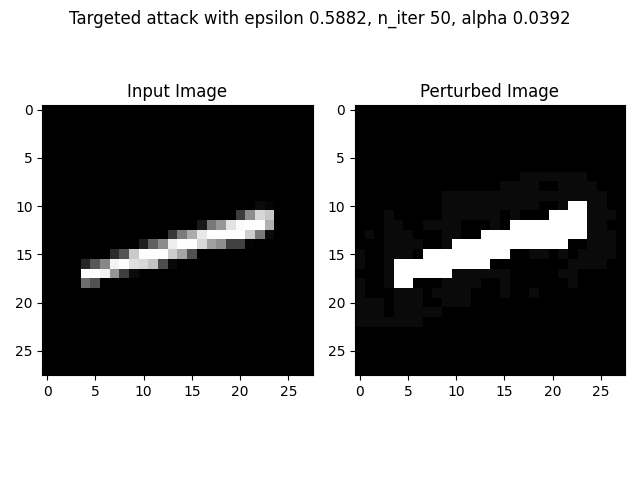
\includegraphics[trim = {0 1.5cm 0 0}, width = .4\textwidth] {/Users/vashisth/Documents/GitHub/Intro_DL/IDL_HW3/HW3_tex/plots/Del6/Targeted/Targeted_attack__modB_e-0.5882_a-0.0392Img-2_iter50.png}
    %%%%%
    \caption{Targeted Attack on Model B for Image with index 2 for different $\epsilon$ and $\alpha$ = 0.0392}
\end{figure}


\begin{figure}[H]
\centering
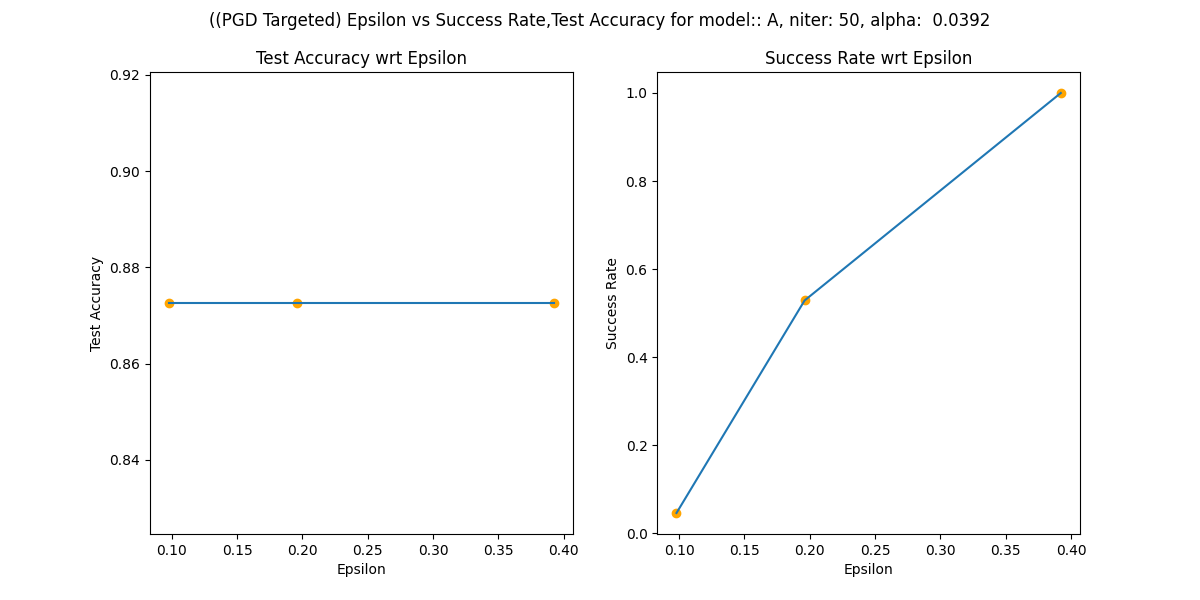
\includegraphics[width = .6 \textwidth]{/Users/vashisth/Documents/GitHub/Intro_DL/IDL_HW3/HW3_tex/plots/Del6/success_rate_plot_(PGD Targeted)_modA_iter50_a-0.0392.png}
\caption{Success Rate and Accuracy Plot for Targeted Attack on Model A}
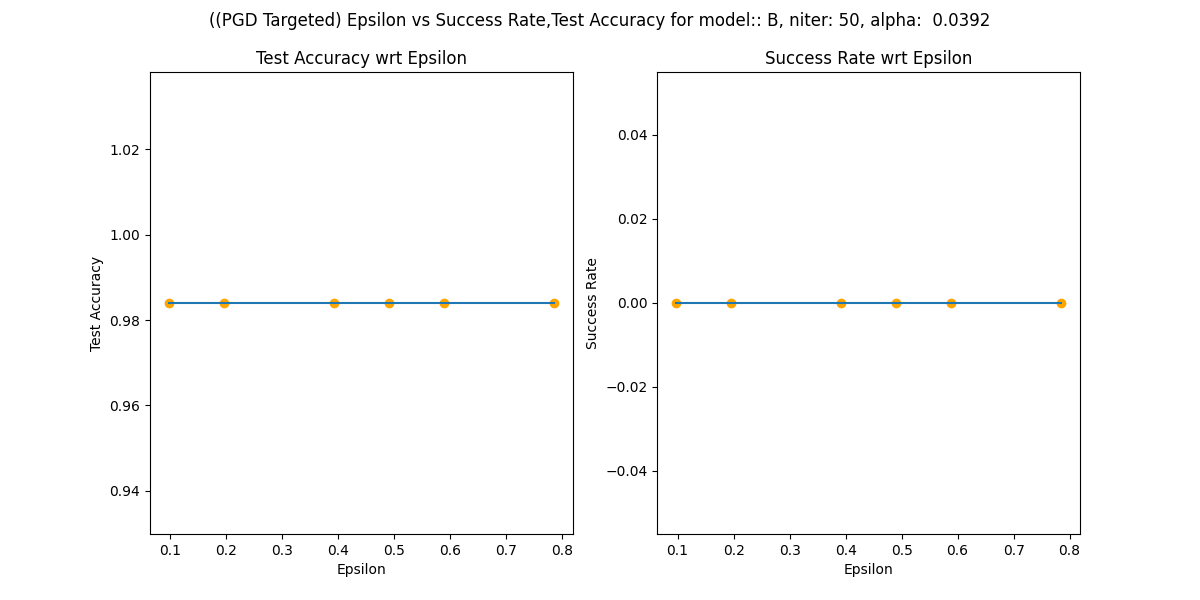
\includegraphics[width = .6 \textwidth]{/Users/vashisth/Documents/GitHub/Intro_DL/IDL_HW3/HW3_tex/plots/Del6/success_rate_plot_(PGD Targeted)_modB_iter50_a-0.0392.png}
\caption{Success Rate and Accuracy Plot for Targeted Attack on Model B}
\end{figure}

\end{solve}
%%%%%%%%%%%%%%%%%%%%%%%%%%%%%%%%%%%%%%%%%%%%%%%%%%%

% \subsubsection{Task 1 (Untargeted) vs Task 2 (Targeted)}


% \begin{solve}

% I am only showing this for one image here, but tried for a set of three images and the results were similar.

% The plots of purturbed images and the original images are shown below for both the tasks. The success rate and accuracy plots are also shown for both the models.

% Note that the success rate for Untargeted attacks just means that there was misclassificaiton, whereeas for Targeted attacks, it means that the attack was successful in making the model predict the target class (in our case our class that we want to attack was 1 and we wanted the model to predict 8). 

% We see that for epsilon .02 and .05 it is hard to see the difference between the original and the purturbed images, but for epsilon .1, the difference is visible. We start seeing artificats.

% Note that in the case of targeted attacks, we used PGD. Given the value of $\alpha = .0392$, we see that the attack is quite visible even for $\epsilon \sim .04$


% \textbf{Model A vs Model B}
% \begin{itemize}
%     \item For Untargeted attacks, the success rate is higher for Model B than Model A, it remains constant for Model B, but changes for Model A.
%     \item For Targeted attacks, the success rate is higher for Model A than Model B. This is because Model A is more accurate than Model B.
% \end{itemize}


% \subsubsection{Untargeted Attack}

% \begin{figure}[H]
%     \centering
%     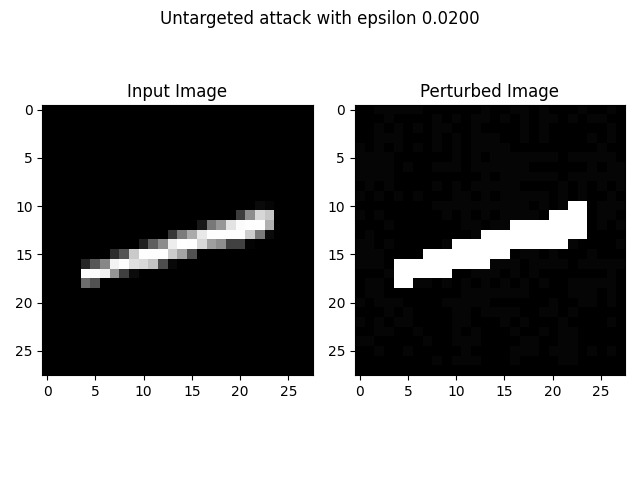
\includegraphics[trim={0 1.5cm 0cm 0}, width=.5\textwidth]{/Users/vashisth/Documents/GitHub/Intro_DL/IDL_HW3/HW3_tex/plots/Del6/Untargeted/Untargeted_attack__modA_0.0200_Img-2.png}
% % \end{figure}
% % \begin{figure}[H]
%     \centering
%     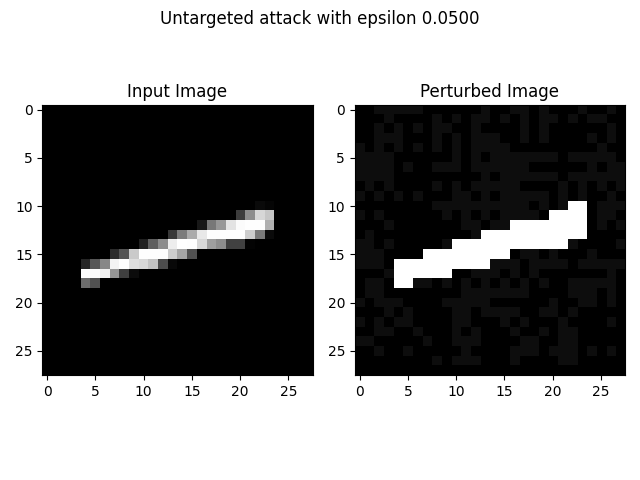
\includegraphics[trim={0 1.5cm 0cm 0}, width=.5\textwidth]{/Users/vashisth/Documents/GitHub/Intro_DL/IDL_HW3/HW3_tex/plots/Del6/Untargeted/Untargeted_attack__modA_0.0500_Img-2.png}
% % \end{figure}

% % \begin{figure}[H]
%     \centering
%     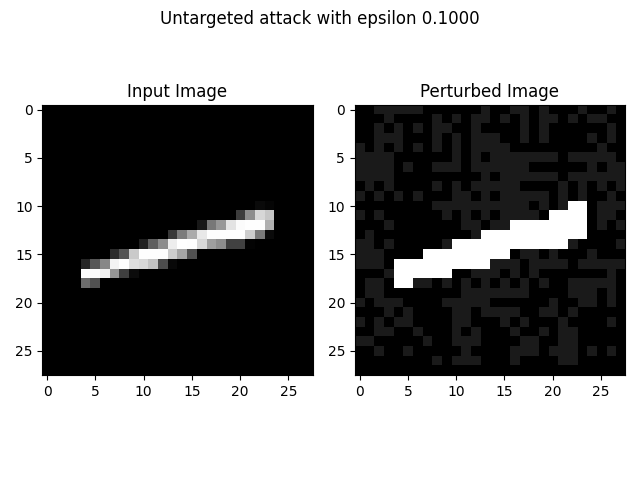
\includegraphics[trim={0 1.5cm 0cm 0}, width=.5\textwidth]{/Users/vashisth/Documents/GitHub/Intro_DL/IDL_HW3/HW3_tex/plots/Del6/Untargeted/Untargeted_attack__modA_0.1000_Img-2.png}
%     \caption{Untargeted Attack on Model A for Image with index 2 for different $\epsilon$}
% \end{figure}
% % [width = .99\textwidth]


% \begin{figure}[H]
%     \centering
%     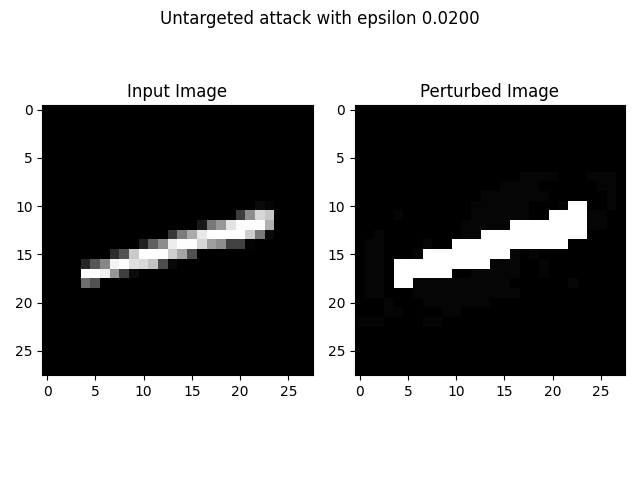
\includegraphics[trim={0 1.5cm 0cm 0}, width=.5\textwidth]{/Users/vashisth/Documents/GitHub/Intro_DL/IDL_HW3/HW3_tex/plots/Del6/Untargeted/Untargeted_attack__modB_0.0200_Img-2.png}
% % \end{figure}
% % \begin{figure}[H]
%     \centering
%     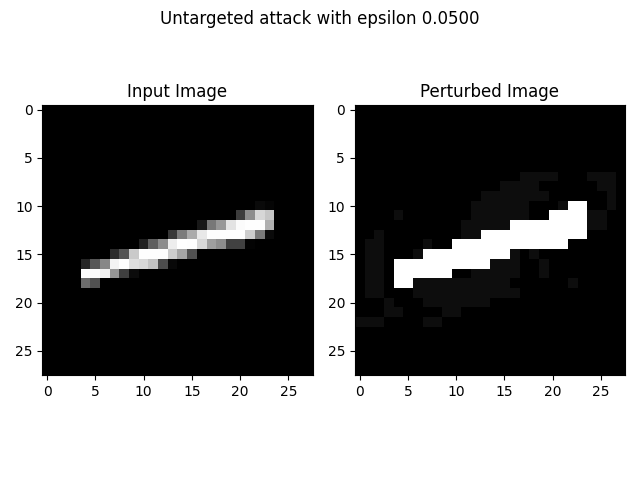
\includegraphics[trim={0 1.5cm 0cm 0}, width=.5\textwidth]{/Users/vashisth/Documents/GitHub/Intro_DL/IDL_HW3/HW3_tex/plots/Del6/Untargeted/Untargeted_attack__modB_0.0500_Img-2.png}
% % \end{figure}

% % \begin{figure}[H]
%     \centering
%     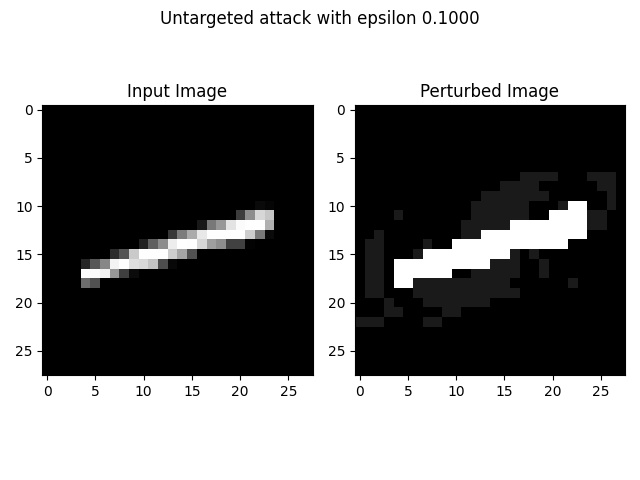
\includegraphics[trim={0 1.5cm 0cm 0}, width=.5\textwidth]{/Users/vashisth/Documents/GitHub/Intro_DL/IDL_HW3/HW3_tex/plots/Del6/Untargeted/Untargeted_attack__modB_0.1000_Img-2.png}
%     \caption{Untargeted Attack on Model B for Image with index 2 for different $\epsilon$}
% \end{figure}

% \begin{figure}[H]
% \centering
% 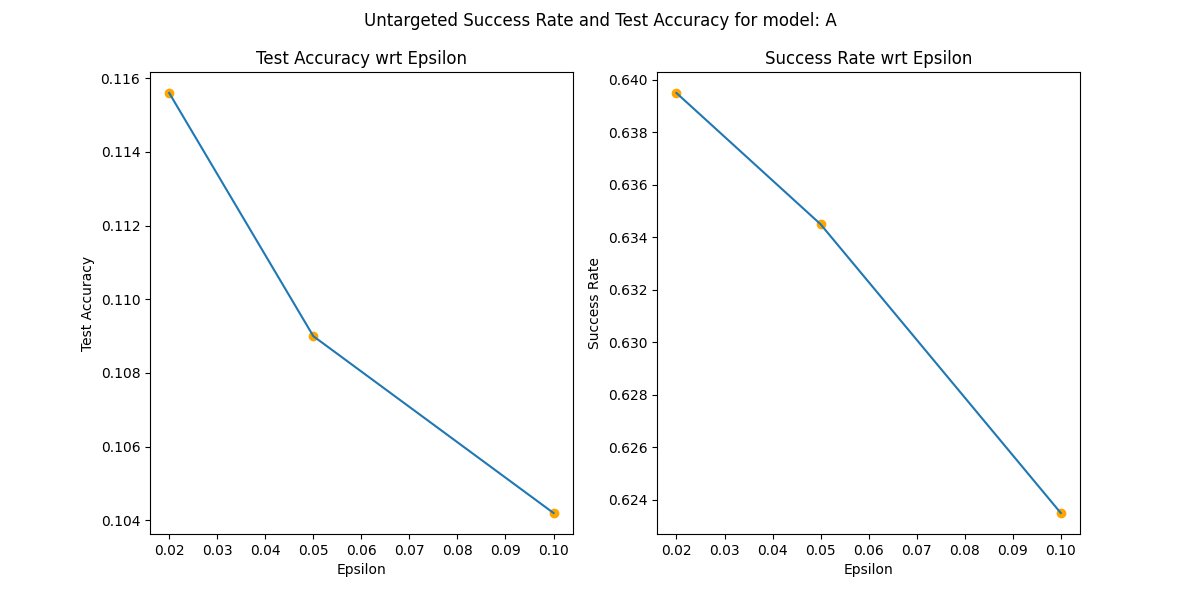
\includegraphics[width = .6 \textwidth]{/Users/vashisth/Documents/GitHub/Intro_DL/IDL_HW3/HW3_tex/plots/Del6/success_rate_plot_Untargeted_modA.png}
% \caption{Success Rate and Accuracy Plot for Untargeted Attack on Model A}
% 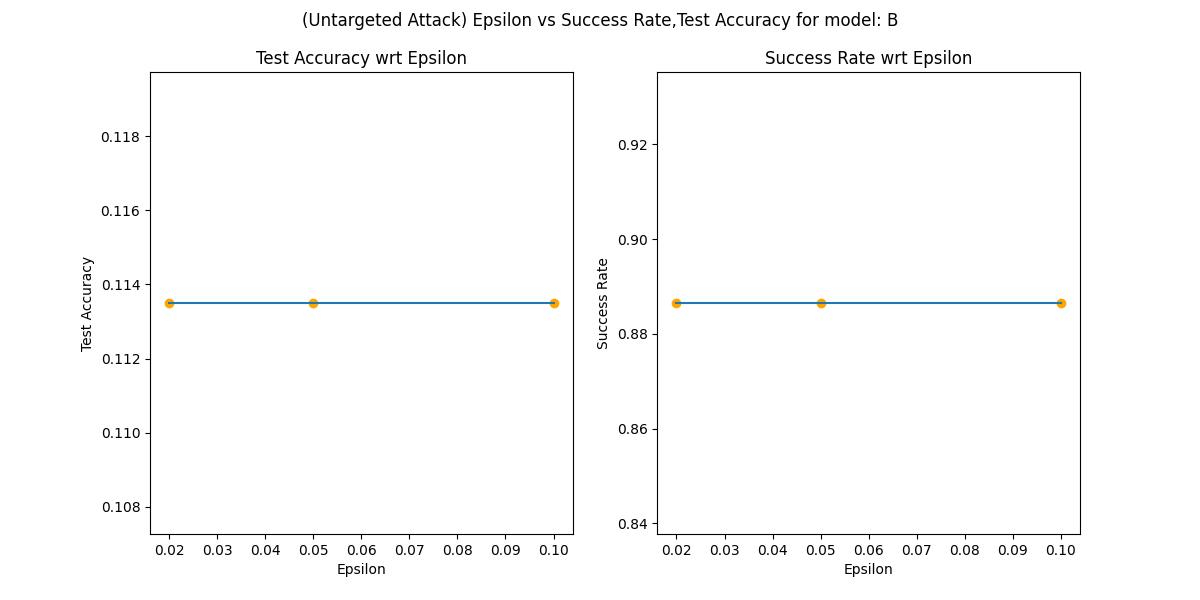
\includegraphics[width = .6 \textwidth]{/Users/vashisth/Documents/GitHub/Intro_DL/IDL_HW3/HW3_tex/plots/Del6/success_rate_plot_(Untargeted Attack)_modB.png}
% \caption{Success Rate and Accuracy Plot for Untargeted Attack on Model B}
% \end{figure}

% % \end{solve}


% %%%%%%%%%%%%%%%%%%%%%%%%%%%%%%%%%%%%%%%%%%

% \subsubsection{Targeted Attack}

% % \begin{solve}
% \begin{figure}[H]
%     \centering
%     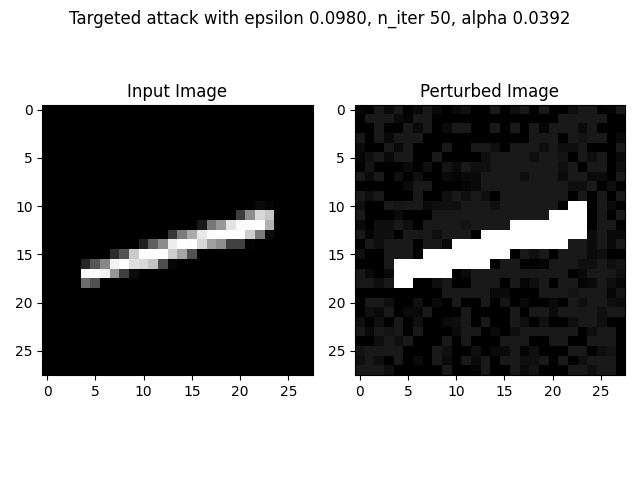
\includegraphics[trim={0 1.5cm 0cm 0}, width=.5\textwidth]{/Users/vashisth/Documents/GitHub/Intro_DL/IDL_HW3/HW3_tex/plots/Del6/Targeted/Targeted_attack__modA_e-0.0980_a-0.0392Img-2_iter50.png}
% % \end{figure}
%     \centering
%     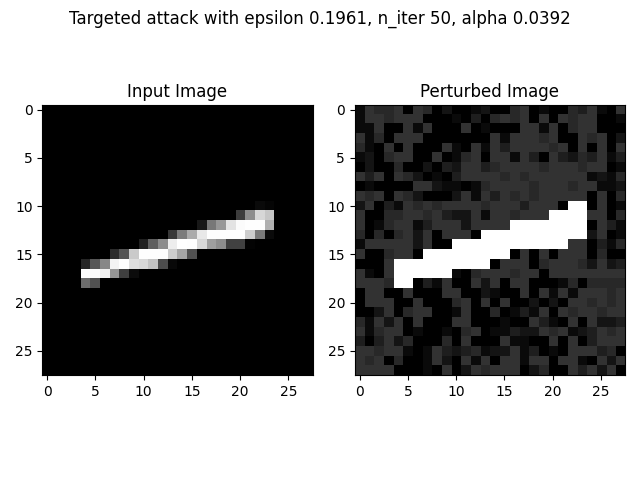
\includegraphics[trim={0 1.5cm 0cm 0}, width=.5\textwidth]{/Users/vashisth/Documents/GitHub/Intro_DL/IDL_HW3/HW3_tex/plots/Del6/Targeted/Targeted_attack__modA_e-0.1961_a-0.0392Img-2_iter50.png}
% % \end{figure}
%     \centering
%     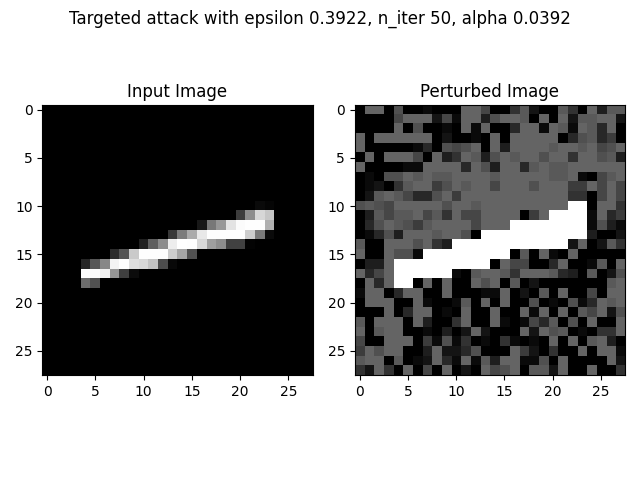
\includegraphics[trim={0 1.5cm 0cm 0}, width=.5\textwidth]{/Users/vashisth/Documents/GitHub/Intro_DL/IDL_HW3/HW3_tex/plots/Del6/Targeted/Targeted_attack__modA_e-0.3922_a-0.0392Img-2_iter50.png}
%     \caption{Targeted Attack on Model A for Image with index 2 for different $\epsilon$}
% \end{figure}



% \begin{figure}[H]
%     \centering
%     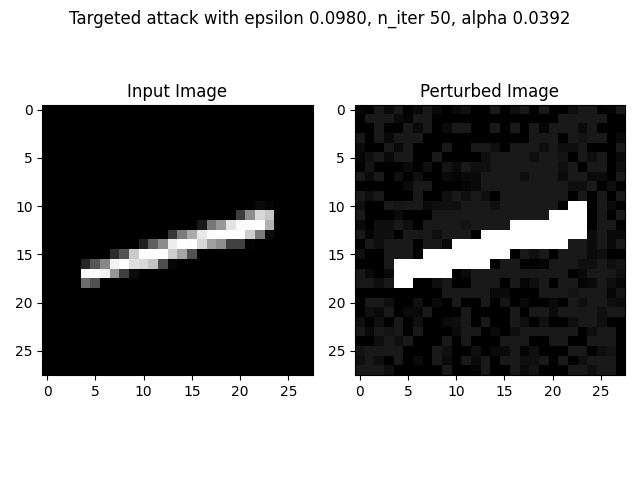
\includegraphics[trim={0 1.5cm 0cm 0}, width=.4\textwidth]{/Users/vashisth/Documents/GitHub/Intro_DL/IDL_HW3/HW3_tex/plots/Del6/Targeted/Targeted_attack__modA_e-0.0980_a-0.0392Img-2_iter50.png}
% % \end{figure}
%     \centering
%     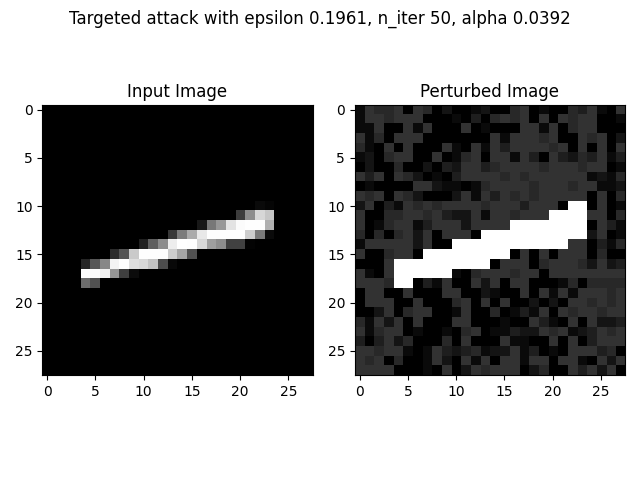
\includegraphics[trim={0 1.5cm 0cm 0}, width=.4\textwidth]{/Users/vashisth/Documents/GitHub/Intro_DL/IDL_HW3/HW3_tex/plots/Del6/Targeted/Targeted_attack__modA_e-0.1961_a-0.0392Img-2_iter50.png}
% % \end{figure}
%     \centering
%     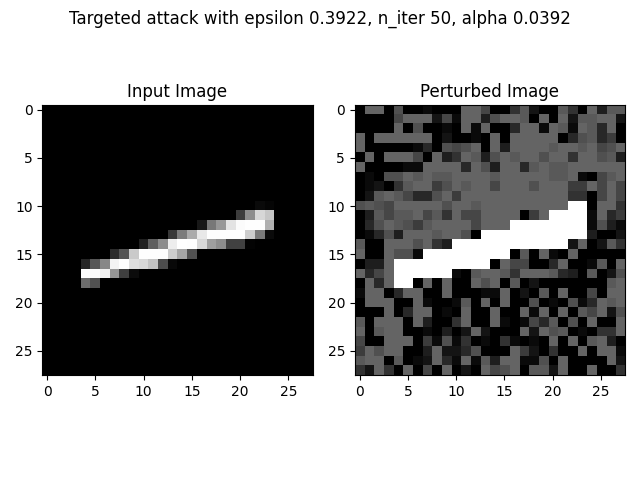
\includegraphics[trim={0 1.5cm 0cm 0}, width=.4\textwidth]{/Users/vashisth/Documents/GitHub/Intro_DL/IDL_HW3/HW3_tex/plots/Del6/Targeted/Targeted_attack__modA_e-0.3922_a-0.0392Img-2_iter50.png}
%     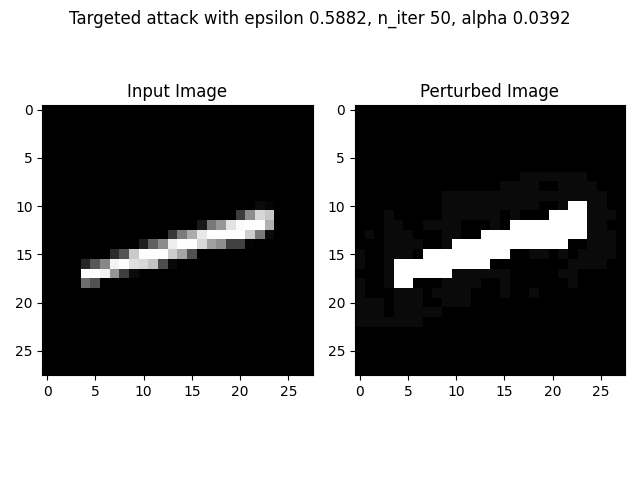
\includegraphics[trim = {0 1.5cm 0 0}, width = .4\textwidth] {/Users/vashisth/Documents/GitHub/Intro_DL/IDL_HW3/HW3_tex/plots/Del6/Targeted/Targeted_attack__modB_e-0.5882_a-0.0392Img-2_iter50.png}
%     %%%%%
%     \caption{Targeted Attack on Model B for Image with index 2 for different $\epsilon$ and $\alpha$ = 0.0392}
% \end{figure}


% \begin{figure}[H]
% \centering
% \includegraphics[width = .6 \textwidth]{/Users/vashisth/Documents/GitHub/Intro_DL/IDL_HW3/HW3_tex/plots/Del6/success_rate_plot_(PGD Targeted)_modA_iter50_a-0.0392.png}
% \caption{Success Rate and Accuracy Plot for Targeted Attack on Model A}
% \includegraphics[width = .6 \textwidth]{/Users/vashisth/Documents/GitHub/Intro_DL/IDL_HW3/HW3_tex/plots/Del6/success_rate_plot_(PGD Targeted)_modB_iter50_a-0.0392.png}
% \caption{Success Rate and Accuracy Plot for Targeted Attack on Model B}
% \end{figure}

% \end{solve}

%%%%%%%%%%%%%%%%%%%%%%%%%%%%%%%%%%%%%%%%%%%%
\newpage

\subsection{Task 2 (Targeted) vs Task 3 (Improved Targeted)}


\begin{solve}

The plots of purturbed images and the original images are shown below for both the tasks. The success rate and accuracy plots are also shown for both the models.

\textbf{Improved Targeted Attack}
For the improvement in the target attack, we follow the dicscussion from the recitation, where the TA said that LR decay, adptive techniques can be further used to improve the attack. However, we did not implement them.

In this version of improved attack, I implemeted the following updates to the PGD attack with Adam Momentum:
\begin{itemize}
    \item LR Decay was incorporated in the attack. The learning rate was decayed by a factor of 0.25 after every 10 iterations.
    \item Early Stopping was added in the attack. The attack was stopped if the loss was in the tolerance of $1e-3$ .
    \item Random Initialization was added to the attack. The attack was initialized with a random perturbation instead of always starting from the same perturbation.
    \item Lastly, an adaptive $\epsilon$ was used. The epsilon was increased by a factor of 1.2 after every 10 iterations.
\end{itemize}
% Note that in the case of targeted attacks, we used PGD. Given the value of $\alpha = .0392$, we see that the attack is quite visible even for $\epsilon \sim .04$


\textbf{Model A vs Model B for Targeted and Improved Targeted Attack}

\begin{itemize}
    \item For Targeted attacks, the success rate is higher for Model A than Model B. Infact we are unable to get any successful attack on Model B even with very high $\epsilon$ values as compared to Model A for the same $\alpha$ values.
    \item 
    We also see that the test accuracy does not change for model B during the attack, showing that not only we are failing in targeted attacks but we are also not able to misclassify the images in untargeted sense.
    This shows that Model B is more robust to attacks than Model A in this setting.

    \item We see the same is true for improved targeted attacks. The success rate is higher for Model A than Model B. Even for very high $epsilon$ values.
\end{itemize}


I have added the plots for other $\epsilon$ n the submission, but here are the plots for $\epsilon = 0.0980$ for both the models for both the attacks.

\begin{figure}[H]
    \centering
    \includegraphics[trim={0 1.5cm 0cm 0}, width=.5\textwidth]{/Users/vashisth/Documents/GitHub/Intro_DL/IDL_HW3/HW3_tex/plots/Del6/Targeted/Targeted_attack__modA_e-0.0980_a-0.0392Img-2_iter50.png}
    \caption{Targeted Attack on Model A with $\epsilon = 0.0980$, $\alpha = 0.0392$, 50 iterations}
    \centering
    \includegraphics[trim={0 1.5cm 0cm 0}, width=.5\textwidth]{/Users/vashisth/Documents/GitHub/Intro_DL/IDL_HW3/HW3_tex/plots/Del6/Targeted_improved/Targeted_improved_attack__modA_e-0.0980_a-0.0392Img-2_iter50.png}
    \caption{Improved Targeted Attack on Model A with $\epsilon = 0.0980$, $\alpha = 0.0392$, 50 iterations}
\end{figure}
We see that the improved attack is a bit harder to detect.

\begin{figure}[H]
    \centering
    \includegraphics[trim={0 1.5cm 0cm 0}, width=.5\textwidth]{/Users/vashisth/Documents/GitHub/Intro_DL/IDL_HW3/HW3_tex/plots/Del6/Targeted/Targeted_attack__modB_e-0.0980_a-0.0392Img-2_iter50.png}
    \caption{Targeted Attack on Model A with $\epsilon = 0.0980$, $\alpha = 0.0392$, 50 iterations}
    \centering
    \includegraphics[trim={0 0cm 0cm 0}, width=.5\textwidth]{/Users/vashisth/Documents/GitHub/Intro_DL/IDL_HW3/HW3_tex/plots/Del6/Targeted_improved/modB-0.0980_a-0.0392Img-2_iter50.png}
    \caption{Improved Targeted Attack on Model B with $\epsilon = 0.0980$, $\alpha = 0.0392$, 50 iterations}
\end{figure}



\begin{figure}[H]
    \centering
    \includegraphics[width = .45 \textwidth]{/Users/vashisth/Documents/GitHub/Intro_DL/IDL_HW3/HW3_tex/plots/Del6/success_rate_plot_(PGD Targeted)_modA_iter50_a-0.0392.png}
    \includegraphics[width = .45 \textwidth]{/Users/vashisth/Documents/GitHub/Intro_DL/IDL_HW3/HW3_tex/plots/Del6/success_rate_plot_(PGD Improved Targeted)_modA_iter50_a-0.0392.png}
    \caption{Success Rate and Accuracy Plot for Targeted Attack vs Improved Targeted Attack on Model A}
%%%%%%%%%
    \includegraphics[width = .45 \textwidth]{/Users/vashisth/Documents/GitHub/Intro_DL/IDL_HW3/HW3_tex/plots/Del6/success_rate_plot_(PGD Targeted)_modB_iter50_a-0.0392.png}
    \includegraphics[width = .45 \textwidth]{/Users/vashisth/Documents/GitHub/Intro_DL/IDL_HW3/HW3_tex/plots/Del6/success_rate_plot_(PGD Improved Targeted)_modB_iter50_a-0.0392.png}
    \caption{Success Rate and Accuracy Plot for Targeted Attack vs Improved Targeted Attack on Model B}
    \end{figure}
    
Again we see that despite the improved attack Model B doesnt get attacked. The success rate is 0 for Model B. The success rate for Model A is lower (by aroud .2) which might be due to not having the right hyper-parameters for momentum 1 and 2, and other scaling/decay factors.

\end{solve}




%%%%%%% 
\subsection{Bonus Task}


\begin{solve}
    For this $\alpha =  50/255$ was fixed for both the attacks. The $\epsilon$ values were $8/255, 16/255$ for the plots below.

\begin{figure}[H]
    \centering
    \includegraphics[width = .6 \textwidth]{/Users/vashisth/Documents/GitHub/Intro_DL/IDL_HW3/HW3_tex/plots/Del6/success_rate_plot_PGD Improved Targeted_modA (Bonus)_iter99_a-0.1961.png}

    \centering
    \includegraphics[width = .6 \textwidth]{//Users/vashisth/Documents/GitHub/Intro_DL/IDL_HW3/HW3_tex/plots/Del6/success_rate_plot_PGD Improved Targeted_modB (Bonus)_iter99_a-0.1961.png}

    \caption{Success Rate and Accuracy Plot for Improved Targeted Attack on Model A and B}
    \end{figure}

    For A we get a value of around $.00355$ for both $\epsilons$, for attack B we get success rate of $.010$ for smallest epsilon. I only got this for one run and got zero other runs. 

    Again showing Model B is very robust to the specific targeeted attack we are making in this case.
\end{solve}

%%%%%%%%%%%%%%%%%%%%%%%%%%%%%%%%%%%%%%%%%%%%

\newpage
% \input{temp}
\end{document}